\section{Геометрия решения}
1. \begin{figure}[ht!]
\center{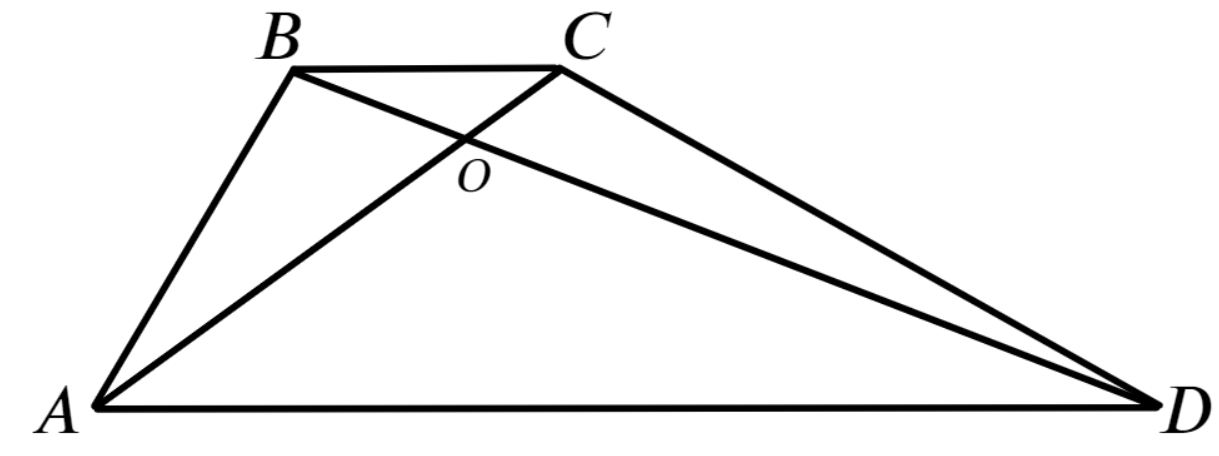
\includegraphics[scale=0.35]{g8-105.png}}
\end{figure}\\
Треугольники $AOD$ и $BOC$ подобны по двум углам ($\angle AOD$ и $\angle BOC$ вертикальные, $\angle BCO$ и $\angle OAD$ накрест лежащие). Раз
$\cfrac{S_{\Delta AOD}}{S_{\Delta BOC}}=16,$ коэффициент подобия равен $\sqrt{16}=4,$ поэтому $\cfrac{BC}{AD}=\cfrac{1}{4}.$\\
2. \begin{figure}[ht!]
\center{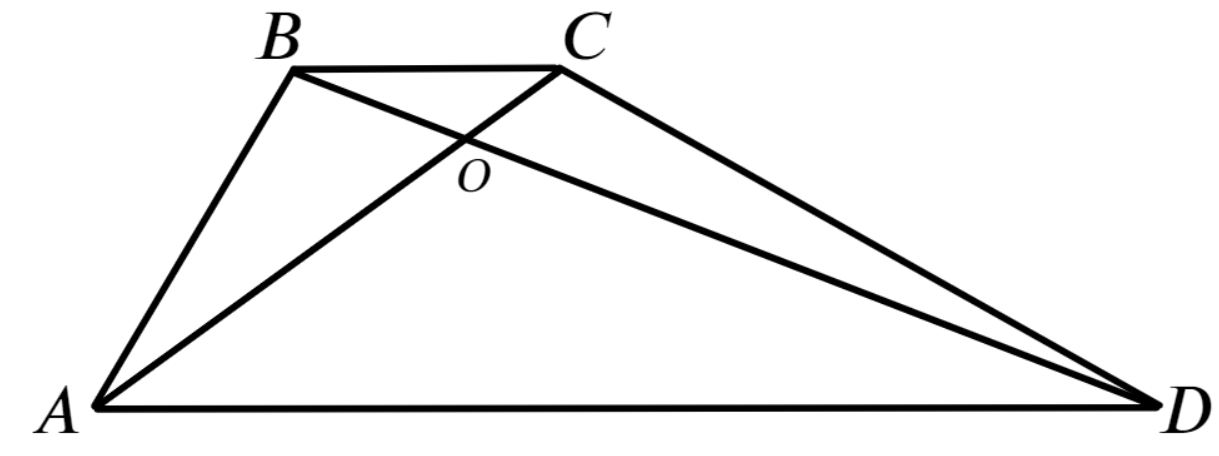
\includegraphics[scale=0.35]{g8-105.png}}
\end{figure}\\
Треугольники $BOC$ и $AOD$ подобны по двум углам ($\angle AOD$ и $\angle BOC$ вертикальные, $\angle BCO$ и $\angle OAD$ накрест лежащие). Раз
$\cfrac{S_{\Delta BOC}}{S_{\Delta AOD}}=\cfrac{1}{81},$ коэффициент подобия равен $\sqrt{\cfrac{1}{81}}=\cfrac{1}{9},$ поэтому $\cfrac{AD}{BC}=9.$\\
3. \begin{figure}[ht!]
\center{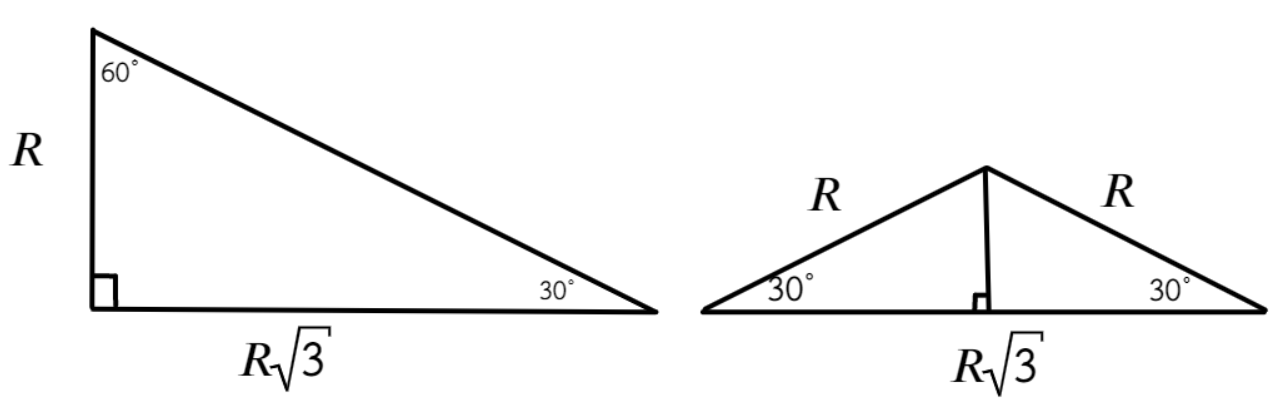
\includegraphics[scale=0.35]{g9-3.png}}
\end{figure}\\
Пусть напротив сторон с величинами $R$ и $R\sqrt{3}$ лежат углы $\alpha$ и $\beta.$ Тогда по теореме синусов $\cfrac{R}{\sin(\alpha)}=\cfrac{R\sqrt{3}}{\sin(\beta)}=2R\Rightarrow \alpha=30^\circ\text{ или }150^\circ,\ \beta=60^\circ\text{ или }120^\circ.$
Возможны два случая $\alpha=30^\circ,\ \beta=60^\circ$ или $\alpha=30^\circ,\ \beta=120^\circ.$ Если $\alpha=150^\circ,$ то сумма углов треугольника получается больше $180^\circ$ при любом возможном значении $\beta.$ В первом случае треугольник является прямоугольным и его площадь равна $S=\cfrac{R\cdot R\sqrt{3}}{2}=\cfrac{\sqrt{3}}{2}R^2.$ Во втором случае треугольник является равнобедренным ($180^\circ-120^\circ-30^\circ=30^\circ$), опустим высоту из его вершины, она равна $R\sin(30^\circ)=\cfrac{1}{2}R.$ Тогда площадь треугольника равна $S=\cfrac{1}{2}\cdot\cfrac{1}{2}R\cdot R\sqrt{3}=\cfrac{\sqrt{3}}{4}R^2.$
ewpage
oindent
4. \begin{figure}[ht!]
\center{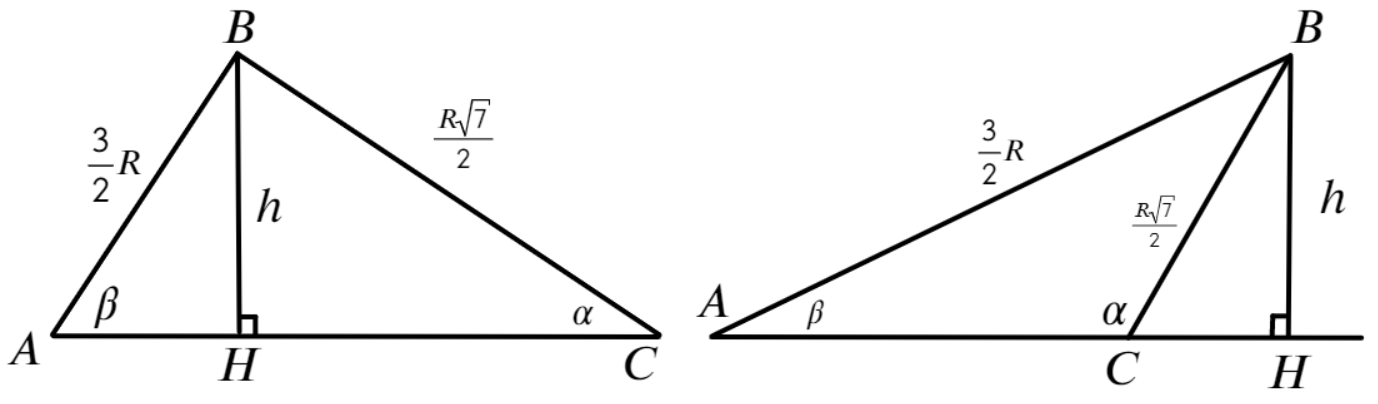
\includegraphics[scale=0.35]{g9-4.png}}
\end{figure}\\
По теореме синусов $\cfrac{\cfrac{3}{2}R}{\sin(\alpha)}=\cfrac{R\cfrac{\sqrt{7}}{2}}{\sin(\beta)}=2R,$ значит $\sin(\alpha)=\cfrac{3}{4},\ \sin(\beta)=\cfrac{\sqrt{7}}{4}.$ Так как $\cfrac{3}{2}>\cfrac{\sqrt{7}}{2},\ \alpha>\beta,$ поэтому тупым может быть только угол $\alpha$ (если угол $\beta$ является тупым, то сумма углов треугольника больше $180^\circ.$)Опустим высоту из точки $B,$ тогда $h=\cfrac{3}{2}R \sin(\beta)=\cfrac{3\sqrt{7}}{8}R.$ Возможны два случае: точка $H$ лежит на стороне $AC$ или вне её. В первом случае $AC=AH+HC=\cfrac{3}{2}R \cos(\beta)+R\cfrac{\sqrt{7}}{2}\cos(\alpha)=
\cfrac{3}{2}R \sqrt{1-\cfrac{7}{16}}+R\cfrac{\sqrt{7}}{2}\sqrt{1-\cfrac{9}{16}}=2R.$ Тогда $S=\cfrac{1}{2}\cdot\cfrac{3\sqrt{7}}{8}R\cdot
2R=\cfrac{3\sqrt{7}}{8}R^2.$ Во втором случае $AC=AH-CH=\cfrac{3}{2}R \cos(\beta)-R\cfrac{\sqrt{7}}{2}\cos(180^\circ-\alpha)=
\cfrac{3}{2}R \sqrt{1-\cfrac{7}{16}}-R\cfrac{\sqrt{7}}{2}\sqrt{1-\cfrac{9}{16}}=\cfrac{R}{4}.$ Тогда $S=\cfrac{1}{2}\cdot\cfrac{3\sqrt{7}}{8}R\cdot\cfrac{R}{4}=\cfrac{3\sqrt{7}}{64}R^2.$\\
5. \begin{figure}[ht!]
\center{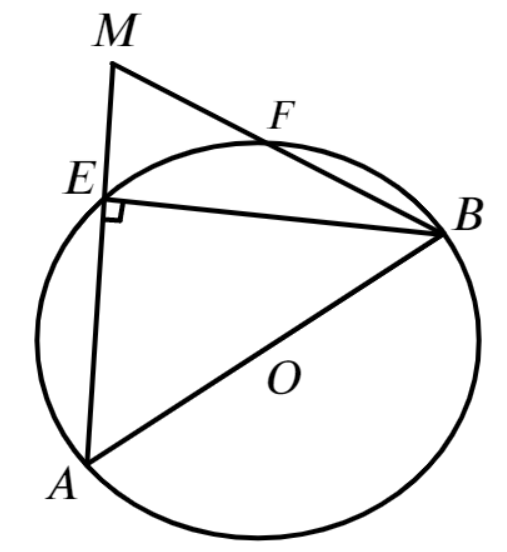
\includegraphics[scale=0.35]{g9-5.png}}
\end{figure}\\
Угол $AEB$ опирается на диаметр $AB,$ а значит равен $90^\circ.$ Тогда $EB=\sqrt{AB^2-AE^2}=\sqrt{25-9}=4.$ Тогда $S_{\Delta AMB}=\cfrac{1}{2}\cdot4\cdot (3+2)=10.$\\
6. \begin{figure}[ht!]
\center{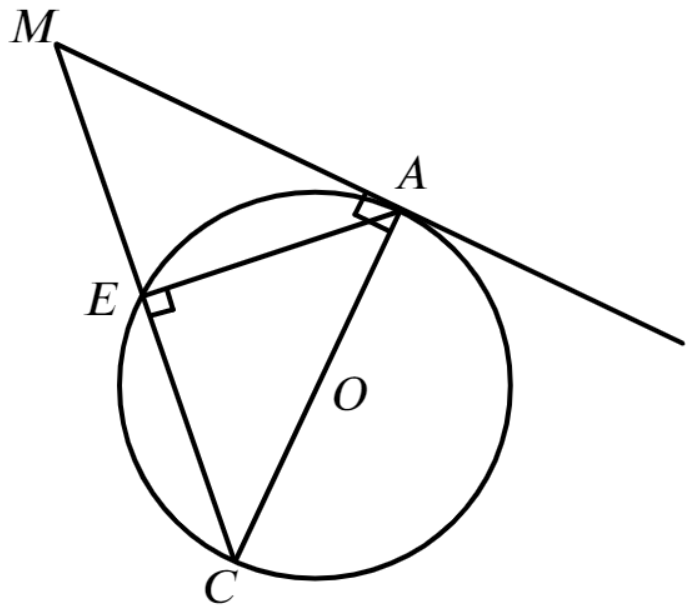
\includegraphics[scale=0.35]{g9-6.png}}
\end{figure}\\
Угол $AEC$ опирается на диаметр $AC,$ а $\angle MAC$ --- угол между радиусом и касательной, значит они равны $90^\circ.$ Тогда $MAC$ является прямоугольным треугольником, а $AE$ --- его высота. Найдём $MC=\sqrt{MA^2+AC^2}=\sqrt{25+144}=13$ и посчитаем его площадь двумя способами: $S=\cfrac{5\cdot12}{2}=\cfrac{AE\cdot13}{2},$ значит $AE=\cfrac{60}{13}.$\\
7. Преобразуем соотношение: $p(p-a)=\cfrac{3}{4}bc,\ \cfrac{a+b+c}{2}\cdot\cfrac{b+c-a}{2}=\cfrac{3}{4}bc,\ b^2+2bc+c^2-a^2=3bc,\ a^2=b^2+c^2-bc.$ С другой стороны, по теореме косинусов имеем $a^2=b^2+c^2-2bc\cos(\angle A),$ откуда $\cos(\angle A)=\cfrac{1}{2},\ \angle A=60^\circ.$\\
8. По теореме косинусов имеем $a^2=b^2+c^2-2bc\cos(\angle A),$ откуда $S=\cfrac{1}{4}(b^2+c^2-a^2)=\cfrac{1}{4}\cdot 2bc\cos(\angle A)=\cfrac{1}{2}bc\cos(\angle A).$ С другой стороны, $S=\cfrac{1}{2}bc\sin(\angle A),$ поэтому $\sin(\angle A)=\cos(\angle A),$ значит $tg(\angle A)=1,\ \angle A=45^\circ.$\\
9. \begin{figure}[ht!]
\center{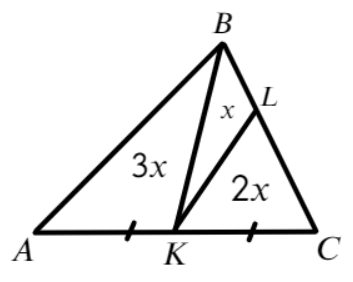
\includegraphics[scale=0.35]{g9-9.png}}
\end{figure}\\
Если треугольники имеют общую высоту, их площади относятся так же, как основания, к которым проведена эта высота. Поэтому $S_{\Delta BLK}=x,\ S_{\Delta KLC}=2x,$ а $S_{\Delta ABK}=S_{\Delta BKC}=x+2x=3x.$ Поэтому $\cfrac{S_{\Delta KLC}}{S_{ABLK}}=\cfrac{2x}{3x+x}=\cfrac{1}{2}.$\\
10. \begin{figure}[ht!]
\center{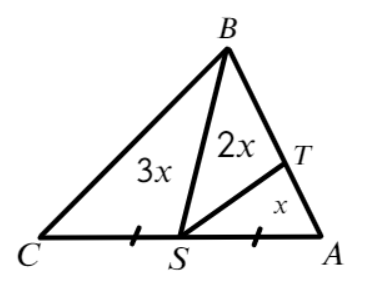
\includegraphics[scale=0.35]{g9-10.png}}
\end{figure}\\
Если треугольники имеют общую высоту, их площади относятся так же, как основания, к которым проведена эта высота. Поэтому $S_{\Delta ATS}=x,\ S_{\Delta BTS}=2x,$ а $S_{\Delta BCS}=S_{\Delta BAS}=x+2x=3x.$ Поэтому $\cfrac{S_{\Delta ATS}}{S_{CBTS}}=\cfrac{x}{3x+2x}=\cfrac{1}{5}.$\\
11. \begin{figure}[ht!]
\center{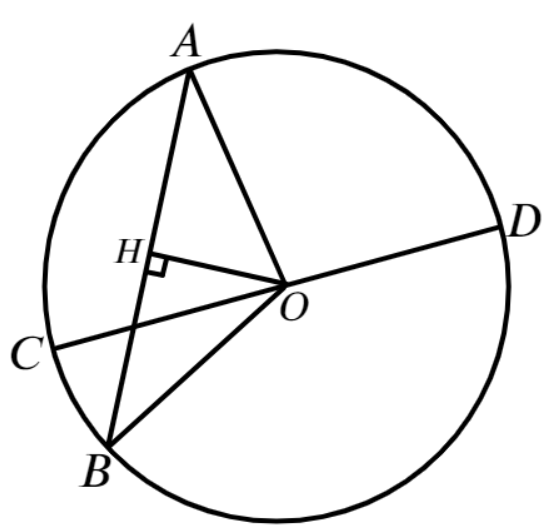
\includegraphics[scale=0.35]{g9-11.png}}
\end{figure}\\
В треугольнике $OAB$ стороны $OA$ и $OB$ равны, так как являются радиусами. Тогда он равнобедренный и $OH$ является не только высотой, но и медианой, а поэтому $OC=OB=\sqrt{OH^2+HB^2}=\sqrt{64+16}=4\sqrt{5}.$
ewpage
oindent
12. \begin{figure}[ht!]
\center{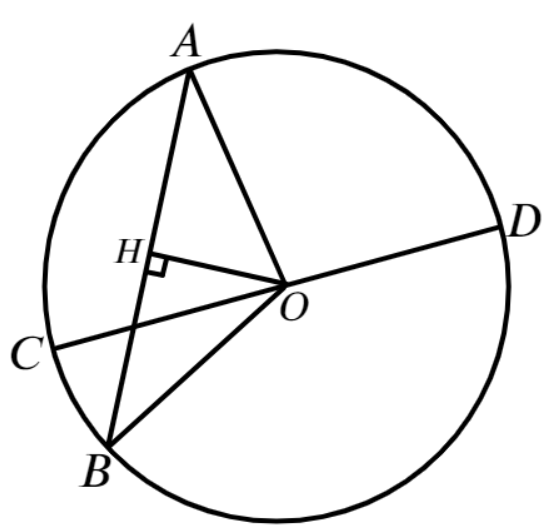
\includegraphics[scale=0.35]{g9-11.png}}
\end{figure}\\
В треугольнике $OAB$ стороны $OA$ и $OB$ равны, так как являются радиусами. Тогда он равнобедренный и $OH$ является не только высотой, но и медианой, а поэтому $AB=2BH=2\sqrt{100-16}=4\sqrt{21}.$\\
13. \begin{figure}[ht!]
\center{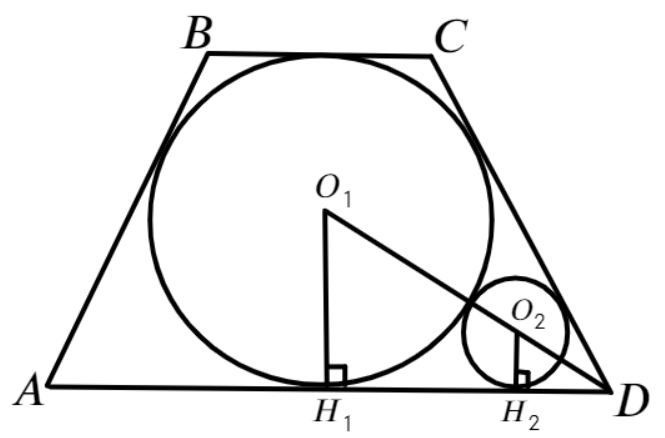
\includegraphics[scale=0.35]{g9-13.png}}
\end{figure}\\
Так как трапеция является описанной, $AB+CD=BC+AD,\ 2AB=2+8=10,\ AB=5.$ Опустив две высоты из вершин $B$ и $C,$ можно найти высоту трапеции: $h=\sqrt{5^2-\left(\cfrac{8-2}{2}
ight)^2}=4.$ Тогда радиус большей окружности равен $4:2=2.$ Раз обе окружности касаются сторон $AD$ и $CD,$ их центры лежат на биссектрисе угла $D.$ Проведём перпендикуляры $O_1H_1$ и $O_2H_2$ к точкам касания. Найдём $O_1D=\sqrt{4^2+2^2}=2\sqrt{5}.$ Пусть радиус меньшей окружности равен $x,$ тогда  $O_2D=2\sqrt{5}-2-x.$ Из подобия треугольников $O_1H_1D$ и $O_2H_2D$ (по двум углам) получаем соотношение $\cfrac{2\sqrt{5}-2-x }{2\sqrt{5}}=\cfrac{x}{2},$ откуда $4\sqrt{5}-4-2x=2\sqrt{5}x,\ 2x(1+\sqrt{5})=4(\sqrt{5}-1),\ x=\cfrac{2(\sqrt{5}-1)}{1+\sqrt{5}}=3-\sqrt{5}.$\\
14. \begin{figure}[ht!]
\center{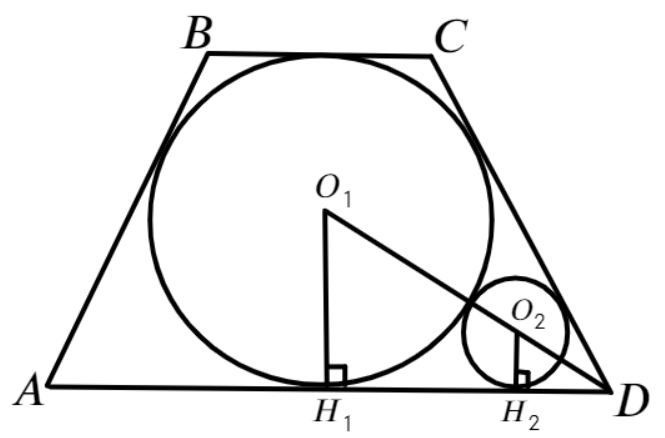
\includegraphics[scale=0.35]{g9-13.png}}
\end{figure}\\
Высота трапеции в два раза больше радиуса вписанной окружности и равна $2\cdot4=8.$ Пусть меньшее основания равны $a$ и $b,\ a>b,$ тогда опустив две высоты из точек $B$ и $C,$ найдём $\cfrac{a-b}{2}=\sqrt{100-64}=6,\ a-b=12.$ Так как трапеция является описанной, $a+b=10+10=20,$ откуда $2a=12+20=32,\ a=16,\ b=16-12=4.$ Раз обе окружности касаются сторон $AD$ и $CD,$ их центры лежат на биссектрисе угла $D.$ Проведём перпендикуляры $O_1H_1$ и $O_2H_2$ к точкам касания. Найдём $O_1D=\sqrt{8^2+4^2}=4\sqrt{5}.$ Пусть радиус меньшей окружности равен $x,$ тогда  $O_2D=4\sqrt{5}-4-x.$ Из подобия треугольников $O_1H_1D$ и $O_2H_2D$ (по двум углам) получаем соотношение $\cfrac{4\sqrt{5}-4-x }{4\sqrt{5}}=\cfrac{x}{4},$ откуда $16\sqrt{5}-16-4x=4\sqrt{5}x,\ 4x(1+\sqrt{5})=16(\sqrt{5}-1),\ x=\cfrac{4(\sqrt{5}-1)}{1+\sqrt{5}}=6-2\sqrt{5}.$\\
15. \begin{figure}[ht!]
\center{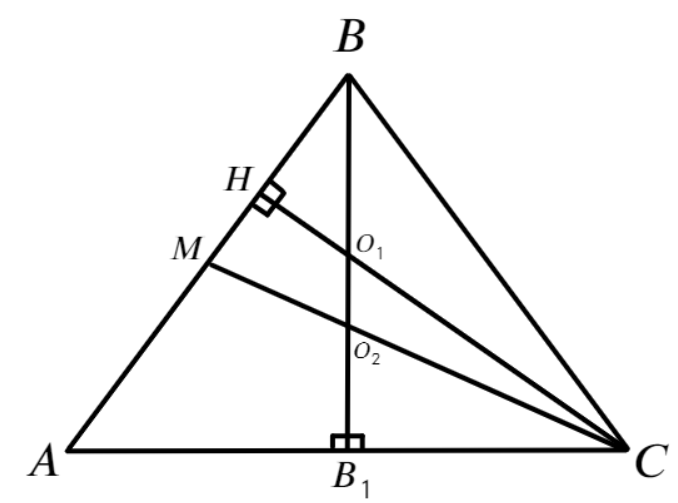
\includegraphics[scale=0.35]{g9-15.png}}
\end{figure}\\
Пусть $CH$ высота, $CM$ медиана, а $BB_1$ --- и то, и другое. По теореме Пифагора $BB_1=\sqrt{5^2-3^2}=4.$ Так как медианы делятся точкой их пересечения в отношении $2:1,$ имеем $O_2B_1=\cfrac{1}{3}\cdot4=\cfrac{4}{3}.$ В четырёхугольнике $B_1HBC$ равны углы $BHC$ и $BB_1C,$ образованные противоположными сторонами и разными диагоналями, значит он является вписанным и поэтому $\angle B_1CO_1=\angle B_1BH.$ Тогда треугольники $CO_1B_1$ и $B_1BA$ подобны по двум углам и  $\cfrac{CB_1}{BB_1}=\cfrac{B_1O_1}{AB_1},\ \cfrac{3}{4}=\cfrac{B_1O_1}{3}\Rightarrow B_1O_1=\cfrac{9}{4}.$ Таким образом, $O_1O_2=B_1O_1-O_2B_1=\cfrac{9}{4}-\cfrac{4}{3}=\cfrac{11}{12}.$\\
16. \begin{figure}[ht!]
\center{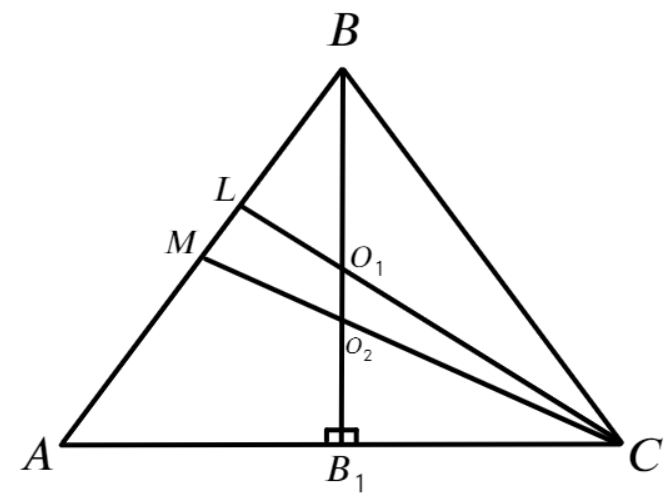
\includegraphics[scale=0.35]{g9-16.png}}
\end{figure}\\
Пусть $CL$ биссектриса, $CM$ медиана, а $BB_1$ --- и то, и другое. По теореме Пифагора $BB_1=\sqrt{5^2-3^2}=4.$ Так как медианы делятся точкой их пересечения в отношении $2:1,$ имеем $O_2B_1=\cfrac{1}{3}\cdot4=\cfrac{4}{3}.$ По свойству основания биссектрисы имеем $\cfrac{BO_1}{B_1O_1}=\cfrac{BC}{CB_1}=\cfrac{5}{3},$ откуда $O_1B_1=\cfrac{3}{8}\cdot4=\cfrac{3}{2}.$ Таким образом, $O_1O_2=B_1O_1-O_2B_1=\cfrac{3}{2}-\cfrac{4}{3}=\cfrac{1}{6}.$\\
17. \begin{figure}[ht!]
\center{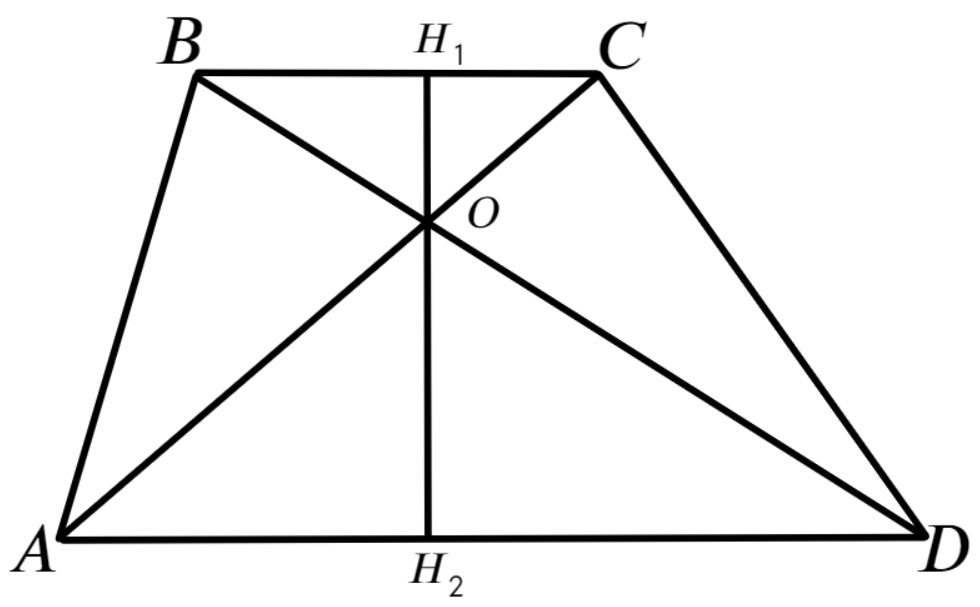
\includegraphics[scale=0.35]{g9-17.png}}
\end{figure}\\
Треугольники $BOC$ и $AOD$ подобны по двум углам (накрест лежащим $OBC$ с $ADO$ и $OAD$ с $OCB$), коэффициент подобия $k=\sqrt{\cfrac{S_{\Delta BOC}}{S_{\Delta AOD}}}=\sqrt{\cfrac{a^2}{b^2}}=\cfrac{a}{b}.$ Пусть тогда $BC=ax,\ AD=bx.$ Высоты в подобных треугольника относятся друг к другу с тем же коэффициентом подобия, поэтому можно считать, что $OH_1=ay,\ OH_2=by.$ При этом $S_{\Delta BOC}=\cfrac{1}{2}\cdot ay\cdot ax=a^2,$ откуда $xy=2.$ Таким образом, $S_{ABCD}=\cfrac{BC+AD}{2}\cdot H_1H_2=\cfrac{ax+bx}{2}\cdot(ay+by)=(a+b)^2.$\\
18. \begin{figure}[ht!]
\center{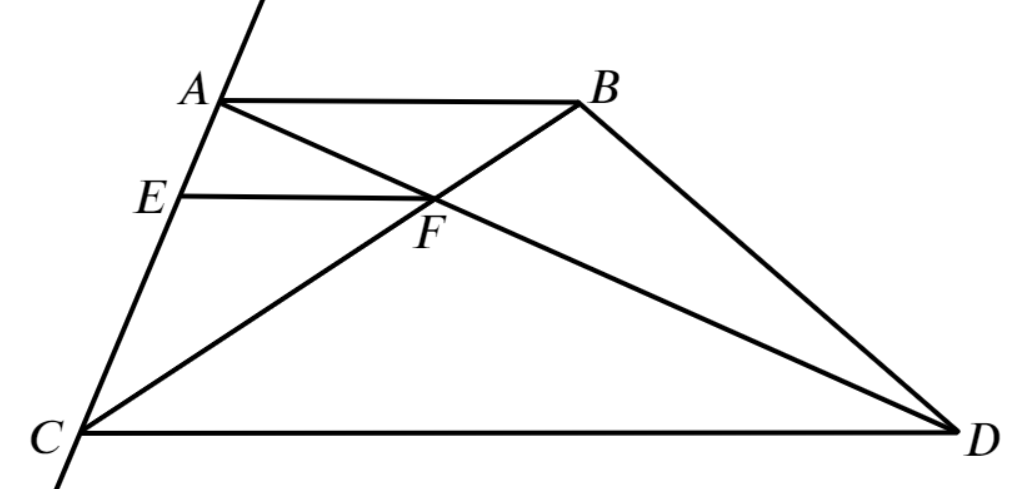
\includegraphics[scale=0.35]{g9-18.png}}
\end{figure}\\
Треугольники $ABF$ и $DCF$ подобны по двум углам ($\angle FAB=\angle FDC$ и $\angle FBA=\angle FCD$ как накрест лежащие), значит $\cfrac{BF}{CF}=\cfrac{AB}{CD}.$ Треугольники $CEF$ и $CAB$ также подобны по двум углам ($\angle CEF=\angle CAB$ и $\angle CFE=\angle CBA$ как соответственные), значит $\cfrac{CB}{CF}=\cfrac{AB}{EF}\Rightarrow \cfrac{CF+BF}{CF}=\cfrac{AB}{EF}\Rightarrow 1+\cfrac{AB}{CD}=\cfrac{AB}{EF}
\Rightarrow \cfrac{1}{AB}+\cfrac{1}{CD}=\cfrac{1}{EF},$ ч.т.д.\\
19. \begin{figure}[ht!]
\center{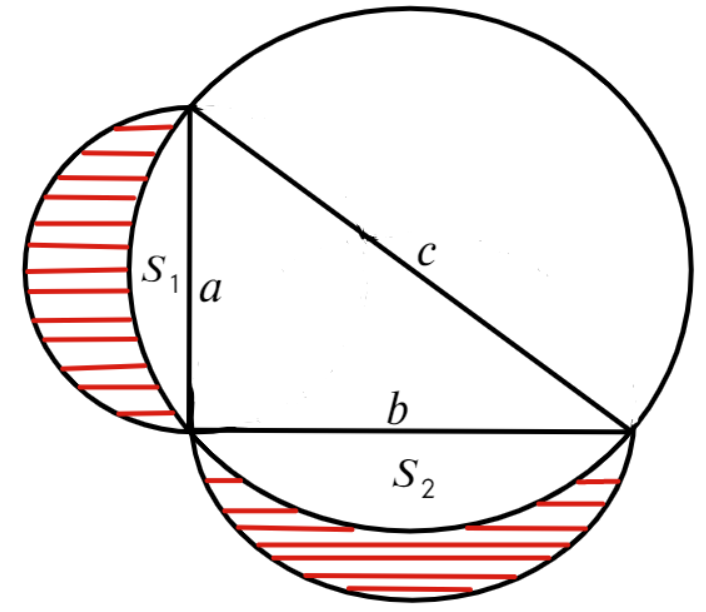
\includegraphics[scale=0.35]{g9-19.png}}
\end{figure}\\
Пусть катеты треугольника равны $a$ и $b,$ а гипотенуза --- $c.$ Искомая сумма площадей равна $\cfrac{\pi a^2}{8}-S_1+\cfrac{\pi b^2}{8}-S_2,$ где $S_1$ и $S_2$ --- площади сегментов, отсекаемых катетами треугольника от описанного круга. Выразим $S_1+S_2=\cfrac{\pi c^2}{8}-\cfrac{ab}{2},$ тогда
$\cfrac{\pi a^2}{8}+\cfrac{\pi b^2}{8}-(S_1+S_2)=\cfrac{\pi a^2}{8}+\cfrac{\pi b^2}{8}-\cfrac{\pi c^2}{8}+\cfrac{ab}{2}=\cfrac{a^2+b^2-c^2}{8}+\cfrac{ab}{2}=
\cfrac{ab}{2}=1.$
ewpage
oindent
20. \begin{figure}[ht!]
\center{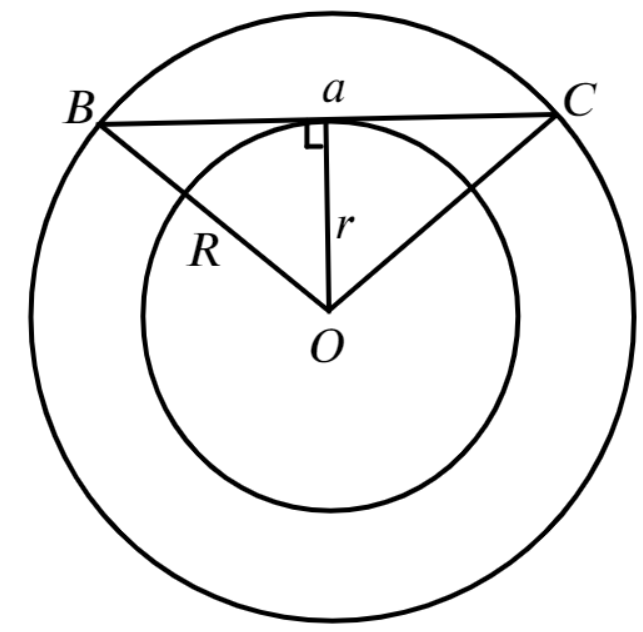
\includegraphics[scale=0.35]{g9-20.png}}
\end{figure}\\
Пусть длина хорды равна $a,$ тогда площадь построенного на ней круга равна $\cfrac{\pi a^2}{4}.$ Если радиусы окружностей равны $R$ и $r,$ то площадь кольца между ними равна $\pi(R^2-r^2).$ Треугольник $OBC$ является равнобедренным ($OB=OC),$ значит в нём высота совпадает с медианой и по теореме Пифагора $R^2-r^2=\cfrac{a^2}{4},$ откуда $\pi(R^2-r^2)=\cfrac{\pi a^2}{4},$ ч.т.д.\\
21. \begin{figure}[ht!]
\center{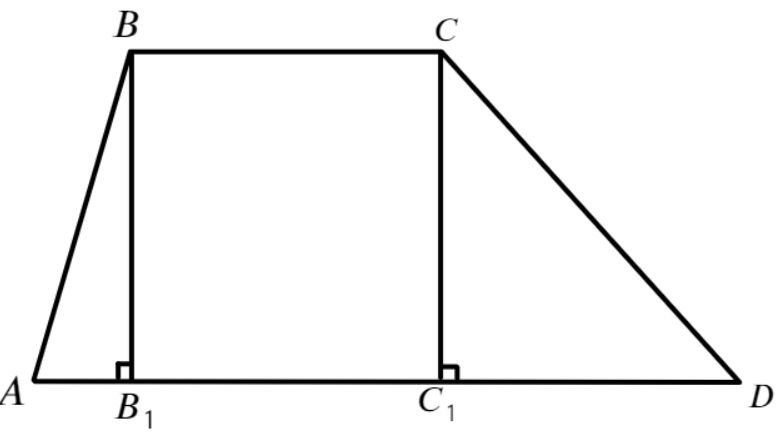
\includegraphics[scale=0.35]{g9-21.png}}
\end{figure}\\
Опустим высоты $BB_1$ и $CC_1.$ Пусть $AB=17$см, $BC=16$см, $CD=25$см, $AD=44$см, $AB_1=x.$ Тогда $C_1D=44-16-x=28-x$ и по теореме Пифагора имеем равенства
$17^2-x^2=BB_1^2=CC_1^2=25^2-(28-x)^2,\ 289-x^2=625-784+56x-x^2,\ 56x=448,\ x=8$см. Таким образом, $BB_1=\sqrt{289-64}=15$см и $S_{ABCD}=15\cdot\cfrac{16+44}{2}=450\text{ см}^2.$\\
22. \begin{figure}[ht!]
\center{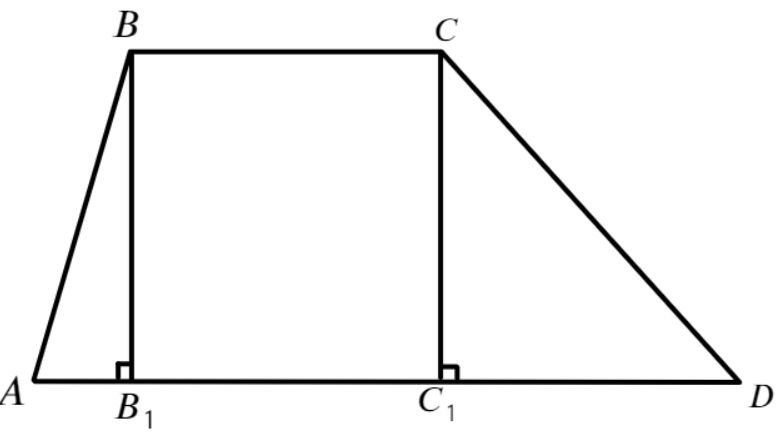
\includegraphics[scale=0.35]{g9-21.png}}
\end{figure}\\
Опустим высоты $BB_1$ и $CC_1.$ Пусть $AB=5$см, $BC=6$см, $CD=12$см, $AD=7$см, $AB_1=x.$ Тогда $C_1D=7-6-x=1-x$ и по теореме Пифагора имеем равенства
$5^2-x^2=BB_1^2=CC_1^2=12^2-(1-x)^2,\ 25-x^2=144-1+2x-x^2,\ 2x=-118,\ x=-59$. Полученный отрицательный результат говорит о том, что на самом деле картинка выглядит по-другому и высота из точки $B$ падает на продолжение основания $AD.$
ewpage
oindent
\begin{figure}[ht!]
\center{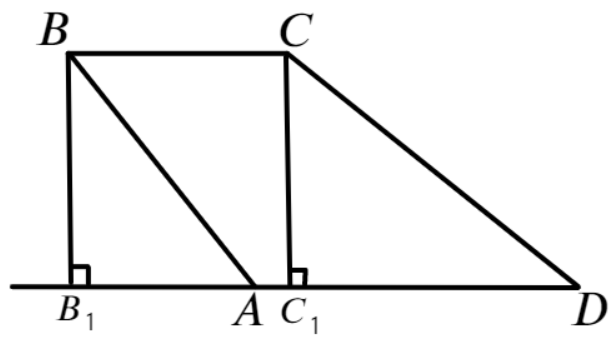
\includegraphics[scale=0.35]{g9-21-1.png}}
\end{figure}\\
Тогда если $AB_1=x,$ то $AC_1=6-x,\ C_1D=7-(6-x)=x+1$ и $5^2-x^2=BB_1^2=CC_1^2=12^2-(x+1)^2,\ 25-x^2=144-1-2x-x^2,\ 2x=118,\ x=59$см. Но тогда в треугольнике
$ABB_1$ катет длиннее гипотенузы, что невозможно, значит такой трапеции не существует.\\
23. \begin{figure}[ht!]
\center{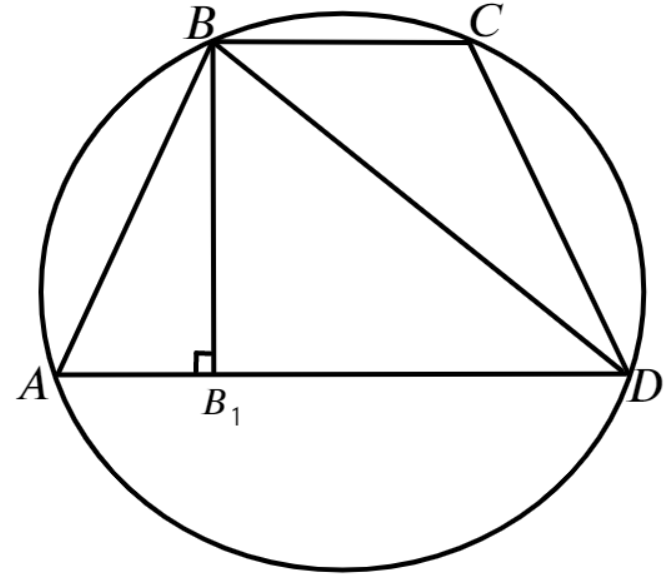
\includegraphics[scale=0.35]{g9-22.png}}
\end{figure}\\
Если трапеция является вписанной, то она равнобедренная. Если трапеция является описанной, то суммы её противоположных сторон равны, значит боковая сторона трапеции равна $\cfrac{4+16}{2}=10$см. Опустим высоту $BB_1,$ тогда $AB_1=\cfrac{16-4}{2}=6$см и $BB_1=\sqrt{100-36}=8$см. Высота трапеции равна диаметру вписанной окружности, значит её радиус равен $8:2=4$см. Описанная окружность этой трапеции является также и описанной окружностью треугольника $ABD.$ Найдём $B_1D=16-6=10$см, $BD=\sqrt{100+64}=2\sqrt{41}$см. Из треугольника $ABB_1$ имеем $\sin(\angle A)=\cfrac{8}{10}=\cfrac{4}{5},$ тогда по теореме синусов для треугольника $ABD$ получим $2R=\cfrac{2\sqrt{41}}{\cfrac{4}{5}}=\cfrac{5\sqrt{41}}{2},\ R=\cfrac{5\sqrt{41}}{4}$см.\\
24. \begin{figure}[ht!]
\center{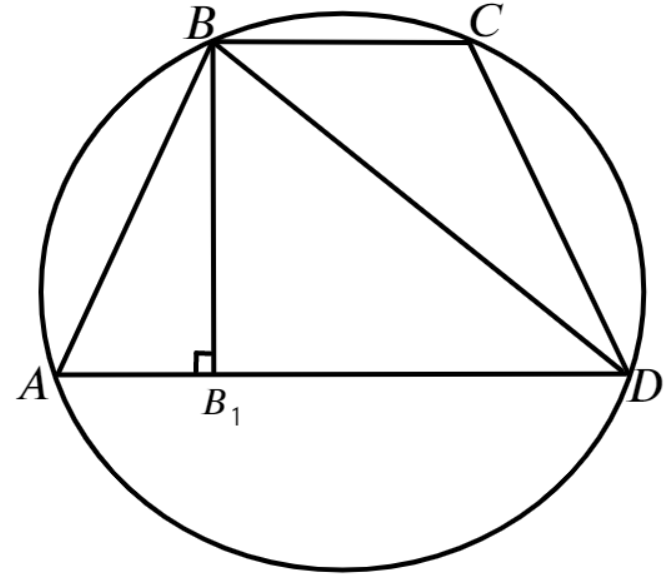
\includegraphics[scale=0.35]{g9-22.png}}
\end{figure}\\
Если трапеция является вписанной, то она равнобедренная. Если трапеция является описанной, то суммы её противоположных сторон равны, значит боковая сторона трапеции равна $\cfrac{2+14}{2}=8$см. Опустим высоту $BB_1,$ тогда $BB_1=2\cdot4=8$см, так как высота трапеции равна диаметру вписанной окружности. В таком случае высота трапеции оказалась равна её боковой стороне, что невозможно (в этом случае трапеция становится прямоугольником). Значит, трапеции с заданными параметрами не существует.\\
25. Найдём $\angle B=180^\circ-75^\circ-60^\circ=45^\circ.$ Запишем теорему синусов: $\cfrac{AC}{\sin(\angle B)}=\cfrac{AB}{\sin(\angle C)},$\\$
\cfrac{\sqrt{2}}{\cfrac{\sqrt{2}}{2}}=\cfrac{AB}{\cfrac{\sqrt{3}}{2}},\ AB=\sqrt{3}.$\\
26. Найдём $\angle C=180^\circ-75^\circ-45^\circ=60^\circ.$ Запишем теорему синусов: $\cfrac{AC}{\sin(\angle B)}=\cfrac{AB}{\sin(\angle C)},$\\$
\cfrac{AC}{\cfrac{\sqrt{2}}{2}}=\cfrac{\sqrt{3}}{\cfrac{\sqrt{3}}{2}},\ AB=\sqrt{2}.$\\
27. Вектора перпендикулярны тогда и только тогда, когда их скалярное произведение равно нулю, значит $\vec{a}\cdot\vec{b}=4x-30=0,\ x=7,5.$\\
28. Вектора перпендикулярны тогда и только тогда, когда их скалярное произведение равно нулю, значит $\vec{a}\cdot\vec{b}=5x-12=0,\ x=2,4.$\\
29. \begin{figure}[ht!]
\center{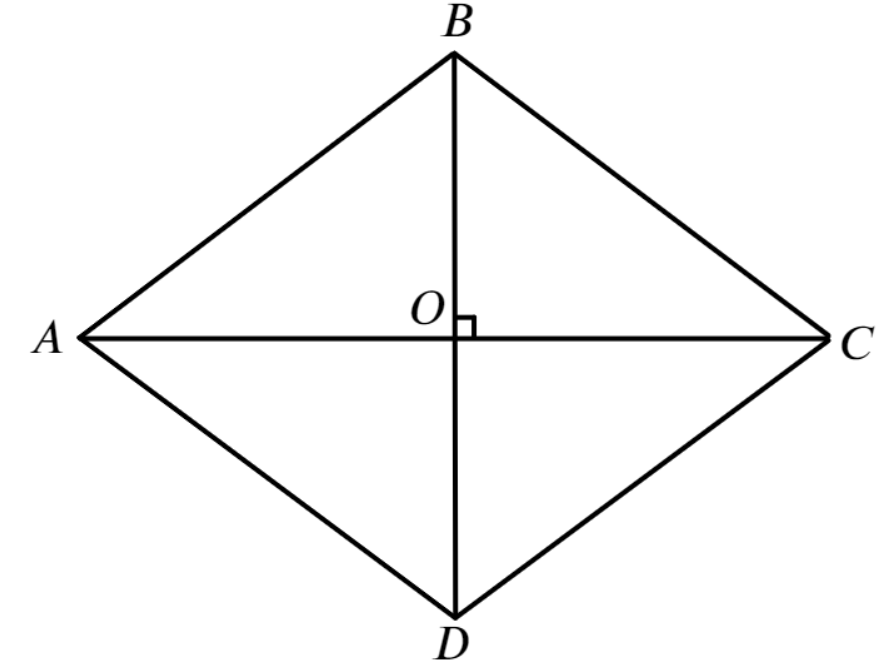
\includegraphics[scale=0.35]{g9-29.png}}
\end{figure}\\
В ромбе диагонали перпендикулярны и делятся точкой пересечения пополам. Если $BD=12$см, то по теореме Пифагора $AO=\sqrt{100-36}=8$см, значит вторая диагональ равна 16 см. Площадь ромба равна половине произведения диагоналей, значит $S=\cfrac{1}{2}\cdot12\cdot16=96\text{ см}^2.$\\
30. \begin{figure}[ht!]
\center{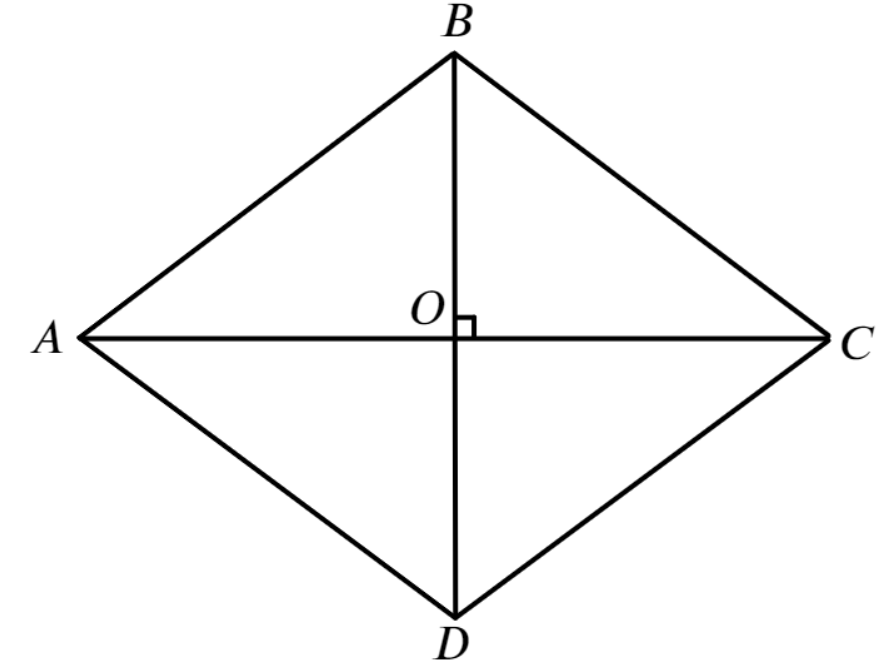
\includegraphics[scale=0.35]{g9-29.png}}
\end{figure}\\
В ромбе диагонали перпендикулярны и делятся точкой пересечения пополам. Если $BD=6$см, то по теореме Пифагора $AO=\sqrt{25-9}=4$см, значит вторая диагональ равна 8 см. Площадь ромба равна половине произведения диагоналей, значит $S=\cfrac{1}{2}\cdot6\cdot8=24\text{ см}^2.$
ewpage
oindent
31. \begin{figure}[ht!]
\center{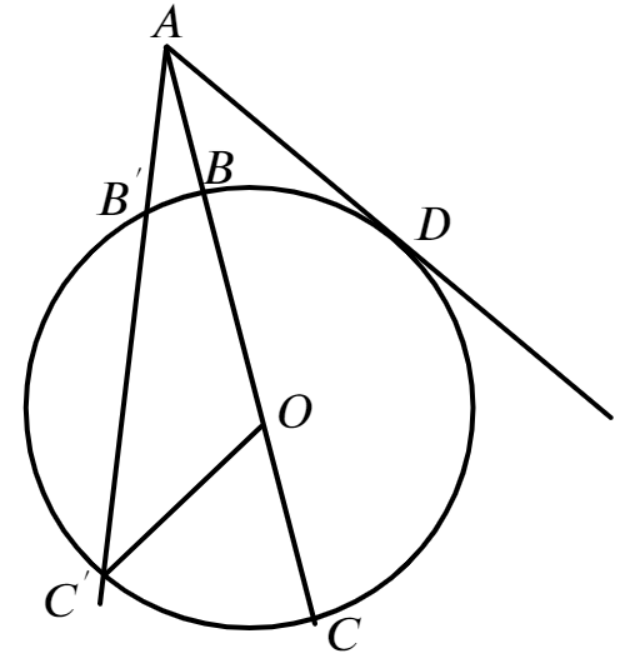
\includegraphics[scale=0.35]{g9-31.png}}
\end{figure}\\
Сначала покажем, что наибольшая секущая проходит через центр окружности. Проведём проходящую через центр секущую $AC$ и какую-то другую секущую $AC'.$ Тогда по неравенству треугольника для треугольника $AOC'$ имеем $AC'<AO+OC'=AO+OC=AC,$ ч.т.д. Пусть радиус окружности равен $R,$ а $AB=x.$ По свойству касательной и секущей
запишем равенство $AD^2=AB\cdot AC,\ 400=x\cdot 50,\ x=8$см, при этом $x+2R=50,\ R=21$см.\\
32. \begin{figure}[ht!]
\center{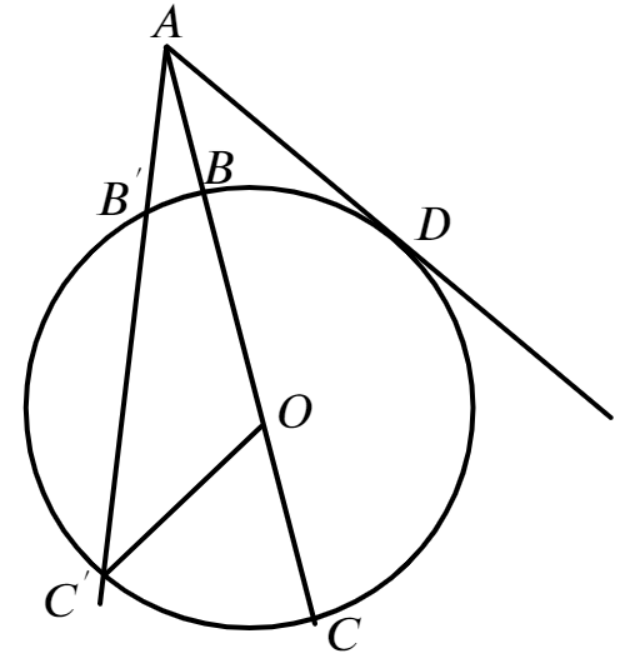
\includegraphics[scale=0.35]{g9-31.png}}
\end{figure}\\
Сначала покажем, что наибольшая секущая проходит через центр окружности. Проведём проходящую через центр секущую $AC$ и какую-то другую секущую $AC'.$ Тогда по неравенству треугольника для треугольника $AOC'$ имеем $AC'<AO+OC'=AO+OC=AC,$ ч.т.д. Пусть радиус окружности равен $R,$ а $AB=x.$ По свойству касательной и секущей
запишем равенство $AD^2=AB\cdot AC,\ 144=x\cdot 36,\ x=4$см, при этом $x+2R=36,\ R=16$см.\\
33. $|\vec{a}|=\sqrt{1+t^2}=|\vec{b}|=\sqrt{(t+2)^2+(-t)^2},$ значит $1+t^2=t^2+4t+4+t^2,\ t^2+4t+3=0,\ t=-3$ или $t=-1.$\\
34. $|\vec{a}|=\sqrt{1+(-t)^2}=|\vec{b}|=\sqrt{(2-t)^2+t^2},$ значит $1+t^2=t^2-4t+4+t^2,\ t^2-4t+3=0,\ t=3$ или $t=1.$\\
35. Пусть основание равно $4x,$ а боковая сторона --- $3x.$ Найдём площадь треугольника разными способами. Выразим $p=\cfrac{3x+3x+4x}{2}=5x,$ тогда по формуле Герона она равна \\$S=\sqrt{5x\cdot2x\cdot 2x\cdot x}=2\sqrt{5}x^2.$ С другой стороны, $S=rp=5xr.$ Тогда $5xr=2\sqrt{5}x^2,\ r=\cfrac{2\sqrt{5}}{5}x.$ Также площадь можно найти как половину произведения высоты на сторону и возможно два случая: высота проведена к основанию или к боковой стороне. В первом случае $\cfrac{1}{2}\cdot20\cdot4x=2\sqrt{5}x^2,\ x=\cfrac{20}{\sqrt{5}},$ тогда $r=\cfrac{2\sqrt{5}}{5}\cdot\cfrac{20}{\sqrt{5}}=8.$ Во втором случае
$\cfrac{1}{2}\cdot20\cdot3x=2\sqrt{5}x^2,\ x=\cfrac{15}{\sqrt{5}},$ тогда $r=\cfrac{2\sqrt{5}}{5}\cdot\cfrac{15}{\sqrt{5}}=6.$\\
36. Пусть основание равно $3x,$ а боковая сторона --- $4x.$ Найдём площадь треугольника разными способами. Выразим $p=\cfrac{4x+4x+3x}{2}=\cfrac{11}{2}x,$ тогда по формуле Герона она равна \\$S=\sqrt{\cfrac{11}{2}x\cdot\cfrac{3}{2}x\cdot \cfrac{3}{2}x\cdot \cfrac{5}{2}x}=\cfrac{3\sqrt{55}}{4}x^2.$ С другой стороны, $S=rp=\cfrac{11}{2}xr.$ Тогда $\cfrac{11}{2}xr=\cfrac{3\sqrt{55}}{4}x^2,\ r=\cfrac{3\sqrt{55}}{22}x.$ Также площадь можно найти как половину произведения высоты на сторону и возможно два случая: высота проведена к основанию или к боковой стороне. В первом случае $\cfrac{1}{2}\cdot10\cdot3x=\cfrac{3\sqrt{55}}{4}x^2,\ x=\cfrac{20}{\sqrt{55}},$ тогда $r=\cfrac{3\sqrt{55}}{22}\cdot\cfrac{20}{\sqrt{55}}=\cfrac{30}{11}.$ Во втором случае
$\cfrac{1}{2}\cdot10\cdot4x=\cfrac{3\sqrt{55}}{4}x^2,\ x=\cfrac{80}{3\sqrt{55}},$ тогда $r=\cfrac{3\sqrt{55}}{22}\cdot\cfrac{80}{3\sqrt{55}}=\cfrac{40}{11}.$\\
37. \begin{figure}[ht!]
\center{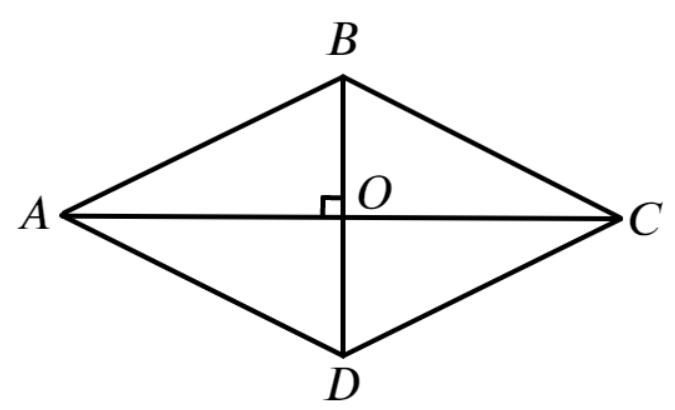
\includegraphics[scale=0.35]{g9-37.png}}
\end{figure}\\
В ромбе диагонали перпендикулярны и делятся точкой пересечения пополам. Поэтому \\$AB=\sqrt{49+576}=25$см. Найдём площадь ромба двумя способами, пусть его высота равна $h.$ С одной стороны, $S=\cfrac{1}{2}AC\cdot BD=\cfrac{1}{2}\cdot14\cdot48=336\text{ см}^2.$ С другой стороны, $S=h\cdot AB=25h.$ Значит,
$h=\cfrac{336}{25}\text{ см}.$\\
38. \begin{figure}[ht!]
\center{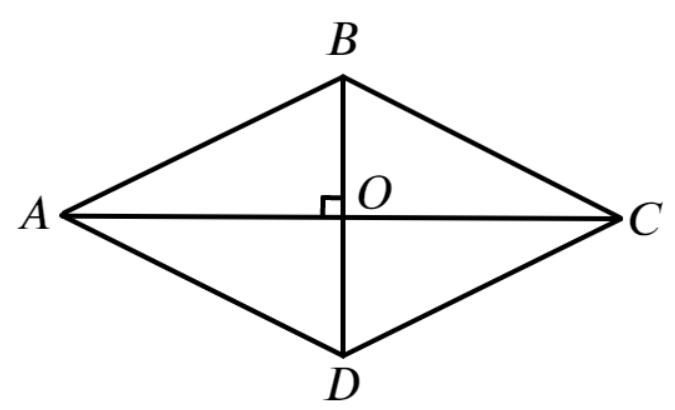
\includegraphics[scale=0.35]{g9-37.png}}
\end{figure}\\
В ромбе диагонали перпендикулярны и делятся точкой пересечения пополам. Поэтому \\$AB=\sqrt{25+144}=13$см. Найдём площадь ромба двумя способами, пусть его высота равна $h.$ С одной стороны, $S=\cfrac{1}{2}AC\cdot BD=\cfrac{1}{2}\cdot10\cdot24=120\text{ см}^2.$ С другой стороны, $S=h\cdot AB=13h.$ Значит,
$h=\cfrac{120}{13}\text{ см}.$\\
39. Сумма внешних углов любого многоугольника равна $360^\circ,$ а сумма его внутренних углов равна $(n-2)\cdot180^\circ,$ где $n$ это количество вершин. Значит, $(n-2)\cdot180^\circ=360^\circ,\ n=4.$\\
40. Сумма внешних углов любого многоугольника равна $360^\circ,$ а сумма его внутренних углов равна $(n-2)\cdot180^\circ,$ где $n$ это количество вершин. Значит, $(n-2)\cdot180^\circ=3\cdot360^\circ,\ n=8.$
ewpage


oindent41. \begin{figure}[ht!]
\center{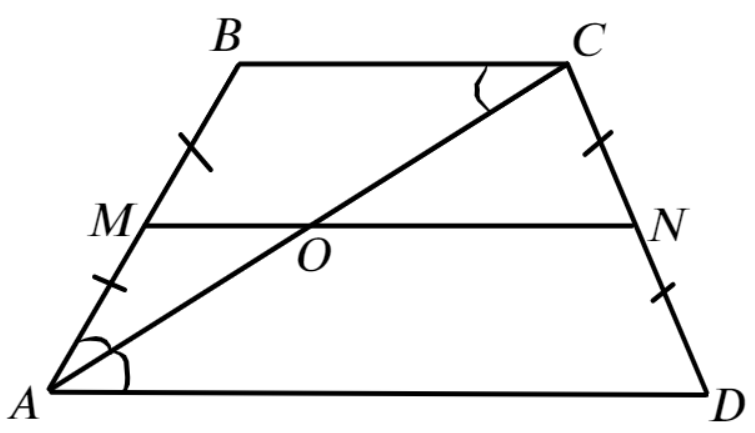
\includegraphics[scale=0.35]{g9-41.png}}
\end{figure}\\
Углы $BAC$ и $CAD$ равны так как $AC$ --- биссектриса, а углы $CAD$ и $BCA$ равны как накрест лежащие, значит $\angle BAC=\angle BCA$ и треугольник $ABC$ равнобедренный, $AB=BC.$ Прямая $MN$ параллельна основаниям трапеции и проходит через середины сторон $AB$ и $CD,$ значит отрезки $MO$ и $ON$ являются средними линиями треугольников $ABC$ и $ACD$ соответственно. Тогда $BC=2MO=2\cdot7,5=15$см и $AB=BC=CD=15$см (так как трапеция равнобедренная), а $AD=2AN=2\cdot12,5=25$см.\\
42. Раз трапеция описанная, суммы её противоположных сторон равны. Значит, сумма оснований равна $18:2=9$см. Тогда её средняя линия равна $9:2=4,5$см.\\
43. Углы при основании этого треугольника равны $(180^\circ-40^\circ):2=70^\circ.$ Тогда по теореме синусов имеем $\cfrac{20}{\sin(70^\circ)}=2R,\ R=\cfrac{10}{sin(70^\circ)}$см.\\
44. Угол при вершине этого треугольника равны $180^\circ-2\cdot30^\circ=120^\circ.$ Тогда по теореме синусов имеем $\cfrac{10}{\sin(120^\circ)}=2R,\ R=\cfrac{10\sqrt{3}}{3}$см.\\
45. \begin{figure}[ht!]
\center{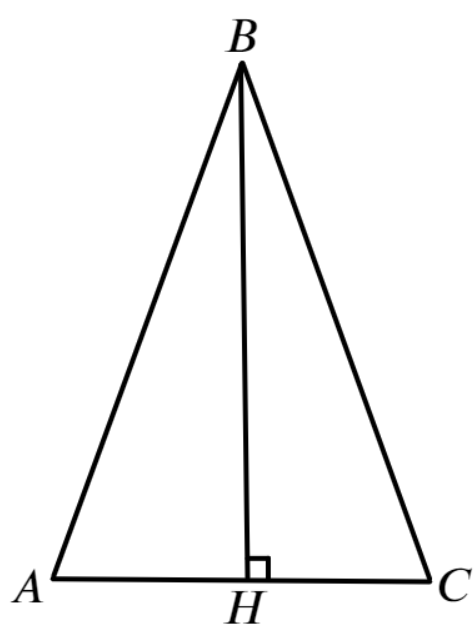
\includegraphics[scale=0.35]{g9-45.png}}
\end{figure}\\
Пусть боковая сторона треугольника равна $a,$ тогда по теореме косинусов $AC^2=a^2+a^2-2\cdot a\cdot a\cdot \cos(\angle B)=2a^2-\cfrac{14}{9}a^2=\cfrac{4}{9}a^2,$
тогда $AC=\cfrac{2}{3}a.$ Опустим из вершины высоту и медиану $BH,$ тогда $\cos(\angle A)=\cfrac{AH}{AB}=\cfrac{\cfrac{1}{3}a}{a}=\cfrac{1}{3},$
а $\sin(\angle A)=\sqrt{1-\cos^2(\angle A)}=\sqrt{1-\cfrac{1}{9}}=\cfrac{2\sqrt{2}}{3}.$
ewpage
oindent
46. \begin{figure}[ht!]
\center{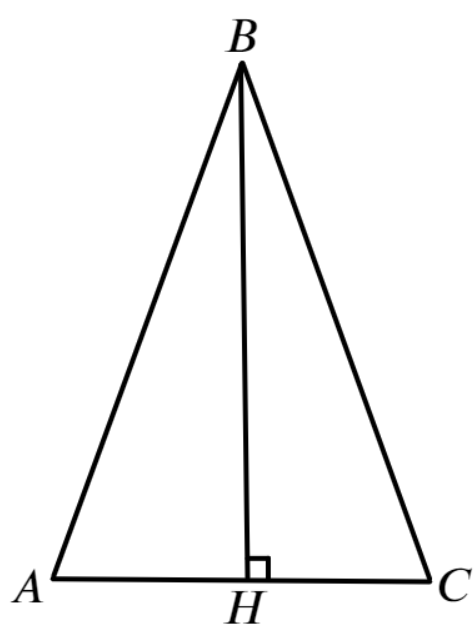
\includegraphics[scale=0.35]{g9-45.png}}
\end{figure}\\
Пусть боковая сторона треугольника равна $a,$ тогда по теореме косинусов $AC^2=a^2+a^2-2\cdot a\cdot a\cdot \cos(\angle B)=2a^2-\cfrac{10}{9}a^2=\cfrac{8}{9}a^2,$
тогда $AC=\cfrac{2\sqrt{2}}{3}a.$ Опустим из вершины высоту и медиану $BH,$ тогда $\cos(\angle A)=\cfrac{AH}{AB}=\cfrac{\cfrac{\sqrt{2}}{3}a}{a}=\cfrac{\sqrt{2}}{3},$
а $\sin(\angle A)=\sqrt{1-\cos^2(\angle A)}=\sqrt{1-\cfrac{2}{9}}=\cfrac{\sqrt{7}}{3}.$\\
47. \begin{figure}[ht!]
\center{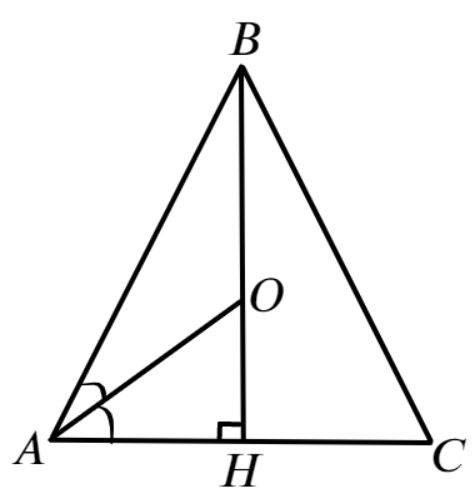
\includegraphics[scale=0.35]{g9-47.png}}
\end{figure}\\
Центр вписанного круга --- это точка пересечения биссектрис треугольника, значит делить он может только высоту, опущенную из вершины (совпадающую с биссектрисой). По свойству основания биссектрисы имеем соотношение $\cfrac{AB}{AH}=\cfrac{BO}{OH}.$ Возможны два случая: $\cfrac{60}{AH}=\cfrac{12}{5},\ AH=25,\ AC=50$см или
$\cfrac{60}{AH}=\cfrac{5}{12},\ AH=144,\ AC=288$см.\\
48. Выразим площадь треугольника двумя способами: $S=pr=\cfrac{1}{2}ha,$ значит $28\cdot\cfrac{2}{7}h=\cfrac{1}{2}ha,\ a=16$см. Если сторона $a$ является основанием, то стороны треугольника равны 16 см, $(56-16):2=20$см и 20 см, а если она является боковой стороной, то 16 см, 16 см и $56-2\cdot16=24$см.\\
49. \begin{figure}[ht!]
\center{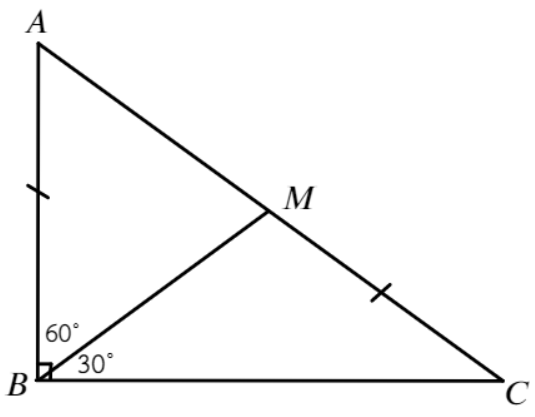
\includegraphics[scale=0.35]{g9-49.png}}
\end{figure}\\
Из теорем синусов для треугольников $AMB$ и $CMB$ получим равенства\\ $\cfrac{AB}{\sin(AMB)}=\cfrac{AM}{\sin(60^\circ)},\ \cfrac{BC}{\sin(\angle BMC)}= \cfrac{MC}{\sin(30^\circ)}.$ Так как синусы смежных углов равны, после деления равенств друг на друга получим соотношение $\cfrac{AB}{BC}=\cfrac{AM\cdot\cfrac{1}{2}}{MC\cdot\cfrac{\sqrt{3}}{2}},$ откуда $AM\cdot BC=4\sqrt{3}.$ Пусть $BC=x,$ тогда $AM=\cfrac{4\sqrt{3}}{x}.$ По теореме Пифагора имеем $x^2+4=\left(\cfrac{4\sqrt{3}}{x}+2
ight)^2,\ x^2+4=\cfrac{48}{x^2}+\cfrac{16\sqrt{3}}{x}+4,\ x^4-16\sqrt{3}x-48=0,\ x^4-2\sqrt{3}x^3+2\sqrt{3}x^3-12x^2+12x^2-24\sqrt{3}x+8\sqrt{3}x-48=0,$\\
$x^3(x-2\sqrt{3})+2\sqrt{3}x^2(x-2\sqrt{3})+12x(x-2\sqrt{3})+8\sqrt{3}(x-2\sqrt{3})=0,\ (x-2\sqrt{3})(x^3+2\sqrt{3}x^2+12x+8\sqrt{3})=0,\ x=2\sqrt{3}$см. Решение единственно, так как $x>0.$\\
50. \begin{figure}[ht!]
\center{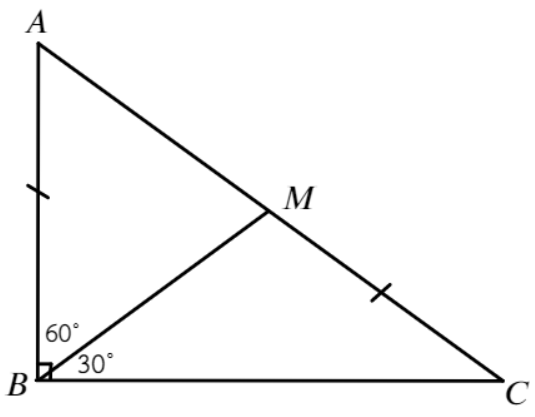
\includegraphics[scale=0.35]{g9-49.png}}
\end{figure}\\
Из теорем синусов для треугольников $AMB$ и $CMB$ получим равенства\\ $\cfrac{AB}{\sin(AMB)}=\cfrac{AM}{\sin(60^\circ)},\ \cfrac{BC}{\sin(\angle BMC)}= \cfrac{MC}{\sin(30^\circ)}.$ Так как синусы смежных углов равны, после деления равенств друг на друга получим соотношение $\cfrac{AB}{BC}=\cfrac{AM\cdot\cfrac{1}{2}}{MC\cdot\cfrac{\sqrt{3}}{2}},$ откуда $AM\cdot BC=9\sqrt{3}.$ Пусть $BC=x,$ тогда $AM=\cfrac{9\sqrt{3}}{x}.$ По теореме Пифагора имеем $x^2+9=\left(\cfrac{9\sqrt{3}}{x}+3
ight)^2,\ x^2+9=\cfrac{243}{x^2}+\cfrac{54\sqrt{3}}{x}+9,\ x^4-54\sqrt{3}x-243=0,\ x^4-3\sqrt{3}x^3+3\sqrt{3}x^3-27x^2+27x^2-81\sqrt{3}x+27\sqrt{3}x-243=0,$\\
$x^3(x-3\sqrt{3})+3\sqrt{3}x^2(x-3\sqrt{3})+27x(x-3\sqrt{3})+27\sqrt{3}(x-3\sqrt{3})=0,\ (x-3\sqrt{3})(x^3+3\sqrt{3}x^2+27x+27\sqrt{3})=0,\ x=3\sqrt{3}$см. Решение единственно, так как $x>0.$\\
51. \begin{figure}[ht!]
\center{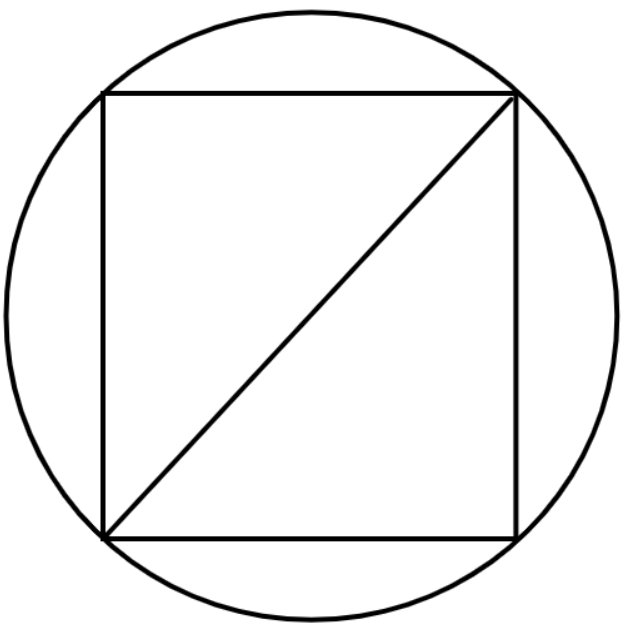
\includegraphics[scale=0.35]{g9-51.png}}
\end{figure}\\
Так как прямой угол опирается на диаметр, диагональ квадрата равна диаметру окружности, а значит она равна $2\cdot\sqrt{12}=4\sqrt{3}.$ Углы равностороннего треугольника равны по $60^\circ,$ найдём радиус искомой окружности по теореме синусов: $\cfrac{4\sqrt{3}}{\sin(60^\circ)}=2R,\ R=4.$
ewpage
oindent
52. \begin{figure}[ht!]
\center{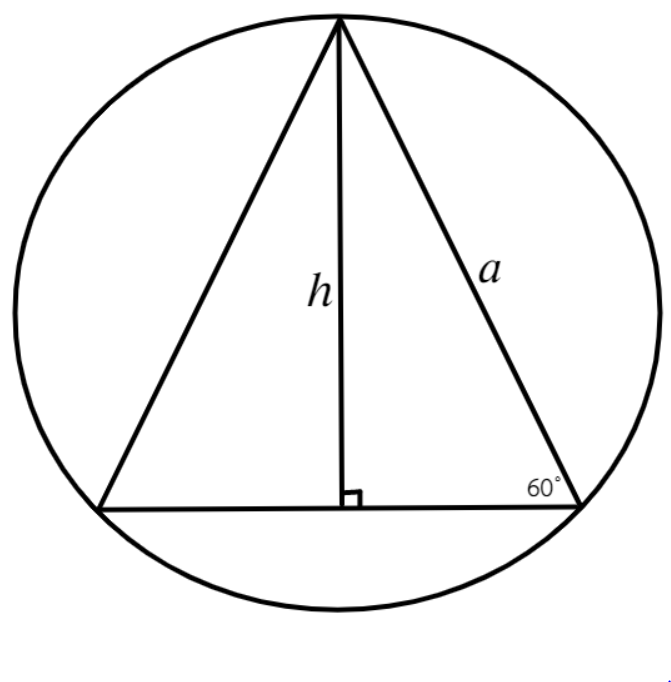
\includegraphics[scale=0.35]{g9-52.png}}
\end{figure}\\
Пусть сторона правильно треугольника равна $a,$ а высота $h.$ По теореме синусов имеем соотношение $\cfrac{a}{\sin(60^\circ)}=2R,\ a=\cfrac{\sqrt{3}}{2}\cdot\sqrt{12},\ a=3.$ Тогда высота $h=a\sin(60^\circ)=3\cdot\cfrac{\sqrt{3}}{2}=\cfrac{3\sqrt{3}}{2}.$ Радиус вписанной окружности равностороннего треугольника можно найти по формуле $r=\cfrac{h}{2}tg(30^\circ)=\cfrac{3\sqrt{3}}{4}\cdot\cfrac{\sqrt{3}}{3}=\cfrac{3}{4}.$\\
53. \begin{figure}[ht!]
\center{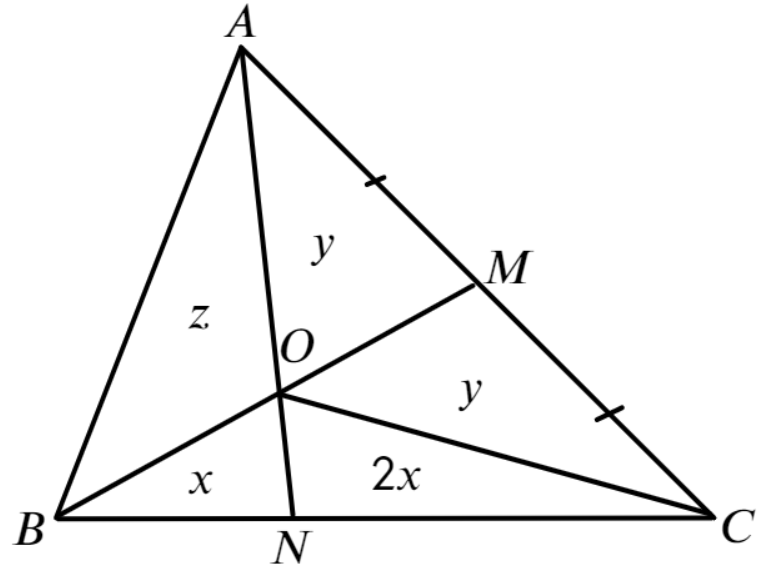
\includegraphics[scale=0.35]{g9-53.png}}
\end{figure}\\
Воспользовавшись тем, что площади треугольников, имеющих общую высоту, относятся как основания, на которые она опущена, введём обозначения: $S_{\Delta OBN}=x,\ S_{\Delta OCN}=2x,\ S_{\Delta AOM}=S_{\Delta COM}=y,\ S_{\Delta AOB}=z.$ Тогда так как $S_{\Delta ABM}=S_{\Delta CBM},$ имеем равенство $z+y=3x+y,$ откуда $z=3x.$ Так как $S_{\Delta ACN}=2S_{\Delta ABN},$ получим соотношения $(3x+x)\cdot2=2y+2x,\ y=3x.$ Так как $S_{\Delta ABO}=S_{\Delta AOM}=3x,$ получаем $BO:OM=1:1,$ а так как $\cfrac{S_{\Delta ABO}}{S_{\Delta BON}}=3,$ получаем $AO:ON=3:1.$\\
54. \begin{figure}[ht!]
\center{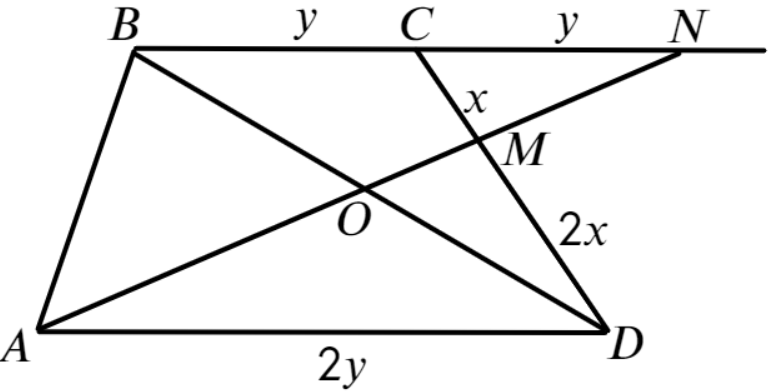
\includegraphics[scale=0.35]{g9-54.png}}
\end{figure}\\
Обозначим $CM=x,\ DM=2x,\ BC=y,\ AD=2y.$ Продлим $AM$ до пересечения с продолжением $BC$ в точке $N.$ Треугольники $CMN$ и $AMD$ подобны по двум углам (накрест лежащие  $MCN$ с $MDA$ и $MNC$ с $MAD$, значит $\cfrac{CN}{AD}=\cfrac{CM}{DM}=\cfrac{1}{2},\ CN=y.$ Тогда $BN=y+y=2y=AD$ и треугольники $OBN$ и $ODA$ равны по стороне и двум прилежащим к ней углам (накрест лежащие $OBN$ с $ODA$ и $ONB$ с $OAD),$ поэтому $BO=OD$ и $BO:OD=1:1,$ а также $AO=ON.$ Из подобия треугольников $CMN$ и $AMD$ получаем $AM=2MN.$ Значит, $MN=\cfrac{1}{3}AN,$ а $AO=\cfrac{1}{2}AN,$ поэтому $OM=AN-AO-MN=\cfrac{1}{6}AN.$ Таким образом, $AO:OM=\cfrac{1}{2}AN:\cfrac{1}{6}AN=3:1.$\\
55. Так как перпендикуляр короче наклонной, у такого треугольника есть две стороны, большие 1 м. Значит, хотя бы на одну из них опущена высота, большая 1 м (иначе сторон треугольника было бы 4), а тогда его площадь хотя бы $\cfrac{1}{2}\cdot1\cdot1=0,5\text{ м}^2$ и не может быть равна $1\text{см}^2.$\\
56. \begin{figure}[ht!]
\center{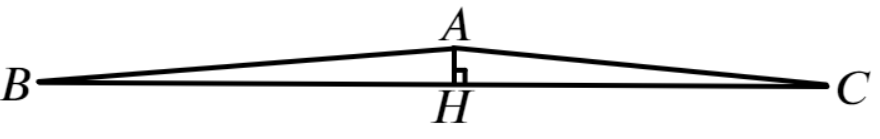
\includegraphics[scale=0.35]{g9-56.png}}
\end{figure}\\
Рассмотрим равнобедренный треугольник $ABC,$ у которого $AB=AC=2$м, а высота $AH=0,00001$м. Тогда по неравенству треугольника $BC<AB+AC=4$м, а площадь $S=\cfrac{1}{2}AH\cdot BC<\cfrac{1}{2}\cdot0,00001\cdot4=0,00002\text{ м}^2.$ Значит, такой треугольник существует.\\
57. а) Так как равные хорды стягивают равные дуги, каждый угол многоугольника опирается на дугу одной и той же длины, поэтому все углы равны, утверждение верно.\\
б) Утверждение неверно, в качестве контрпримера можно рассмотреть любой прямоугольник (он вписан, так как сумма противоположных углов равна $180^\circ$), не являющийся квадратом.\\
58. а) Утверждение неверно, в качестве примера можно рассмотреть любой ромб (он описан, так как суммы противоположных сторон равны), не являющийся квадратом.\\
б) \begin{figure}[ht!]
\center{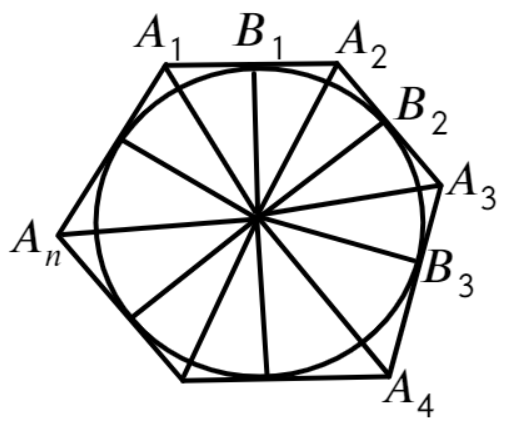
\includegraphics[scale=0.35]{g9-58.png}}
\end{figure}\\
Пусть углы многоугольника равны $\alpha.$ Соединим центр окружности $O$ со всеми вершинами и со всеми точками касания. Треугольники $OB_1A_2$ и $OB_2A_2$ равны по катету и гипотенузе, значит $B_1A_2=B_2A_2$ и $\angle B_1A_2O=\angle B_2A_2O=\cfrac{\alpha}{2}.$ Треугольники $OB_2A_3$ и $OB_3A_3$ также равны по катету и гипотенузе, значит $B_2A_3=B_3A_3$ и $\angle B_2A_3O=\angle B_3A_3O=\cfrac{\alpha}{2}.$ Но тогда треугольники $OA_2B_2$ и $OA_3B_2$ равны по катету и острому углу, поэтому $B_2A_2=B_2A_3.$ Проведя аналогичные рассуждения необходимое количество раз, получим, что все отрезки, на которые точки касания разбивают стороны, равны, а значит равны все стороны многоугольника, утверждение является верным.\\
59. По теореме Пифагора половина основания равна $\sqrt{13^2-5^2}=12,$ тогда основание равно $12\cdot2=24.$ Тогда площадь этого треугольника равна $S=\cfrac{1}{2}\cdot5\cdot24=60.$ С другой стороны она равна $rp,$ где $p=\cfrac{13+13+24}{2}=25.$ Поэтому радиус вписанной окружности равен $60:25=2,4.$ Также площадь треугольника можно найти по формуле $S=\cfrac{abc}{4R}=\cfrac{13\cdot13\cdot24}{4R}=\cfrac{169\cdot6}{R}.$ Поэтому радиус описанной окружности равен $\cfrac{169\cdot6}{60}=16,9.$
ewpage
oindent
60. \begin{figure}[ht!]
\center{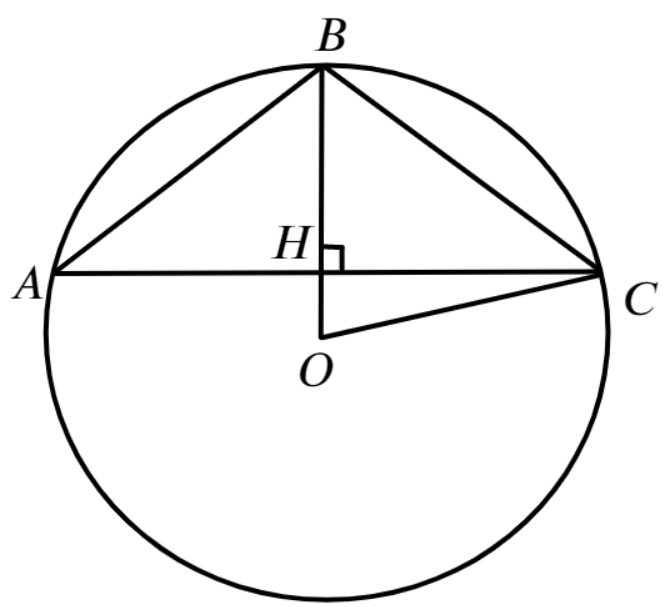
\includegraphics[scale=0.35]{g9-60.png}}
\end{figure}\\
Центр описанной окружности тупоугольного треугольника лежит снаружи. Найдём $BH=BO-OH=2-1=1$ и $HC=\sqrt{2^2-1^2}=\sqrt{3},\ AC=2HC=2\sqrt{3}.$ Тогда $S=\cfrac{1}{2}\cdot1\cdot2\sqrt{3}=\sqrt{3}.$ Выразим $AB=BC=\sqrt{1^2+(\sqrt{3})^2}=2.$ Площадь также можно найти по формуле $S=pr=\cfrac{2+2+2\sqrt{3}}{2}r=(2+\sqrt{3})r.$ Значит, $r=\cfrac{\sqrt{3}}{2+\sqrt{3}}=\cfrac{\sqrt{3}(2-\sqrt{3})}{4-3}=2\sqrt{3}-3.$\\
61. \begin{figure}[ht!]
\center{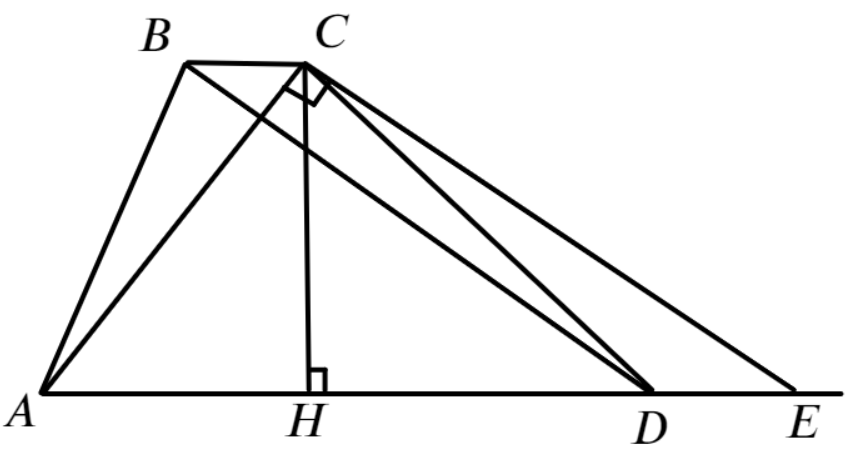
\includegraphics[scale=0.35]{g9-61.png}}
\end{figure}\\
Пусть диагональ $BD=5.$ Проведём через вершину $C$ прямую, параллельную $BD,$ точку её пересечения с прямой $AD$ обозначим буквой $E.$ Тогда $BCED$ является параллелограммом, а значит $CE=BD=5.$ Так как $AC\perp BD,$ то и $AC\perp CE.$ Опустим высоту $CH,$ тогда $HE=\sqrt{5^2-4^2}=3.$ Треугольники $ACH$ и $CHE$ подобны по двум углам ($\angle HCE=90^\circ-\angle HEC=\angle HAC,\ \angle CHE=90^\circ=\angle AHC$), значит $\cfrac{AC}{CE}=\cfrac{CH}{HK},\ \cfrac{AC}{5}=\cfrac{4}{3},\ AC=\cfrac{20}{3}.$ Тогда $S_{ABCD}=\cfrac{1}{2}CH\cdot(BC+AD)=\cfrac{1}{2}CH\cdot AE=S_{\Delta ACE}=\cfrac{AC\cdot CE}{2}=\cfrac{50}{3}.$\\
62. \begin{figure}[ht!]
\center{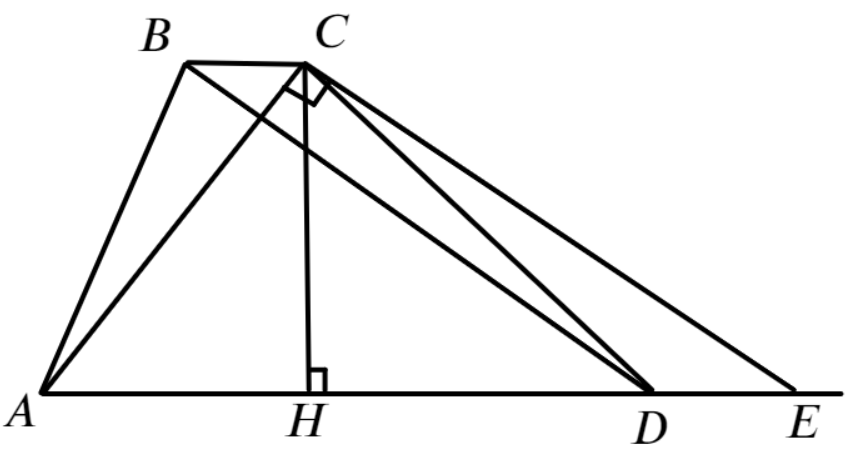
\includegraphics[scale=0.35]{g9-61.png}}
\end{figure}\\
Пусть диагональ $BD=5.$ Проведём через вершину $C$ прямую, параллельную $BD,$ точку её пересечения с прямой $AD$ обозначим буквой $E.$ Тогда $BCED$ является параллелограммом, а значит $CE=BD=5$ и $BC=DE,$ а значит $AE=AD+DE=AD+BC=2\cdot6,5=13.$ Так как $AC\perp BD,$ то и $AC\perp CE.$
Опустим высоту $CH,$ тогда $S_{ABCD}=\cfrac{1}{2} CH\cdot (AD+BC)=\cfrac{1}{2} CH\cdot AE=S_{\Delta ACE}.$ Найдём $AC=\sqrt{13^2-5^2}=12,$ тогда $S_{\Delta ACE}=\cfrac{12\cdot5}{2}=30.$\\
63. \begin{figure}[ht!]
\center{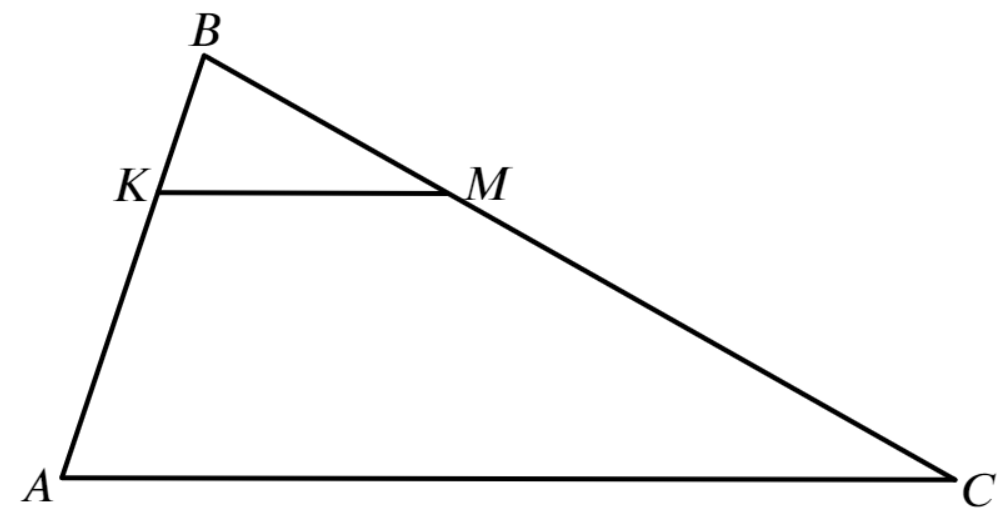
\includegraphics[scale=0.35]{g9-63.png}}
\end{figure}\\
Пусть $BK=2x,$ тогда $KA=5x,\ AB=7x.$ Треугольники $ABC$ и $KBM$ подобны по двум углам (соответственные $BAC$ с $BKM$ и $BCA$ с $BMK$), значит $\cfrac{AC}{KM}=\cfrac{AB}{BK},\ \cfrac{21}{KM}=\cfrac{7x}{2x},\ KM=6$см.\\
64. \begin{figure}[ht!]
\center{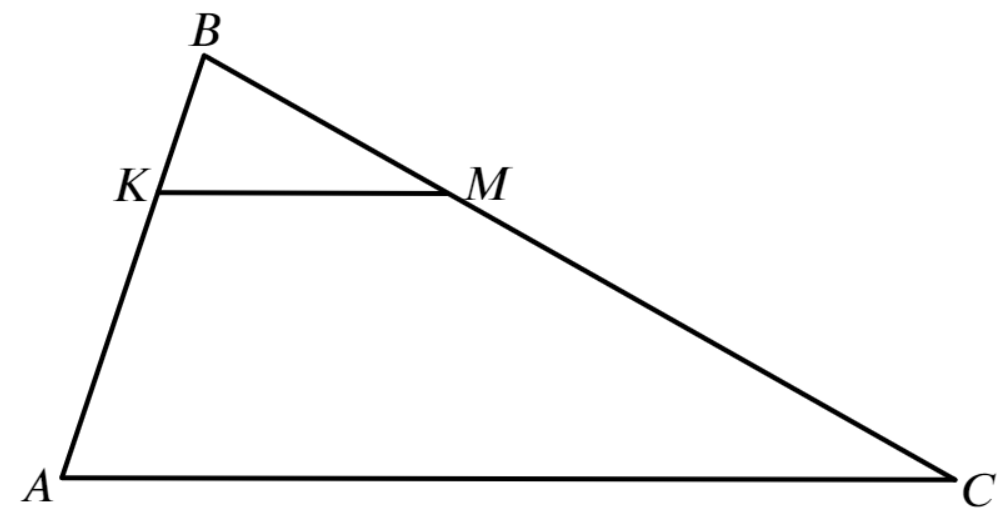
\includegraphics[scale=0.35]{g9-63.png}}
\end{figure}\\
Пусть $BK=3x,$ тогда $KA=4x,\ AB=7x.$ Треугольники $ABC$ и $KBM$ подобны по двум углам (соответственные $BAC$ с $BKM$ и $BCA$ с $BMK$), значит $\cfrac{AC}{KM}=\cfrac{AB}{BK},\ \cfrac{AC}{18}=\cfrac{7x}{3x},\ AC=42$см.\\
65. Координаты точки $M$ являются средним арифметическим координат точек $A$ и $C:$\\$ \left(\cfrac{2+4}{2}; \cfrac{5+3}{2}
ight)=(3;4).$ Тогда длина $BM$ равна $\sqrt{(3-0)^2+(4-0)^2}=5.$\\
66. Координаты точки $M$ являются средним арифметическим координат точек $A$ и $C:$\\$ \left(\cfrac{-3+0}{2}; \cfrac{-2+0}{2}
ight)=(-1,5;-1).$ Тогда длина $BM$ равна $\sqrt{(-1,5+6)^2+(-1-2)^2}=\cfrac{3\sqrt{13}}{2}.$\\
67. \begin{figure}[ht!]
\center{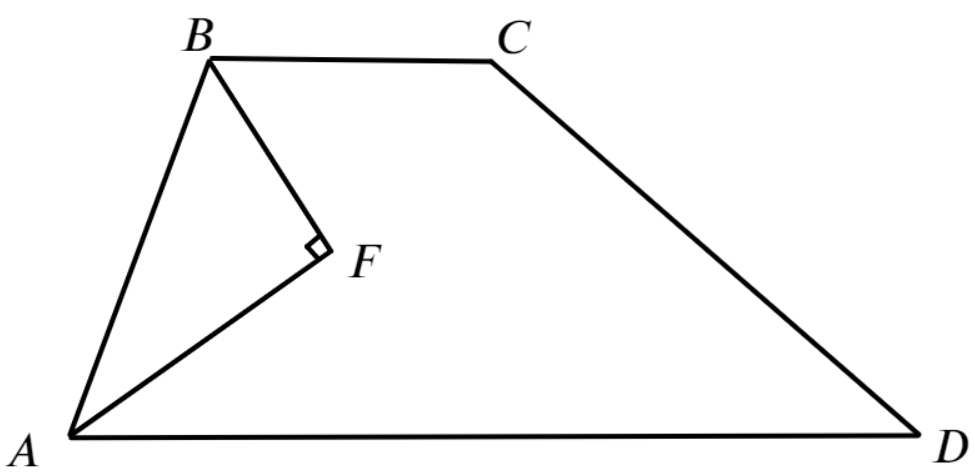
\includegraphics[scale=0.35]{g9-67.png}}
\end{figure}\\
Углы $A$ и $B$ являются односторонними, значит $\angle A+\angle B=180^\circ,$ поэтому $\angle BAF+\angle ABF=\cfrac{1}{2}(\angle A+\angle B)=90^\circ$ и $\angle AFB=180^\circ-90^\circ=90^\circ.$ Тогда по теореме Пифагора получаем $AB=\sqrt{24^2+10^2}=26$см.
ewpage
oindent
68. \begin{figure}[ht!]
\center{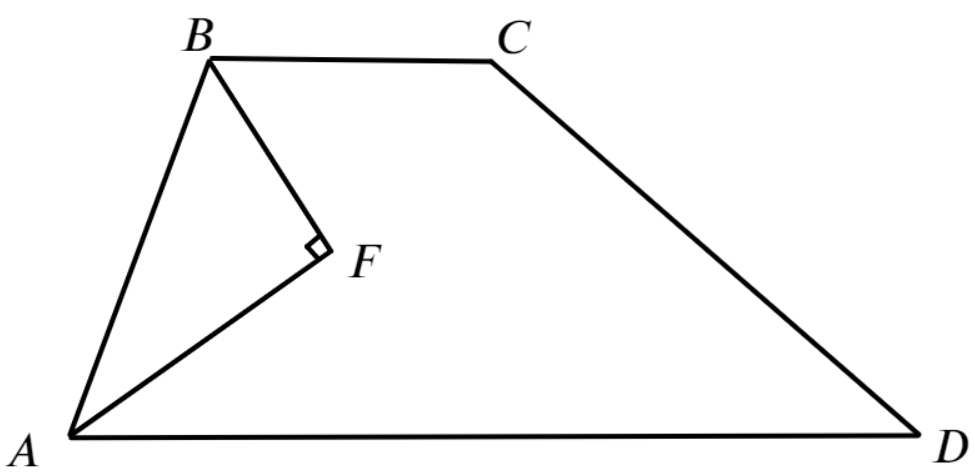
\includegraphics[scale=0.35]{g9-67.png}}
\end{figure}\\
Углы $A$ и $B$ являются односторонними, значит $\angle A+\angle B=180^\circ,$ поэтому $\angle BAF+\angle ABF=\cfrac{1}{2}(\angle A+\angle B)=90^\circ$ и $\angle AFB=180^\circ-90^\circ=90^\circ.$ Тогда по теореме Пифагора получаем $AB=\sqrt{24^2+18^2}=30$см.\\
69. \begin{figure}[ht!]
\center{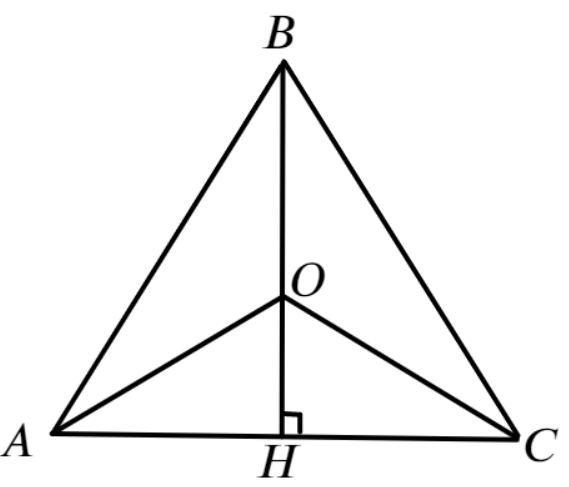
\includegraphics[scale=0.35]{g9-69.png}}
\end{figure}\\
Проведём из вершины высоту $BH$ и отметим на ней центр описанной окружности $O$ (высота является серединным перпендикуляром, поэтому он ей принадлежит). Тогда $OH=BH-BO=8-5=3,\ HC=\sqrt{5^2-3^2}=4,\ AC=2HC=8,\ S_{\Delta ABC}=\cfrac{1}{2}\cdot8\cdot8=32\text{ см}^2.$\\
70. \begin{figure}[ht!]
\center{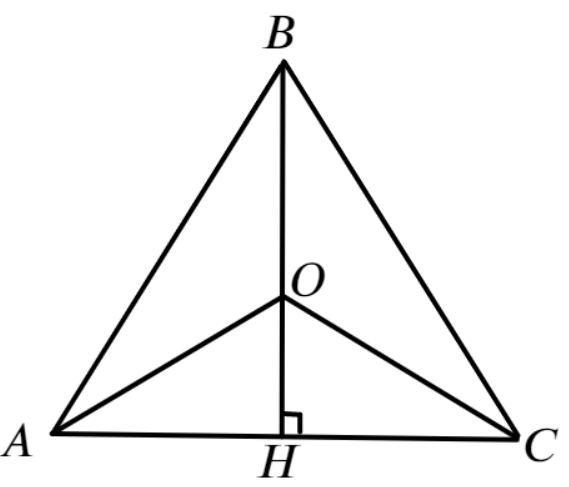
\includegraphics[scale=0.35]{g9-69.png}}
\end{figure}\\
Проведём из вершины высоту $BH$ и отметим на ней центр описанной окружности $O$ (высота является серединным перпендикуляром, поэтому он ей принадлежит). Тогда $HC=AC:2=6,\ OH=\sqrt{10^2-6^2}=8,\ BH=8+10=18,\ S_{\Delta ABC}=\cfrac{1}{2}\cdot18\cdot12=108\text{ см}^2.$\\
71. \begin{figure}[ht!]
\center{\includegraphics[scale=0.35]{g9-71.png}}
\end{figure}\\
По свойству основания биссектрисы имеем соотношение $\cfrac{AB}{AC}=\cfrac{BM}{MC}=3:1.$ Пусть $AC=x,\ AB=3x,$ тогда по теореме Пифагора $x^2+9x^2=(3+1)^2,\ x^2=\cfrac{8}{5}.$ Посчитаем площадь треугольника двумя способами: $S=\cfrac{1}{2}AD\cdot4=\cfrac{1}{2}x\cdot3x,$ откуда $4AD=3\cdot\cfrac{8}{5},\ AD=\cfrac{6}{5}.$\\
72. \begin{figure}[ht!]
\center{\includegraphics[scale=0.35]{g9-72.png}}
\end{figure}\\
По свойству основания биссектрисы имеем соотношение $\cfrac{AB}{AC}=\cfrac{BM}{MC}=2:4=1:2.$ Пусть $AB=x,\ AC=2x,$ тогда по теореме Пифагора $x^2+4x^2=(2+4)^2,\ x^2=\cfrac{36}{5}.$ Посчитаем площадь треугольника двумя способами: $S=\cfrac{1}{2}AD\cdot6=\cfrac{1}{2}x\cdot2x,$ откуда $6AD=2\cdot\cfrac{36}{5},\ AD=\cfrac{12}{5}.$\\
73. Пусть боковая сторона равна $x,$ тогда по теореме косинусов имеем равенство $x^2+x^2-2x\cdot x\cdot \cos\left(\cfrac{\pi}{4}
ight)=1^2,$ откуда $x^2(2-\sqrt{2})=1,\ x^2=\cfrac{1}{2-\sqrt{2}}=\cfrac{2+\sqrt{2}}{4-2}=\cfrac{2+\sqrt{2}}{2}.$ Тогда сумма квадратов всех сторон равна $2x^2+1=2+\sqrt{2}+1=3+\sqrt{2}.$\\
74. Пусть боковая сторона равна $x,$ тогда по теореме косинусов имеем равенство $x^2+x^2-2x\cdot x\cdot \cos\left(\cfrac{\pi}{6}
ight)=1^2,$ откуда $x^2(2-\sqrt{3})=1,\ x^2=\cfrac{1}{2-\sqrt{3}}=\cfrac{2+\sqrt{3}}{4-3}=2+\sqrt{3}.$ Тогда сумма квадратов всех сторон равна $2x^2+1=4+2\sqrt{3}+1=5+2\sqrt{3}.$\\
75. \begin{figure}[ht!]
\center{\includegraphics[scale=0.35]{g9-75.png}}
\end{figure}\\
Пусть $AB=BC=CD=1$см, $AD=2$см. Опустим высоту $BH.$ Так как трапеция равнобедренная, $AH=(2-1):2=\cfrac{1}{2},\ BH=\sqrt{1-\cfrac{1}{4}}=\cfrac{\sqrt{3}}{2}.$ Тогда $BD=\sqrt{\cfrac{3}{4}+\left(2-\cfrac{1}{2}
ight)^2}=\sqrt{3}, \sin(\angle BDH)=\cfrac{\cfrac{\sqrt{3}}{2}}{\sqrt{3}}=\cfrac{1}{2}.$ Окружность, описанная вокруг трапеции $ABCD,$ описана также и вокруг треугольника $ABD,$ поэтому по теореме синусов получаем $\cfrac{AB}{\sin(\angle BDH)}=2R,\ \cfrac{1}{\cfrac{1}{2}}=2R,\ R=1$см.\\
76. Вычислим $\sin(\angle C)=\sqrt{1-\cfrac{2}{4}}=\cfrac{\sqrt{2}}{2}.$ Найдём площадь треугольника двумя способами: $S=\cfrac{1}{2}AH\cdot 2\sqrt{2}=\cfrac{1}{2}\cdot\cfrac{\sqrt{2}}{2}\cdot 2\sqrt{2}\cdot2\sqrt{2},$ откуда $AH=2.$
ewpage
oindent
77. Вычислим $\sin(\angle A)=\sqrt{1-\cfrac{7}{16}}=\cfrac{3}{4}.$ Найдём площадь треугольника двумя способами: $S=\cfrac{1}{2}BH\cdot AC=\cfrac{1}{2}\cdot\cfrac{3}{4}\cdot AC\cdot8,$ откуда $BH=6.$\\
78. Координаты точки $M$ являются средним арифметическим координат точек $A$ и $C:$\\$ \left(\cfrac{1+4}{2}; \cfrac{4+1}{2}
ight)=\left(\cfrac{5}{2};\cfrac{5}{2}
ight).$ Тогда длина $BM$ равна $\sqrt{\left(\cfrac{5}{2}-0
ight)^2+\left(\cfrac{5}{2}-0
ight)^2}=\cfrac{5\sqrt{2}}{2}.$\\
79. Координаты точки $M$ являются средним арифметическим координат точек $A$ и $C:$\\$ \left(\cfrac{3+0}{2}; \cfrac{2+0}{2}
ight)=\left(\cfrac{3}{2};1
ight).$ Тогда длина $BM$ равна $\sqrt{\left(\cfrac{3}{2}-2
ight)^2+\left(1-3
ight)^2}=\cfrac{\sqrt{17}}{2}.$\\
80. \begin{figure}[ht!]
\center{\includegraphics[scale=0.35]{g9-80.png}}
\end{figure}\\
Найдём $\angle B=90^\circ-24^\circ=66^\circ.$ Тогда $\angle BCH=90^\circ-66^\circ=24^\circ.$ Медиана, проведённая из прямого угла, равна половине гипотенузы, поэтому $CM=MA,$ а значит $\angle MCA=\angle A=24^\circ.$ Таким образом, $\angle HCM=90^\circ-24^\circ-24^\circ=42^\circ.$\\
81. \begin{figure}[ht!]
\center{\includegraphics[scale=0.35]{g9-81.png}}
\end{figure}\\
Найдём $\angle B=90^\circ-53^\circ=37^\circ$ и $\angle ACH=90^\circ-53^\circ=37^\circ.$ Медиана, проведённая из прямого угла, равна половине гипотенузы, поэтому $CM=MB,$ а значит $\angle MCB=\angle B=37^\circ.$ Таким образом, $\angle HCM=90^\circ-37^\circ-37^\circ=16^\circ.$\\
82. \begin{figure}[ht!]
\center{\includegraphics[scale=0.35]{g9-82.png}}
\end{figure}\\
$\sin(\angle B)=\cfrac{CH}{BC}=\cfrac{CH}{AD}=\cfrac{20}{25}=\cfrac{4}{5}.$
ewpage
oindent
83. \begin{figure}[ht!]
\center{\includegraphics[scale=0.35]{g9-82.png}}
\end{figure}\\
$\sin(\angle B)=\cfrac{CH}{BC}=\cfrac{CH}{AD}=\cfrac{14}{28}=\cfrac{1}{2}.$\\
84. \begin{figure}[ht!]
\center{\includegraphics[scale=0.35]{g8-169.png}}
\end{figure}\\
Отложим на отрезке $OC$ точку $C'$ так, чтобы $AO=OC'$ (это можно сделать, так как $AO<OC$). Тогда в четырёхугольнике $ABC'D$ диагонали делятся точкой пересечения пополам, значит он является параллелограммом и $\angle BC'D=\angle BAD.$ Углы $BC'O$ и $DC'O$ являются внешними в треугольниках $BC'C$ и $DC'C,$ поэтому $\angle BAD=\angle BC'D=\angle BC'O+\angle DC'O=\angle C'BC+\angle C'CB+\angle C'DC+\angle C'CD=\angle BCD+\angle C'BC+\angle C'DC>\angle BCD,$ ч.т.д.\\
85. \begin{figure}[ht!]
\center{\includegraphics[scale=0.35]{g8-172.png}}
\end{figure}\\
а) Опустим высоты $BB_1$ и $CC_1.$ Пусть высота трапеции равна $x,$ тогда $AB_1=x\ ctg(60^\circ)=\cfrac{\sqrt{3}}{3}x,\ C_1D=x\ ctg(30^\circ)=\sqrt{3}x,$ значит $a=
\cfrac{\sqrt{3}}{3}x+b+\sqrt{3}x,\ \cfrac{4\sqrt{3}}{3}x=a-b,\ x=\cfrac{3(a-b)}{4\sqrt{3}}=\cfrac{\sqrt{3}(a-b)}{4}.$ Тогда
$S_{ABCD}=\cfrac{\sqrt{3}(a-b)}{4}\cdot\cfrac{a+b}{2}=\cfrac{\sqrt{3}(a^2-b^2)}{8}.$\\
б) Продлим боковые стороны трапеции до пересечения, тогда точка их пересечения лежит на одной прямой с серединами оснований (и с точкой пересечения диагоналей, но в нашей задаче это не требуется). Тогда $\angle AED=180^\circ-30^\circ-60^\circ=90^\circ.$ Отрезки $EN$ и $EM$ являются медианами, проведёнными из прямого угла, значит $MN=EN-EM=\cfrac{1}{2}AD-\cfrac{1}{2}BC=\cfrac{1}{2}(AD-BC)=\cfrac{a-b}{2}.$\\
86. Раз трапеция вписанная, она равнобедренная. Сумму оснований равна удвоенной длине средней линии, то есть $5\cdot2=10.$ Тогда боковые стороны равны $(22-10):2=6.$
ewpage
oindent
87. \begin{figure}[ht!]
\center{\includegraphics[scale=0.35]{g9-87.png}}
\end{figure}\\
Пусть $AB=BC=CD=x,$ тогда $2x\cos(60^\circ)+x=12,\ 2x=12,\ x=6.$ Найдём $AH=(12-6):2=3,\ BH=3tg(60^\circ)=3\sqrt{3},\ HD=12-3=9,\ BD=\sqrt{27+81}=6\sqrt{3}.$ Описанная вокруг трапеции $ABCD$ окружность является также и описанной окружностью треугольника $ABD,$ значит по теореме синусов $\cfrac{BD}{\sin(60^\circ)}=2R,\ \cfrac{6\sqrt{3}}{\cfrac{\sqrt{3}}{2}}=2R,\ R=6.$\\
88. $S=\cfrac{1}{2}\cdot10\cdot10\cdot \sin(30^\circ)=25.$\\
89. $S=\cfrac{1}{2}\cdot20\cdot20\cdot \sin(150^\circ)=100.$\\
90. \begin{figure}[ht!]
\center{\includegraphics[scale=0.35]{g9-90.png}}
\end{figure}\\
Рассматриваемый треугольник является прямоугольным, поэтому центр его описанной окружности --- это середина гипотенузы. Её абсцисса равна $(8+0):2=4.$\\
91. \begin{figure}[ht!]
\center{\includegraphics[scale=0.35]{g9-90.png}}
\end{figure}\\
Рассматриваемый треугольник является прямоугольным, поэтому центр его описанной окружности --- это середина гипотенузы. Её ордината равна $(6+0):2=3.$
ewpage
oindent
92. \begin{figure}[ht!]
\center{\includegraphics[scale=0.35]{g9-92.png}}
\end{figure}\\
Продолжим $MB_1$ так, чтобы $MB_1=B_1D.$ Тогда в четырёхугольнике $AMCD$ диагонали делятся точкой пересечения пополам, а значит он является параллелограммом и $CD=AM.$ Так как медианы делятся точкой пересечения $M$ в отношении $2:1,$ считая от вершины, стороны треугольника $CMD$ равны $2,\ \cfrac{8}{3}$ и $\cfrac{10}{3}.$ Так как $2^2+\left(\cfrac{8}{3}
ight)^2=\left(\cfrac{10}{3}
ight)^2,$ этот треугольник является прямоугольным и  $S_{\Delta CMD}=\cfrac{2\cdot\cfrac{8}{3}}{2}=\cfrac{8}{3},\ S_{AMCD}=2S_{\Delta CMD}=\cfrac{16}{3},\ S_{\Delta AMC}=\cfrac{1}{2}S_{ABCD}=\cfrac{8}{3}.$ Так как медианы делят любой треугольник на 6 равновеликих, $S_{\Delta ABC}=3S_{\Delta AMC}=8.$\\
93. \begin{figure}[ht!]
\center{\includegraphics[scale=0.35]{g9-92.png}}
\end{figure}\\
Продолжим $MB_1$ так, чтобы $MB_1=B_1D.$ Тогда в четырёхугольнике $AMCD$ диагонали делятся точкой пересечения пополам, а значит он является параллелограммом и $CD=AM.$ Так как медианы делятся точкой пересечения $M$ в отношении $2:1,$ считая от вершины, стороны треугольника $CMD$ равны $8,\ 10$ и $14.$ Найдём его площадь по формуле Герона: $p=\cfrac{8+10+14}{2}=16,\ S=\sqrt{16\cdot8\cdot6\cdot2}=16\sqrt{6}.$ Тогда $S_{AMCD}=2S_{\Delta CMD}=32\sqrt{6},\ S_{\Delta AMC}=\cfrac{1}{2}S_{ABCD}=16\sqrt{6}.$ Так как медианы делят любой треугольник на 6 равновеликих, $S_{\Delta ABC}=3S_{\Delta AMC}=48\sqrt{6}.$
ewpage
oindent
94. \begin{figure}[ht!]
\center{\includegraphics[scale=0.35]{g9-94.png}}
\end{figure}\\
Так как точки касания окружностей лежат на одной прямой с их центрами, имеем $O_1O_2=2r,$\\$O_1O_3=O_2O_3=R+r.$ Треугольники $O_1O_3O_2$ и $AO_3B$ подобны по двум сторонам и углу между ними (угол $O_3$ общий, $\cfrac{O_1O_3}{AO_3}=\cfrac{R+r}{R}=\cfrac{O_2O_3}{BO_3}),$ значит $\cfrac{2r}{12}=\cfrac{r+8}{8},\ 8r=6r+48,\ r=24.$\\
95. \begin{figure}[ht!]
\center{\includegraphics[scale=0.35]{g9-95.png}}
\end{figure}\\
Так как точки касания окружностей лежат на одной прямой с их центрами, имеем $O_1O_2=2r,$\\$O_1O_3=O_2O_3=R-r.$ Треугольники $O_1O_3O_2$ и $AO_3B$ подобны по двум сторонам и углу между ними (угол $O_3$ общий, $\cfrac{O_1O_3}{AO_3}=\cfrac{R-r}{R}=\cfrac{O_2O_3}{BO_3}),$ значит $\cfrac{10}{11}=\cfrac{R-5}{R},\ 10R=11R-55,\ R=55.$\\
96. \begin{figure}[ht!]
\center{\includegraphics[scale=0.35]{g9-96.png}}
\end{figure}\\
Найдём $\angle C=(180^\circ-120^\circ):2=30^\circ.$ Тогда  $HC=\cfrac{1}{2}AC=\sqrt{2},\ AB=BC=\cfrac{HC}{\cos(30^\circ)}=\cfrac{\sqrt{2}}{\cfrac{\sqrt{3}}{2}}=\cfrac{2\sqrt{6}}{3}.$ По теореме косинусов для треугольника $ABM$ получим $BM=\sqrt{\cfrac{24}{9}+\cfrac{6}{9}-2\cdot\cfrac{2\sqrt{6}}{3}\cdot\cfrac{\sqrt{6}}{3}\cdot\left(-\cfrac{1}{2}
ight)}=\cfrac{\sqrt{42}}{3}.$
ewpage
oindent
97. \begin{figure}[ht!]
\center{\includegraphics[scale=0.35]{g9-97.png}}
\end{figure}\\
Найдём $CD=AB=\cfrac{BE}{\sin(60^\circ)}=\cfrac{2\sqrt{3}}{\cfrac{\sqrt{3}}{2}}=4$ и $\angle D=180^\circ-60^\circ=120^\circ.$ Тогда по теореме косинусов получаем равенство $AC=\sqrt{4^2+2^2-2\cdot4\cdot2\cdot\left(-\cfrac{1}{2}
ight)}=2\sqrt{7}.$\\
98. \begin{figure}[ht!]
\center{\includegraphics[scale=0.35]{g9-98.png}}
\end{figure}\\
Сторона $AB$ равна высоте трапеции и диаметру вписанной окружности, то есть $2R.$ Пусть $HD=x,$ тогда так как трапеция является описанной (суммы противоположных сторон равны), имеем $CD=\cfrac{4}{3}R+\cfrac{4}{3}R+x-2R=\cfrac{2}{3}R+x.$ По теореме Пифагора для треугольника $CHD$ получаем $x^2+4R^2=(x+\cfrac{2}{3}R)^2,\
x^2+4R^2=x^2+\cfrac{4}{3}xR+\cfrac{4}{9}R^2,\ x=\cfrac{8}{3}R,\ AD=\cfrac{4}{3}R+\cfrac{8}{3}R=4R, CD=\cfrac{2}{3}R+\cfrac{8}{3}R=\cfrac{10}{3}R.$ Таким образом,
стороны трапеции равны $2R,\ \cfrac{4}{3}R,\ \cfrac{10}{3}R,\ 4R.$\\
99. \begin{figure}[ht!]
\center{\includegraphics[scale=0.35]{g9-99.png}}
\end{figure}\\
Так как трапеция описанная, суммы её противоположных сторон равны, значит $AB=CD=\cfrac{a+b}{2}.$ Пусть $b>a.$ Опустим высоту $CH,$ тогда $HD=\cfrac{b-a}{2}$ и $CH^2=\cfrac{a^2+2ab+b^2}{4}-\cfrac{a^2-2ab+b^2}{4}=ab,\ AH=b-\cfrac{b-a}{2}=\cfrac{a+b}{2},\ AC=\sqrt{\cfrac{a^2+2ab+b^2}{4}+ab}=\cfrac{1}{2}\sqrt{a^2+6ab+b^2}.$
ewpage
oindent
100. \begin{figure}[ht!]
\center{\includegraphics[scale=0.35]{g9-100.png}}
\end{figure}\\
Треугольники $ABH$ и $BCH$ подобны по двум углам ($\angle BAH=90^\circ-\angle C=\angle CBH,\ \angle BHA=90^\circ=\angle BHC),$ коэффициент подобия равен $\sqrt{\cfrac{S_{\Delta ABH}}{S_{\Delta BCH}}}=\sqrt{\cfrac{6}{54}}=\cfrac{1}{3},$ значит $BC=3AB.$ Выразим площадь треугольника $ABC:\ S_{\Delta ABC}=6+54=\cfrac{BC\cdot AB}{2},\ 60=\cfrac{3 AB^2}{2},\ AB^2=40\text{ см}^2.$ Тогда по теореме Пифагора $AC=\sqrt{AB^2+BC^2}=\sqrt{AB^2+9AB^2}=\sqrt{10AB^2}=20$см.\\
101. \begin{figure}[ht!]
\center{\includegraphics[scale=0.35]{g9-101.png}}
\end{figure}\\
По свойству основания биссектрисы имеем равенство $\cfrac{BD}{DC}=\cfrac{AB}{AC}=\cfrac{3}{5}.$ У треугольников $ABD$ и $ACD$ общая высота из точки $A,$ значит $\cfrac{S_{\Delta ABD}}{S_{\Delta ACD}}=\cfrac{BD}{DC}=\cfrac{3}{5},\ S_{\Delta ACD}=9\cdot\cfrac{5}{3}=15\text{ см}^2.$\\
102. \begin{figure}[ht!]
\center{\includegraphics[scale=0.35]{g9-102.png}}
\end{figure}\\
По теореме Пифагора имеем $AB=\sqrt{625-49}=24$см. По свойству основания биссектрисы получаем соотношение $\cfrac{AL}{LB}=\cfrac{AC}{BC}=\cfrac{7}{25},$ значит $AL=\cfrac{7}{32}\cdot24=\cfrac{21}{4}$см. Тогда  по теореме Пифагора $CL=\sqrt{\cfrac{441}{16}+49}=\cfrac{35}{4}$см.
ewpage
oindent
103. \begin{figure}[ht!]
\center{\includegraphics[scale=0.35]{g9-103.png}}
\end{figure}\\
По теореме Пифагора имеем $AC=\sqrt{576-9}=9\sqrt{7}$см. По свойству основания биссектрисы получаем соотношение $\cfrac{AL}{LC}=\cfrac{AB}{BC}=\cfrac{3}{24}=\cfrac{1}{8},$ значит $AL=\cfrac{1}{9}\cdot9\sqrt{7}=\sqrt{7}$см. Тогда  по теореме Пифагора $BL=\sqrt{7+9}=4$см.\\
104. \begin{figure}[ht!]
\center{\includegraphics[scale=0.35]{g9-104.png}}
\end{figure}\\
Если трапеция вписанная, то она равнобедренная. Так как ордината точки $B$ на 1 больше ординаты точки $A,$ ордината точки $D$ должна быть на 1 больше ординаты точки $C,$ то есть $C$ имеет координаты $(5;17).$ Высота трапеции равна $5-1=4,$ значит $S_{ABCD}=4\cdot\cfrac{(18-2)+(17-3)}{2}=60.$\\
105. \begin{figure}[ht!]
\center{\includegraphics[scale=0.35]{g9-105.png}}
\end{figure}\\
Если трапеция вписанная, то она равнобедренная. Так как абсцисса точки $B$ на 1 больше абсциссы точки $A,$ абсцисса точки $D$ должна быть на 1 больше абсциссы точки $C,$ то есть $D$ имеет координаты $(17;2).$ Высота трапеции равна $7-2=5,$ значит $S_{ABCD}=5\cdot\cfrac{(17-3)+(16-4)}{2}=65.$
ewpage
oindent
106. \begin{figure}[ht!]
\center{\includegraphics[scale=0.35]{g9-98.png}}
\end{figure}\\
Сторона $AB$ равна высоте трапеции и диаметру вписанной окружности, то есть $2R.$ Пусть $BC=x,\ HD=4R-x,$ тогда так как трапеция является описанной (суммы противоположных сторон равны), имеем $CD=4R+x-2R=2R+x.$ По теореме Пифагора для треугольника $CHD$ получаем $(4R-x)^2+4R^2=(x+2R)^2,\
x^2-8xR+16R^2+4R^2=x^2+4xR+4R^2,\ x=\cfrac{4}{3}R,\ CD=\cfrac{4}{3}R+2R=\cfrac{10}{3}R.$ Таким образом,
стороны трапеции равны $2R,\ \cfrac{4}{3}R,\ \cfrac{10}{3}R,\ 4R.$\\
107. \begin{figure}[ht!]
\center{\includegraphics[scale=0.35]{g9-107.png}}
\end{figure}\\
Найдём $BM=\cfrac{5}{9}\cdot18=10.$ По теореме косинусов для треугольника $ABC$ имеем равенства $15^2=12^2+18^2-2\cdot12\cdot18\cos(\angle B),\ \cos(\angle B)=\cfrac{9}{16}.$ По теореме косинусов для треугольника $ABM$ получим $AM^2=12^2+10^2-2\cdot12\cdot10\cdot\cfrac{9}{16}=109,\ AM=\sqrt{109}.$\\
108. \begin{figure}[ht!]
\center{\includegraphics[scale=0.35]{g9-107.png}}
\end{figure}\\
Найдём $BM=\cfrac{4}{9}\cdot18=8.$ По теореме косинусов для треугольника $ABC$ имеем равенства $15^2=12^2+18^2-2\cdot12\cdot18\cos(\angle B),\ \cos(\angle B)=\cfrac{9}{16}.$ По теореме косинусов для треугольника $ABM$ получим $AM^2=12^2+8^2-2\cdot12\cdot8\cdot\cfrac{9}{16}=100,\ AM=10.$\\
109. Если провести высоту (и медиану) $BH,$ то $HC=AC:2=7,\ BH=\sqrt{625-49}=24.$ Тогда $S_{\Delta ABC}=\cfrac{1}{2}\cdot24\cdot14=168.$\\
а) Найдём площадь треугольника через проведённую из точки $C$ высоту $h:\ S=\cfrac{1}{2}h\cdot25=168,\ h=\cfrac{336}{25}.$\\
б) Найдём площадь треугольника через радиус вписанной окружности: $p=\cfrac{25+25+14}{2}=32,\ S=pr=32r=168,\ r=\cfrac{21}{4}.$\\
в) Найдём площадь треугольника через радиус описанной окружности: $S=\cfrac{abc}{4R}=\cfrac{25\cdot25\cdot14}{4R}=168,\ R=\cfrac{625}{48}.$\\
г) \begin{figure}[ht!]
\center{\includegraphics[scale=0.35]{g9-109.png}}
\end{figure}\\
Найдём $ctg(\angle A)=ctg(\angle C)=\cfrac{7}{24}.$ Тогда $AK=LC=LM\ ctg(\angle C)=\cfrac{7}{24}LM$ и $AC=2LC+KL=2\cdot\cfrac{7}{24}LM+2LM=\cfrac{31}{12}LM=14.$ Поэтому $KL=2LM=2\cdot\cfrac{168}{31}=\cfrac{336}{31}.$\\
110. Если провести высоту (и медиану) $BH,$ то $HC=AC:2=5,\ BH=\sqrt{169-25}=12.$ Тогда $S_{\Delta ABC}=\cfrac{1}{2}\cdot12\cdot10=60.$\\
а) Найдём площадь треугольника через проведённую из точки $C$ высоту $h:\ S=\cfrac{1}{2}h\cdot13=60,\ h=\cfrac{120}{13}.$\\
б) Найдём площадь треугольника через радиус вписанной окружности: $p=\cfrac{13+13+10}{2}=18,\ S=pr=18r=60,\ r=\cfrac{10}{3}.$\\
в) Найдём площадь треугольника через радиус описанной окружности: $S=\cfrac{abc}{4R}=\cfrac{13\cdot13\cdot10}{4R}=60,\ R=\cfrac{169}{24}.$
ewpage
oindent
г) \begin{figure}[ht!]
\center{\includegraphics[scale=0.35]{g9-110.png}}
\end{figure}\\
Найдём $ctg(\angle A)=ctg(\angle C)=\cfrac{5}{12}.$ Тогда $AK=LC=LM\ ctg(\angle C)=\cfrac{5}{12}LM$ и $AC=2LC+KL=2\cdot\cfrac{5}{12}LM+\cfrac{1}{2}LM=\cfrac{4}{3}LM=10.$ Поэтому $KL=\cfrac{1}{2}LM=\cfrac{1}{2}\cdot\cfrac{15}{2}=\cfrac{15}{4}.$\\
111. \begin{figure}[ht!]
\center{\includegraphics[scale=0.35]{g9-112.png}}
\end{figure}\\
Опустим высоты $BB_1$ и $CC_1.$ Пусть $AB_1=x,$ тогда $C_1D=10-4-x=6-x$ и $BB_1^2=4^2-x^2=CC_1^2=6^2-(6-x)^2,\ 16-x^2=36-36+12x-x^2,\ x=\cfrac{4}{3}.$ Тогда $BB_1=\sqrt{16-\cfrac{16}{9}}=\cfrac{8\sqrt{2}}{3}.$\\
112. \begin{figure}[ht!]
\center{\includegraphics[scale=0.35]{g9-112.png}}
\end{figure}\\
Опустим высоты $BB_1$ и $CC_1.$ Пусть $AB_1=x,$ тогда $C_1D=9-5-x=4-x$ и $BB_1^2=4^2-x^2=CC_1^2=5^2-(4-x)^2,\ 16-x^2=25-16+8x-x^2,\ x=\cfrac{7}{8}.$ Тогда $BB_1=\sqrt{16-\cfrac{49}{64}}=\cfrac{5\sqrt{39}}{8}.$\\
113. \begin{figure}[ht!]
\center{\includegraphics[scale=0.35]{g9-113.png}}
\end{figure}\\
Если трапеция описанная, суммы её противоположных сторон равны, поэтому $AB=CD=\cfrac{4+9}{2}=\cfrac{13}{2}.$ Опустим высоты $BB_1$ и $CC_1,$ тогда $AB_1=C_1D=\cfrac{9-4}{2}=\cfrac{5}{2}$ и $BB_1=\sqrt{\cfrac{169}{4}-\cfrac{25}{4}}=6.$ Радиус вписанной окружности равен половине высоты, поэтому $R=6:2=3.$
ewpage
oindent
114. \begin{figure}[ht!]
\center{\includegraphics[scale=0.35]{g9-113.png}}
\end{figure}\\
Если трапеция описанная, суммы её противоположных сторон равны, поэтому\\ $AB=CD=\cfrac{49+16}{2}=\cfrac{65}{2}.$ Опустим высоты $BB_1$ и $CC_1,$ тогда $AB_1=C_1D=\cfrac{49-16}{2}=\cfrac{33}{2}$ и $BB_1=\sqrt{\cfrac{4225}{4}-\cfrac{1089}{4}}=28.$ Радиус вписанной окружности равен половине высоты, поэтому $R=28:2=14.$\\
115. По теореме Пифагора гипотенуза равна $\sqrt{15^2+20^2}=25$см. Площадь этого треугольника равна $S=\cfrac{15\cdot20}{2}=150\text{ см}^2.$ Если проведённая к гипотенузе высота равна $h,$ то $S=\cfrac{1}{2}h\cdot25=150,\ h=12$см. Если радиус вписанной окружности равен $r,$ то $S=pr=\cfrac{15+20+25}{2}r=30r=150,\ r=5$см.\\
116. По теореме Пифагора второй катет равен $\sqrt{50^2-30^2}=40$см. Площадь этого треугольника равна $S=\cfrac{30\cdot40}{2}=600\text{ см}^2.$ Если проведённая к гипотенузе высота равна $h,$ то $S=\cfrac{1}{2}h\cdot50=600,\ h=24$см. Если радиус вписанной окружности равен $r,$ то $S=pr=\cfrac{30+40+50}{2}r=60r=600,\ r=10$см.\\
117. а) Длину медианы можно найти по формуле $CM=\cfrac{\sqrt{2BC^2+2AC^2-AB^2}}{2}=\cfrac{\sqrt{50+28-9}}{2}=\cfrac{\sqrt{69}}{2}$см.\\
б) Площадь треугольника можно найти по формуле Герона: $p=\cfrac{5+3+\sqrt{14}}{2}=\cfrac{8+\sqrt{14}}{2},\ S=\sqrt{p(p-a)(p-b)(p-c)}=\sqrt{\cfrac{8+\sqrt{14}}{2}\cdot\cfrac{\sqrt{14}-2}{2}\cdot\cfrac{\sqrt{14}+2}{2}\cdot\cfrac{8-\sqrt{14}}{2}}=
\sqrt{\cfrac{14-4}{4}\cdot\cfrac{64-14}{4}}=\cfrac{5\sqrt{5}}{2}\text{ см}^2.$\\
118. а) Длину медианы можно найти по формуле $CM=\cfrac{\sqrt{2BC^2+2AC^2-AB^2}}{2}=\cfrac{\sqrt{18+26-16}}{2}=\sqrt{7}$см.\\
б) Площадь треугольника можно найти по формуле Герона: $p=\cfrac{4+3+\sqrt{13}}{2}=\cfrac{7+\sqrt{13}}{2},\ S=\sqrt{p(p-a)(p-b)(p-c)}=\sqrt{\cfrac{7+\sqrt{13}}{2}\cdot\cfrac{\sqrt{13}-1}{2}\cdot\cfrac{\sqrt{13}+1}{2}\cdot\cfrac{7-\sqrt{13}}{2}}=
\sqrt{\cfrac{13-1}{4}\cdot\cfrac{49-13}{4}}=3\sqrt{3}\text{ см}^2.$\\
119. \begin{figure}[ht!]
\center{\includegraphics[scale=0.35]{g9-119.png}}
\end{figure}\\
Пусть $BD=4\text{ см},\ AC=3\text{ см}.$ Проведём через точку $D$ прямую, параллельную $AC,$ которая пересечёт продолжение $BC$ в точке $E.$ Тогда $ACED$ является параллелограммом и $DE=AC=3\text{ см},\ CE=AD.$ Средняя линия трапеции равна 2,5 см, значит $AD+BC=2\cdot2,5=5\text{ см}$ и $BE=BC+CE=BC+AD=5\text{ см}.$ Если провести из точки $D$ высоту $DH,$ то $S_{ABCD}=\cfrac{1}{2}\cdot DH\cdot (BC+AD)=\cfrac{1}{2}\cdot DH\cdot BE=S_{\Delta DBE}.$ Треугольник $DBE$ является прямоугольным, так как $BD^2+DE^2=4^2+3^2=5^2=BE^2,$ поэтому $S_{\Delta DBE}=\cfrac{3\cdot4}{2}=6\text{ см}^2.$\\
120. \begin{figure}[ht!]
\center{\includegraphics[scale=0.35]{g9-119.png}}
\end{figure}\\
Пусть $BD=8\text{ см},\ AC=6\text{ см}.$ Проведём через точку $D$ прямую, параллельную $AC,$ которая пересечёт продолжение $BC$ в точке $E.$ Тогда $ACED$ является параллелограммом и $DE=AC=6\text{ см},\ CE=AD.$ Средняя линия трапеции равна 5 см, значит $AD+BC=2\cdot5=10\text{ см}$ и $BE=BC+CE=BC+AD=10\text{ см}.$ Если провести из точки $D$ высоту $DH,$ то $S_{ABCD}=\cfrac{1}{2}\cdot DH\cdot (BC+AD)=\cfrac{1}{2}\cdot DH\cdot BE=S_{\Delta DBE}.$ Треугольник $DBE$ является прямоугольным, так как $BD^2+DE^2=6^2+8^2=10^2=BE^2,$ поэтому $S_{\Delta DBE}=\cfrac{6\cdot8}{2}=24\text{ см}^2.$\\
121. \begin{figure}[ht!]
\center{\includegraphics[scale=0.35]{g9-121.png}}
\end{figure}\\
По свойству основания биссектрисы имеем $\cfrac{AB}{AH}=\cfrac{BO}{OH}=\cfrac{5}{4}.$ Тогда $\cos(\angle A)=\cfrac{AH}{AB}=\cfrac{4}{5},\ \sin(\angle A)=\sqrt{1-\cfrac{16}{25}}=\cfrac{3}{5}.$ По теореме синусов для треугольника $ABC$ получим $\cfrac{BC}{\sin(\angle A)}=2R,\ \cfrac{12}{\cfrac{3}{5}}=2R,\ R=10$см.\\
122. \begin{figure}[ht!]
\center{\includegraphics[scale=0.35]{g9-121.png}}
\end{figure}\\
По теореме синусов для треугольника $ABC$ получим $\cfrac{BC}{\sin(\angle A)}=2R,\ \cfrac{24}{\sin(\angle A)}=26,\ \sin(\angle A)=\cfrac{12}{13}.$
Тогда $\cos(\angle A)=\sqrt{1-\cfrac{144}{169}}=\cfrac{5}{13}=\cfrac{AH}{AB}$ (он положительный, так как в противном случае биссектриса угла $A$ не пересечёт высоту из точки $B$). По свойству основания биссектрисы имеем $\cfrac{AH}{AB}=\cfrac{OH}{OB}=\cfrac{5}{13},$ тогда $\cfrac{OB}{OH}=\cfrac{13}{5}.$\\
123. \begin{figure}[ht!]
\center{\includegraphics[scale=0.35]{g8-185.png}}
\end{figure}\\
Пусть медианы $BB_1$ и $CC_1$ пересекаются в точке $M.$ Тогда медиана $AA_1$ также проходит через эту точку и делится ей в отношении $2:1$ значит $MA_1=\cfrac{1}{3}AA_1.$ Треугольник $BMC$ является прямоугольным, а $MA_1$ --- это его медиана, проведённая из прямого угла, значит она равна половине гипотенузы и $MA_1=42:2=21$см, откуда $AA_1=21\cdot3=63$см.\\
124. \begin{figure}[ht!]
\center{\includegraphics[scale=0.35]{g8-185.png}}
\end{figure}\\
Пусть медианы $BB_1$ и $CC_1$ пересекаются в точке $M.$ Тогда медиана $AA_1$ также проходит через эту точку и делится ей в отношении $2:1,$ значит $MA_1=36:3=12$см. Треугольник $BMC$ является прямоугольным, а $MA_1$ --- это его медиана, проведённая из прямого угла, значит она равна половине гипотенузы и $AC=2MA_1=24$см.\\
125. \begin{figure}[ht!]
\center{\includegraphics[scale=0.35]{g9-125.png}}
\end{figure}\\
Так как трапеция является описанной, суммы её противоположных сторон равны и $AB=CD=\cfrac{1+25}{2}=13.$ Опустим высоты $BB_1$ и $CC_1,$ тогда $AB_1=C_1D=\cfrac{25-1}{2}=12$ и по теореме Пифагора $BB_1=CC_1=\sqrt{13^2-12^2}=5,$ поэтому $S_{ABCD}=5\cdot\cfrac{1+25}{2}=65.$
ewpage
oindent
126. \begin{figure}[ht!]
\center{\includegraphics[scale=0.35]{g9-126.png}}
\end{figure}\\
Проведём через точку $M$ перпендикуляр к основаниям $H_1H_2.$ Треугольники $H_1MB$ и $H_2MA$ равны по гипотенузе и острому углу ($AM=MB,$ углы $AMH_2$ и $BMH_1$ вертикальные), значит $MH_1=MH_2.$ Тогда $S_{\Delta MBC}+S_{\Delta MAD}=\cfrac{1}{2}\cdot MH_1\cdot BC+\cfrac{1}{2}\cdot MH_2\cdot AD=\cfrac{1}{2}MH_1(BC+AD)=
\cfrac{1}{2}\cdot\cfrac{1}{2}H_1H_2(BC+AD)=\cfrac{1}{2}S_{ABCD}.$ Значит, $S_{\Delta MCD}=S_{ABCD}-(S_{\Delta MBC}+S_{\Delta MAD})=\cfrac{1}{2}S_{ABCD}$ и $S_{ABCD}=2S_{\Delta MCD}=2\cdot28=56\text{ см}^2.$\\
127. \begin{figure}[ht!]
\center{\includegraphics[scale=0.35]{g9-126.png}}
\end{figure}\\
Проведём через точку $M$ перпендикуляр к основаниям $H_1H_2.$ Треугольники $H_1MB$ и $H_2MA$ равны по гипотенузе и острому углу ($AM=MB,$ углы $AMH_2$ и $BMH_1$ вертикальные), значит $MH_1=MH_2.$ Тогда $S_{\Delta MBC}+S_{\Delta MAD}=\cfrac{1}{2}\cdot MH_1\cdot BC+\cfrac{1}{2}\cdot MH_2\cdot AD=\cfrac{1}{2}MH_1(BC+AD)=
\cfrac{1}{2}\cdot\cfrac{1}{2}H_1H_2(BC+AD)=\cfrac{1}{2}S_{ABCD}.$ Значит, $S_{\Delta MCD}=S_{ABCD}-(S_{\Delta MBC}+S_{\Delta MAD})=\cfrac{1}{2}S_{ABCD}=\cfrac{1}{2}\cdot26=13\text{ см}^2.$\\
128. \begin{figure}[ht!]
\center{\includegraphics[scale=0.35]{g9-128.png}}
\end{figure}\\
По теореме косинусов для треугольника $ABC$ имеем $AC^2=36+16-2\cdot6\cdot4\cdot\cfrac{5}{6}=12.$ По теореме косинусов для треугольника $ACD$ получим $AC^2=25+64-2\cdot5\cdot8\cdot \cos(\angle D)=12,$ откуда $\cos(\angle D)=\cfrac{77}{80}.$
ewpage
oindent
129. \begin{figure}[ht!]
\center{\includegraphics[scale=0.35]{g9-128.png}}
\end{figure}\\
По теореме косинусов для треугольника $ABC$ имеем $AC^2=4+9-2\cdot2\cdot3\cdot\left(-\cfrac{2}{3}
ight)=21.$ По теореме косинусов для треугольника $ACD$ получим $AC^2=49+36-2\cdot7\cdot6\cdot \cos(\angle D)=21,$ откуда $\cos(\angle D)=\cfrac{16}{21}.$\\
130. \begin{figure}[ht!]
\center{\includegraphics[scale=0.35]{g9-130.png}}
\end{figure}\\
Пусть $\angle A=2x,\ \angle B=2y,\ \angle C=2z.$ Тогда выразим из четырёхугольников $AMOP,\ BMOK,\ CKOP$ углы: $\angle MOP=360^\circ-90^\circ-90^\circ-x=180^\circ-2x$ и аналогично $\angle MOK=180^\circ-2y,\ \angle KOP=180^\circ-2z.$ Так как треугольники $MOP,\ MOK$ и $KOP$ являются равнобедренными, выразим углы $\angle OMP=\angle OPM=x,\ \angle OMK=\angle OKM=y,\ \angle OPK=\angle OKP=z.$ Тогда имеем систему уравнений $\begin{cases} x+y=56^\circ,\\ y+z=57^\circ,\\ z+x=67^\circ.\end{cases},$ откуда $x+y+z=\cfrac{56^\circ+57^\circ+67^\circ}{2}=90^\circ,\ x=90^\circ-57^\circ=33^\circ,\ y=90^\circ-67^\circ=23^\circ,\ z=90^\circ-56^\circ=34^\circ.$ Тогда углы треугольника $ABC$ равны $2\cdot33=66^\circ,\ 2\cdot23=46^\circ,\ 2\cdot34=68^\circ.$\\
131. \begin{figure}[ht!]
\center{\includegraphics[scale=0.35]{g9-130.png}}
\end{figure}\\
Пусть $\angle A=2x,\ \angle B=2y,\ \angle C=2z.$ Тогда выразим из четырёхугольников $AMOP,\ BMOK,\ CKOP$ углы: $\angle MOP=360^\circ-90^\circ-90^\circ-x=180^\circ-2x$ и аналогично $\angle MOK=180^\circ-2y,\ \angle KOP=180^\circ-2z.$ Так как треугольники $MOP,\ MOK$ и $KOP$ являются равнобедренными, выразим углы $\angle OMP=\angle OPM=x,\ \angle OMK=\angle OKM=y,\ \angle OPK=\angle OKP=z.$ Тогда имеем систему уравнений $\begin{cases} x+y=46^\circ,\\ y+z=58^\circ,\\ z+x=76^\circ.\end{cases},$ откуда $x+y+z=\cfrac{46^\circ+58^\circ+76^\circ}{2}=90^\circ,\ x=90^\circ-58^\circ=32^\circ,\ y=90^\circ-76^\circ=13^\circ,\ z=90^\circ-46^\circ=44^\circ.$ Тогда углы треугольника $ABC$ равны $2\cdot32=64^\circ,\ 2\cdot13=26^\circ,\ 2\cdot44=88^\circ.$\\
132. \begin{figure}[ht!]
\center{\includegraphics[scale=0.35]{g9-132.png}}
\end{figure}\\
Так как угол, образованный стороной $AB$ и диагональю $BD$ равен углу, образованному противоположной стороной $CD$ и другой диагональю $AC,$ четырёхугольник $ABCD$ является вписанным. Тогда аналогично $\angle BAC=\angle BDC,\ \angle CBD=\angle CAD,\ \angle A=\angle BAC+\angle CAD=53^\circ+64^\circ=117^\circ.$\\
133. \begin{figure}[ht!]
\center{\includegraphics[scale=0.35]{g9-133.png}}
\end{figure}\\
Так как угол, образованный стороной $BC$ и диагональю $BD$ равен углу, образованному противоположной стороной $AD$ и другой диагональю $AC,$ четырёхугольник $ABCD$ является вписанным. Тогда аналогично $\angle BAC=\angle BDC,\ \angle BCA=\angle BDA,\ \angle D=\angle BDC+\angle BDA=42^\circ+37^\circ=79^\circ.$\\
134. \begin{figure}[ht!]
\center{\includegraphics[scale=0.35]{g9-134.png}}
\end{figure}\\
Найдём $\angle C=180^\circ-80^\circ-24^\circ=76^\circ.$ Тогда внешний угол при вершине $C$ равен $180^\circ-76^\circ=104^\circ$ и угол $HCD$ равен его половине как вертикальный. Поэтому $\angle HDC=90^\circ-104^\circ:2=38^\circ.$
ewpage
oindent
135. \begin{figure}[ht!]
\center{\includegraphics[scale=0.35]{g9-134.png}}
\end{figure}\\
Найдём $\angle C=180^\circ-70^\circ-26^\circ=84^\circ.$ Тогда внешний угол при вершине $C$ равен $180^\circ-84^\circ=96^\circ$ и угол $HCD$ равен его половине как вертикальный. Поэтому $\angle HDC=90^\circ-96^\circ:2=42^\circ.$\\
136. \begin{figure}[ht!]
\center{\includegraphics[scale=0.35]{g9-136.png}}
\end{figure}\\
Опустим высоты $BB_1$ и $CC_1.$ Пусть $AB_1=x,$ тогда $C_1D=44-16-x=28-x$ и по теореме Пифагора $BB_1^2=289-x^2=CC_1^2=625-(28-x)^2,$ откуда
$289-x^2=625-784+56x-x^2,\ x=8.$ Тогда $BB_1=\sqrt{289-64}=15$ и $S_{ABCD}=15\cdot\cfrac{16+44}{2}=450.$\\
137. \begin{figure}[ht!]
\center{\includegraphics[scale=0.35]{g9-136.png}}
\end{figure}\\
Опустим высоты $BB_1$ и $CC_1.$ Пусть $AB_1=x,$ тогда $C_1D=41-13-x=28-x$ и по теореме Пифагора $BB_1^2=289-x^2=CC_1^2=625-(28-x)^2,$ откуда
$289-x^2=625-784+56x-x^2,\ x=8.$ Тогда $BB_1=\sqrt{289-64}=15$ и $S_{ABCD}=15\cdot\cfrac{41+13}{2}=405.$\\
138. \begin{figure}[ht!]
\center{\includegraphics[scale=0.35]{g9-138.png}}
\end{figure}\\
Запишем теорему косинусов для треугольника $ABC:\ 9=36+25-2\cdot6\cdot5\cdot\cos(\angle A),$ откуда $\cos(\angle A)=\cfrac{13}{15}.$ Найдём $AM=\cfrac{3}{5}\cdot5=3$ и запишем теорему косинусов для треугольника $ABM:\ BM^2=36+9-2\cdot6\cdot3\cdot\cfrac{13}{15}=\cfrac{69}{5},$ значит $BM=\cfrac{\sqrt{345}}{5}.$\\
139. \begin{figure}[ht!]
\center{\includegraphics[scale=0.35]{g9-139.png}}
\end{figure}\\
Запишем теорему косинусов для треугольника $ABC:\ 25=36+9-2\cdot6\cdot3\cdot\cos(\angle B),$ откуда $\cos(\angle B)=\cfrac{5}{9}.$ Найдём $BM=\cfrac{5}{6}\cdot6=5$ и запишем теорему косинусов для треугольника $BCM:\ CM^2=9+25-2\cdot3\cdot5\cdot\cfrac{5}{9}=\cfrac{52}{3},$ значит $CM=\cfrac{2\sqrt{39}}{3}.$\\
140. \begin{figure}[ht!]
\center{\includegraphics[scale=0.35]{g8-71.png}}
\end{figure}\\
Проведём радиусы к точкам касания. Так как отрезки касательных, проведённых из одной точки, равны, имеем $AK=AM,\ BK=BL,\ CL=CM.$ Так как $AKOM$ прямоугольник и $AK=AM,$ он является квадратом и радиус окружности тоже равен $AK.$ Пусть $AK=AM=x,$ тогда $AB=x+5,\ AC=x+12,\ BC=5+12=17$ и по теореме Пифагора для треугольника $ABC$ получаем $(x+5)^2+(x+12)^2=17^2,\ x^2+10x+25+x^2+24x+144=289,\ 2x^2+34x-120=0,\ x^2+17x-60=0,\ x=3.$ Тогда катеты равны $3+5=8$ и $3+12=15.$\\
141. \begin{figure}[ht!]
\center{\includegraphics[scale=0.35]{g8-71.png}}
\end{figure}\\
Проведём радиусы к точкам касания. Так как отрезки касательных, проведённых из одной точки, равны, имеем $AK=AM,\ BK=BL,\ CL=CM.$ Так как $AKOM$ прямоугольник и $AK=AM,$ он является квадратом и радиус окружности тоже равен $AK.$ Пусть $AK=AM=x,$ тогда $AB=x+3,\ AC=x+10,\ BC=3+10=13$ и по теореме Пифагора для треугольника $ABC$ получаем $(x+3)^2+(x+10)^2=13^2,\ x^2+6x+9+x^2+20x+100=169,\ 2x^2+26x-60=0,\ x^2+13x-30=0,\ x=2.$ Тогда катеты равны $2+3=5$ и $2+10=12.$
ewpage
oindent
142. Найдём $\sin(\angle C)=\sqrt{1-\cfrac{2}{9}}=\cfrac{\sqrt{7}}{3}.$ Тогда $S_{\Delta ABC}=\cfrac{1}{2}\cdot3\sqrt{7}\cdot3\sqrt{7}\cdot\cfrac{\sqrt{7}}{3}=
\cfrac{21\sqrt{7}}{2}.$ С другой стороны $S_{\Delta ABC}=\cfrac{1}{2}AH\cdot BC,\ \cfrac{21\sqrt{7}}{2}=\cfrac{1}{2}AH\cdot3\sqrt{7},\ AH=7.$\\
143. Найдём $\sin(\angle C)=\sqrt{1-\cfrac{7}{16}}=\cfrac{3}{4}.$ С другой стороны $\sin(\angle C)=\cfrac{BH}{BC},\ \cfrac{3}{4}=\cfrac{BH}{8},\ BH=6.$ \\
144. \begin{figure}[ht!]
\center{\includegraphics[scale=0.35]{g9-144a.png}}
\end{figure}\\
Искомую площадь составляют три прямоугольника $A_1B_1B_2A_2,\ A_2B_3B_4A_3$ и $A_3B_5B_6A_1,$ имеющие размеры $400\text{ м}\times100\text{ м}$ и три сектора с углом $120^\circ$ $A_1B_1B_6,\ A_2B_2B_3$ и $A_3B_4B_5,$ вместе составляющие полный круг с радиусом 100 м. Значит, простреливаемая снаружи крепости площадь равна $100\cdot400\cdot3+\pi\cdot100^2=120000+10000\pi=10000(\pi+12)\text{ м}^2.$\\
б) \begin{figure}[ht!]
\center{\includegraphics[scale=0.35]{g9-144b.png}}
\end{figure}\\
Искомая площадь --- это разность площадей правильных треугольников $A_1A_2A_3$ и $B_1B_2B_3.$ Для нахождения стороны треугольника $B_1B_2B_3$ рассмотрим трапецию $A_1A_2B_5B_4.$ Её основание $A_1A_2$ равно 400 м, а высота равна 100 м, углы при основании равны $60^\circ.$ Если провести высоты $B_4H_1$ и $B_5H_2,$ то  $A_1H_1=A_2H_2=100\ ctg(60^\circ)=100\sqrt{3}$м. Тогда $B_1B_2=H_1H_2=400-200\sqrt{3}=200(2-\sqrt{3}).$ Тогда $S_{\Delta A_1A_2A_3}-S_{\Delta B_1B_2B_3}=\cfrac{\sqrt{3}}{4}\cdot160000-\cfrac{\sqrt{3}}{4}\cdot40000\cdot(4-4\sqrt{3}+3)=
10000\sqrt{3}(4-7+4\sqrt{3})=30000(4-\sqrt{3})\text{ м}^2.$
ewpage
oindent
145. \begin{figure}[ht!]
\center{\includegraphics[scale=0.35]{g9-145.png}}
\end{figure}\\
Так как площади треугольников, имеющих общую высоту, относятся как стороны, к которым она проведена, обозначим $S_c{\Delta ANO}=S_{\Delta BNO}=x,\ S_{\Delta BMO}=S_{\Delta CMO}=y.$ Так как $CO:ON=2:1,$ получим $2y:x=2:1,$ то есть $x=y.$ Также $S_{\Delta AOC}:S_{\Delta AON}=2:1,$ значит $S_{\Delta AOC}=2x.$ Таким образом, $\cfrac{S_{NBMO}}{S_{\Delta ABC}}=\cfrac{2x}{6x}=\cfrac{1}{3}.$\\
146. \begin{figure}[ht!]
\center{\includegraphics[scale=0.35]{g9-146.png}}
\end{figure}\\
Средняя линия параллельна основанию, значит $BKNM$ является параллелограммом. Треугольник $BKM$ подобен треугольнику $ABC$ по двум углам (соответственным) с коэффициентом $\cfrac{KM}{AC}=\cfrac{1}{2},$ значит $S_{\Delta BKM}=\cfrac{1}{4}S_{\Delta ABC}.$ Тогда $S_{\Delta OMN}=\cfrac{1}{2}S_{\Delta KMN}=\cfrac{1}{2}\cdot\cfrac{1}{4}S_{\Delta ABC}=\cfrac{1}{8}S_{\Delta ABC}.$\\
147. \begin{figure}[ht!]
\center{\includegraphics[scale=0.35]{g9-147.png}}
\end{figure}\\
Найдём $\angle C=360^\circ-90^\circ-90^\circ-45^\circ=135^\circ.$ Тогда по теореме косинусов $BD^2=16+18-2\cdot4\cdot3\sqrt{2}\cdot\left(-\cfrac{\sqrt{2}}{2}
ight)=58,\ BD=\sqrt{58}$ и $18=16+58-2\cdot4\cdot\sqrt{58}\cos(\angle DBC),\ \cos(\angle DBC)=\cfrac{7}{\sqrt{58}}.$ Так как $\angle B+\angle D=180^\circ,$ четырёхугольник $ABCD$ является вписанным и $\angle DBC=\angle DAC.$ Найдём $\sin(\angle DAC)=\sqrt{1-\cfrac{49}{58}}=\cfrac{3}{\sqrt{58}}=\cfrac{CD}{AC}=\cfrac{3\sqrt{2}}{AC},$ откуда $AC=2\sqrt{29}.$
ewpage
oindent
148. \begin{figure}[ht!]
\center{\includegraphics[scale=0.35]{g9-148.png}}
\end{figure}\\
Найдём $\angle K=360^\circ-90^\circ-90^\circ-120^\circ=60^\circ.$ Тогда по теореме косинусов $NM^2=16+36-2\cdot4\cdot6\cdot\cfrac{1}{2}=28,\ BD=2\sqrt{7}$ и $16=36+28-2\cdot6\cdot2\sqrt{7}\cos(\angle KNM),\ \cos(\angle KNM)=\cfrac{2}{\sqrt{7}}.$ Так как $\angle N+\angle N=180^\circ,$ четырёхугольник $MKNP$ является вписанным и $\angle KPM=\angle KNM.$ Найдём $\sin(\angle KPM)=\sqrt{1-\cfrac{4}{7}}=\cfrac{\sqrt{3}}{\sqrt{7}}=\cfrac{KM}{PK}=\cfrac{4}{PK},$ откуда $PK=\cfrac{4}{3}\sqrt{21}.$\\
149. Если катеты треугольника равны $x,$ то по теореме Пифагора $x^2+x^2=8,\ x=2.$ Тогда площадь треугольника равна $S=\cfrac{2\cdot2}{2}=2.$ Если прямая делит треугольник на две части, то пусть площадь одной из них равна $t,$ а другой --- $2-t.$ Тогда необходимо найти наибольшее значение выражения $t(2-t)=2t-t^2.$ Это парабола с ветвями, направленными вниз, её наибольшее значение достигается в вершине $t=-\cfrac{2}{-2}=1$ и равно $2-1=1.$\\
150. Площадь ромба равна $S=\cfrac{2\cdot4}{2}=4.$ Если прямая делит ромб на две части, то пусть площадь одной из них равна $t,$ а другой --- $4-t.$ Тогда необходимо найти наибольшее значение выражения $t(4-t)=4t-t^2.$ Это парабола с ветвями, направленными вниз, её наибольшее значение достигается в вершине $t=-\cfrac{4}{-2}=2$ и равно $8-4=4.$\\
151. \begin{figure}[ht!]
\center{\includegraphics[scale=0.35]{g9-151.png}}
\end{figure}\\
Пусть $AM=CN=x$ (эти отрезки равны так как по катету и гипотенузе равны треугольники $ABM$ и $CDN$). Треугольники $AND$ и $DNC$ подобны по двум  углам ($\angle AND=\angle DNC=90^\circ,\ \angle NDC=90^\circ-\angle ACD=\angle CAD).$ Тогда $\cfrac{AN}{ND}=\cfrac{ND}{CN},\ \cfrac{x+15}{4}=\cfrac{4}{x},\ x^2+15x=16,\ x^2+15x-16=0,\
(x-1)(x+16)=0,\ x=1.$ Тогда $S_{ABCD}=2S_{\Delta ACD}=2\cdot\cfrac{1}{2}\cdot4\cdot17=68.$
ewpage
oindent
152. \begin{figure}[ht!]
\center{\includegraphics[scale=0.35]{g9-152.png}}
\end{figure}\\
Пусть $AK=CM=x$ (эти отрезки равны так как по катету и гипотенузе равны треугольники $ABK$ и $CDM$). Треугольники $AMD$ и $DMC$ подобны по двум  углам ($\angle AMD=\angle DMC=90^\circ,\ \angle MDC=90^\circ-\angle ACD=\angle CAD).$ Тогда $\cfrac{AM}{MD}=\cfrac{MD}{CM},\ \cfrac{x+5}{6}=\cfrac{6}{x},\ x^2+5x=36,\ x^2+5x-36=0,\
(x-4)(x+9)=0,\ x=4.$ Тогда $S_{ABCD}=2S_{\Delta ACD}=2\cdot\cfrac{1}{2}\cdot6\cdot13=78.$\\
153. \begin{figure}[ht!]
\center{\includegraphics[scale=0.35]{g9-19.png}}
\end{figure}\\
Пусть катеты треугольника равны $a$ и $b,$ а гипотенуза --- $c.$ Искомая сумма площадей равна $\cfrac{\pi a^2}{8}-S_1+\cfrac{\pi b^2}{8}-S_2,$ где $S_1$ и $S_2$ --- площади сегментов, отсекаемых катетами треугольника от описанного круга. Выразим $S_1+S_2=\cfrac{\pi c^2}{8}-\cfrac{ab}{2},$ тогда
$\cfrac{\pi a^2}{8}+\cfrac{\pi b^2}{8}-(S_1+S_2)=\cfrac{\pi a^2}{8}+\cfrac{\pi b^2}{8}-\cfrac{\pi c^2}{8}+\cfrac{ab}{2}=\cfrac{a^2+b^2-c^2}{8}+\cfrac{ab}{2}=
\cfrac{ab}{2}=12.$\\
154. \begin{figure}[ht!]
\center{\includegraphics[scale=0.35]{g9-154.png}}
\end{figure}\\
Рассмотрим трапецию $ABCD:$ она вписанная и поэтому равнобедренная, её основания равны 12 и $2R,$ а высота --- $r,$ где $R$ и $r$ являются радиусами большей и меньшей полуокружности соответственно. Опустим высоты $AH_1$ и $BH_2,$ тогда $DH_1=H_2C=\cfrac{2R-12}{2}=R-6.$ Угол $DAC$ опирается а диаметр, значит он прямой и треугольник $DAC$ прямоугольный, тогда по теореме Пифагора $AC^2=4R^2-AD^2.$ С другой стороны, из треугольника $ACH_1$ имеем $AC^2=r^2+(12+R-6)^2=r^2+(R+6)^2,$ а из треугольника $ADH_1$ --- $AD^2=(R-6)^2+r^2.$ Значит, $4R^2-(R-6)^2-r^2=r^2+(R+6)^2,\ 4R^2-R^2+12R-36=2r^2+R^2+12R+36,$ откуда $R^2-r^2=36.$ Искомая площадь равна $\cfrac{\pi R^2}{2}-\cfrac{\pi r^2}{2}=\cfrac{\pi(R^2-r^2)}{2}=\cfrac{\pi\cdot36}{2}=18\pi.$
ewpage
oindent
155. \begin{figure}[ht!]
\center{\includegraphics[scale=0.35]{g9-155.png}}
\end{figure}\\
Обозначим $CM=x,\ DM=3x,\ BC=y,\ AD=3y.$ Продлим $AM$ до пересечения с продолжением $BC$ в точке $N.$ Треугольники $CMN$ и $AMD$ подобны по двум углам (накрест лежащие  $MCN$ с $MDA$ и $MNC$ с $MAD$, значит $\cfrac{CN}{AD}=\cfrac{CM}{DM}=\cfrac{1}{3},\ CN=y.$ Тогда $BN=y+y=2y=\cfrac{2}{3}AD$ и треугольники $OBN$ и $ODA$ подобны двум углам (накрест лежащие $OBN$ с $ODA$ и $ONB$ с $OAD),$ поэтому $\cfrac{BO}{OD}=\cfrac{BN}{AD}=\cfrac{2}{3}$ и $BO:OD=2:3,$ а также $2AO=3ON.$ Из подобия треугольников $CMN$ и $AMD$ получаем $AM=3MN.$ Значит, $MN=\cfrac{1}{4}AN,$ а $AO=\cfrac{3}{5}AN,$ поэтому $OM=AN-AO-MN=\cfrac{3}{20}AN.$ Таким образом, $AO:OM=\cfrac{3}{5}AN:\cfrac{3}{20}AN=4:1.$\\
156. \begin{figure}[ht!]
\center{\includegraphics[scale=0.35]{g9-156.png}}
\end{figure}\\
Воспользовавшись тем, что площади треугольников, имеющих общую высоту, относятся как основания, на которые она опущена, введём обозначения: $S_{\Delta OBN}=3x,\ S_{\Delta OCN}=2x,\ S_{\Delta AOM}=S_{\Delta COM}=y,\ S_{\Delta AOB}=z.$ Тогда так как $S_{\Delta ABM}=S_{\Delta CBM},$ имеем равенство $z+y=5x+y,$ откуда $z=5x.$ Так как $S_{\Delta ACN}=\cfrac{2}{3}S_{\Delta ABN},$ получим соотношения $(3x+5x)\cdot\cfrac{2}{3}=2y+2x,\ y=\cfrac{5}{3}x.$ Так как $S_{\Delta ABO}=\cfrac{5}{3}S_{\Delta BON},$ получаем $BO:OM=5:3,$ а так как $\cfrac{S_{\Delta ABO}}{S_{\Delta AOM}}=3,$ получаем $BO:OM=3:1.$\\
157. \begin{figure}[ht!]
\center{\includegraphics[scale=0.35]{g9-157.png}}
\end{figure}\\
$tg(\angle TNA)=\cfrac{TA}{NA}=0,5,$ значит $TA=0,5\cdot4=2.$ Тогда $S_{\Delta BMT}=S_{\Delta BMN}-S_{\Delta BTN}=\cfrac{1}{2}\cdot8\cdot4-\cfrac{1}{2}\cdot2\cdot4=12$ (площади посчитаны через высоты, опущенные из точек $M$ и $T$).
ewpage
oindent
158. \begin{figure}[ht!]
\center{\includegraphics[scale=0.35]{g9-158.png}}
\end{figure}\\
$tg(\angle NTA)=\cfrac{NA}{TA}=2,$ значит $TA=3:2=\cfrac{3}{2}.$ Тогда $S_{\Delta BMT}=S_{\Delta BMN}+S_{\Delta BTN}=\cfrac{1}{2}\cdot6\cdot3+\cfrac{1}{2}\cdot\cfrac{3}{2}\cdot3=\cfrac{45}{4}$ (площади посчитаны через высоты, опущенные из точек $M$ и $T$).\\
159. \begin{figure}[ht!]
\center{\includegraphics[scale=0.35]{g9-159.png}}
\end{figure}\\
Опустим перпендикуляры $NB$ и $NC$ ($NB=2$см, $NC=2\sqrt{2}$см) и продлим $NC$ до пересечения с $AB$ в точке $D.$ Найдём $\angle BDN=90^\circ-\angle A=45^\circ,$ значит треугольники $BDN$ и $CAD$ являются равнобедренными. Тогда $DN=\sqrt{BN^2+BD^2}=\sqrt{4+4}=2\sqrt{2}$см и $AC=CD=NC+DN=4\sqrt{2}$см. По теореме Пифагора для треугольника $ACN$ получим $AN=\sqrt{32+8}=2\sqrt{10}$см.\\
160. \begin{figure}[ht!]
\center{\includegraphics[scale=0.35]{g9-160.png}}
\end{figure}\\
Опустим перпендикуляры $MB$ и $MC$ ($MB=\sqrt{7}$см, $MC=2\sqrt{7}$см) и продлим $MC$ до пересечения с $AB$ в точке $D.$ Найдём $\angle BDM=90^\circ-\angle A=30^\circ,$ тогда $DM=2BM=2\sqrt{7}\text{ см},\ CD=DM+MC=4\sqrt{7}$см и $AC=CD\tg(30^\circ)=\cfrac{4\sqrt{21}}{3}$см. По теореме Пифагора для треугольника $ACM$ получим $AM=\sqrt{\cfrac{112}{3}+28}=\cfrac{14\sqrt{3}}{3}$см.
ewpage
oindent
161. \begin{figure}[ht!]
\center{\includegraphics[scale=0.35]{g9-161.png}}
\end{figure}\\
Так как в параллелограмме диагонали делятся точкой пересечения пополам, имеем равенства $AO=OC,\ DO=OB.$ Также $BC=AD$ как противоположные стороны параллелограмма, а значит треугольники $AOD$ и $BOC$ равны по трём сторонам, поэтому в них равны соответствующие высоты и $H_1H_2=OH_1+OH_2=4+4=8$см. Тогда $S_{ABCD}=H_1H_2\cdot AD=8\cdot12=96\text{ см}^2.$\\
162. \begin{figure}[ht!]
\center{\includegraphics[scale=0.35]{g9-161.png}}
\end{figure}\\
Так как в параллелограмме диагонали делятся точкой пересечения пополам, имеем равенства $AO=OC,\ DO=OB.$ Также $BC=AD$ как противоположные стороны параллелограмма, а значит треугольники $AOD$ и $BOC$ равны по трём сторонам, поэтому в них равны соответствующие высоты и $H_1H_2=OH_1+OH_2=3+3=6$см. Тогда $S_{ABCD}=H_1H_2\cdot AD=6\cdot14=84\text{ см}^2.$
163. Если провести высоту (и медиану) $BH,$ то $HC=AC:2=7,\ BH=\sqrt{625-49}=24.$ Тогда $S_{\Delta ABC}=\cfrac{1}{2}\cdot24\cdot14=168.$\\
а) Найдём площадь треугольника через проведённую из точки $C$ высоту $h:\ S=\cfrac{1}{2}h\cdot25=168,\ h=\cfrac{336}{25}.$\\
б) Найдём площадь треугольника через радиус вписанной окружности: $p=\cfrac{25+25+14}{2}=32,\ S=pr=32r=168,\ r=\cfrac{21}{4}.$\\
в) Найдём площадь треугольника через радиус описанной окружности: $S=\cfrac{abc}{4R}=\cfrac{25\cdot25\cdot14}{4R}=168,\ R=\cfrac{625}{48}.$
ewpage
oindent
г) \begin{figure}[ht!]
\center{\includegraphics[scale=0.35]{g9-110.png}}
\end{figure}\\
Найдём $ctg(\angle A)=ctg(\angle C)=\cfrac{7}{24}.$ Тогда $AK=LC=LM\ ctg(\angle C)=\cfrac{7}{24}LM$ и $AC=2LC+KL=2\cdot\cfrac{7}{24}LM+\cfrac{1}{2}LM=\cfrac{13}{12}LM=14.$ Поэтому $KL=\cfrac{1}{2}LM=\cfrac{1}{2}\cdot\cfrac{168}{13}=\cfrac{84}{13}.$\\
164. \begin{figure}[ht!]
\center{\includegraphics[scale=0.35]{g9-164.png}}
\end{figure}\\
По формуле для расстояния от вершины треугольника до точки касания имеем соотношения $DM=\cfrac{AD+BD-AB}{2},\ DN=\cfrac{CD+BD-BC}{2},$ тогда\\
$MN=DM-DN=\cfrac{AD+BD-AB}{2}-\cfrac{CD+BD-BC}{2}=\cfrac{AD-CD}{2}=\cfrac{4-3}{2}=\cfrac{1}{2}.$\\
165. \begin{figure}[ht!]
\center{\includegraphics[scale=0.35]{g9-165.png}}
\end{figure}\\
По формуле для расстояния от вершины треугольника до точки касания имеем соотношения $FO=\cfrac{KF+SF-KS}{2},\ FE=\cfrac{PF+SF-SP}{2},$ тогда\\
$OE=FO-FE=\cfrac{KF+SF-KS}{2}-\cfrac{PF+SF-SP}{2}=\cfrac{KF-PF}{2}=\cfrac{3-1}{2}=1.$\\
166. Биссектриса делит сторону на отрезки, пропорциональные прилегающим к ним сторонам, поэтому катеты этого треугольника равны $3x$ и $4x.$ Тогда по теореме Пифагора $9x^2+16x^2=(3+4)^2,\ 25x^2=49,\ x^2=\cfrac{49}{25}.$ Таким образом, $S=\cfrac{1}{2}\cdot3x\cdot4x=6x^2=6\cdot\cfrac{49}{25}=\cfrac{294}{25}.$\\
167. Биссектриса делит сторону на отрезки, пропорциональные прилегающим к ним сторонам, поэтому катеты этого треугольника равны $15x$ и $20x.$ Тогда по теореме Пифагора $225x^2+400x^2=(15+20)^2,\ 625x^2=1225,\ x^2=\cfrac{49}{25}.$ Таким образом, $S=\cfrac{1}{2}\cdot15x\cdot20x=150x^2=150\cdot\cfrac{49}{25}=294.$\\
168. \begin{figure}[ht!]
\center{\includegraphics[scale=0.35]{g9-168.png}}
\end{figure}\\
а) Найдём $\angle A_1BC=180^\circ-120^\circ=60^\circ,\ \angle A_1CB=90^\circ-60^\circ=30^\circ,$ тогда $\angle ACH=20^\circ+30^\circ=50^\circ.$\\
б) В четырёхугольнике $AC_1A_1C$ угол, образованный стороной $AC_1$ и диагональю $CC_1,$ равен углу, образованному противоположной стороной $CA_1$ и другой диагональю $AA_1,$ значит он является вписанным и поэтому $\angle C_1A_1A=\angle C_1CA=20^\circ.$ Тогда $\angle HA_1C_1=90^\circ-20^\circ=70^\circ.$\\
в) В четырёхугольнике $B_1BA_1C$ угол, сумма противоположных углов $B_1$ и $A_1$ равна $90^\circ+90^\circ=180^\circ,$ значит он является вписанным и поэтому
$\angle A_1B_1B=\angle A_1CB=30^\circ.$\\
169. \begin{figure}[ht!]
\center{\includegraphics[scale=0.35]{g9-169.png}}
\end{figure}\\
Отметим на картинке равные отрезки до точек касания и составим систему уравнений:\\ $\begin{cases}x+y=4,\\ z+t=5,\\ y+h+z=15,\\ x+h+t=20.\end{cases}$ Сложим два последних уравнения и вычтем из них два первых: $y+h+z+x+h+t-x-y-z-t=2h=15+20-4-5=26,$ откуда $h=26:2=13.$\\
170. \begin{figure}[ht!]
\center{\includegraphics[scale=0.35]{g9-170.png}}
\end{figure}\\
Площади треугольников с общей высотой относятся так же, как основания, к которым она проведена. Поэтому $S_{\Delta ABM}=S_{\Delta BML}=60,\ S_{\Delta AMC}=S_{\Delta MLC}=x.$ Биссектриса делит основание в отношении, равном отношению прилежащих сторон, поэтому $\cfrac{BL}{LC}=\cfrac{30}{40}=\cfrac{3}{4}.$ Таким образом,
$\cfrac{S_{\Delta ABL}}{S_{\Delta ACL}}=\cfrac{BL}{LC}=\cfrac{3}{4},\ \cfrac{120}{2x}=\cfrac{3}{4},\ x=80.$
ewpage
oindent
171. \begin{figure}[ht!]
\center{\includegraphics[scale=0.35]{g9-171.png}}
\end{figure}\\
Так как $AK$ --- биссектриса, а углы $BKO$ и $OAD$ являются накрест лежащими при параллельных прямых $AD$ и $BC,$ имеем равенства $\angle BAK=\angle OAD=\angle BKA,$ поэтому треугольник $ABK$ является равнобедренным и $BK=AB=5.$ $\angle BOK=\angle AOD$ как вертикальные, а $\angle BKO=\angle OAD$ как накрест лежащие, значит треугольники $BOK$ и $AOD$ подобны (по двум углам) с коэффициентом $\cfrac{BK}{AD}=\cfrac{5}{6}.$ Высота параллелограмма, проведённая к $AD,$ равна $\cfrac{22}{6}=\cfrac{11}{3}.$ Если высота треугольника $BOK$ равна $x,$ то высота треугольника $AOD$ равна $\cfrac{6}{5}x$ и $x+\cfrac{6}{5}x=\cfrac{11}{3},\ \cfrac{11}{5} x=\cfrac{11}{3},\ x=\cfrac{5}{3}.$ Тогда $S_{\Delta BOK}=\cfrac{1}{2}\cdot\cfrac{5}{3}\cdot5=\cfrac{25}{6}.$\\
172. \begin{figure}[ht!]
\center{\includegraphics[scale=0.35]{g9-172.png}}
\end{figure}\\
Так как $CK$ --- биссектриса, а углы $BCO$ и $OKD$ являются накрест лежащими при параллельных прямых $AD$ и $BC,$ имеем равенства $\angle DCK=\angle BCO=\angle OKD,$ поэтому треугольник $DCK$ является равнобедренным и $DK=CD=5.$ $\angle BOC=\angle KOD$ как вертикальные, а $\angle BCO=\angle OKD$ как накрест лежащие, значит треугольники $BOC$ и $KOD$ подобны (по двум углам) с коэффициентом $\cfrac{BC}{KD}=\cfrac{3}{5}.$ Высота трапеции равна $2\cdot\cfrac{20}{3+7}=4.$ Если высота треугольника $BOC$ равна $x,$ то высота треугольника $KOD$ равна $\cfrac{5}{3}x$ и $x+\cfrac{5}{3}x=4,\ \cfrac{8}{3} x=4,\ x=\cfrac{3}{2}.$ Тогда $S_{\Delta BOC}=\cfrac{1}{2}\cdot\cfrac{3}{2}\cdot3=\cfrac{9}{4}.$
ewpage
oindent
173. \begin{figure}[ht!]
\center{\includegraphics[scale=0.35]{g9-173.png}}
\end{figure}\\
Так как $AD>AC,$ точка $M$ находится между $B$ и $N.$ Отрезки касательных, проведённых из одной точки, равны, отсюда имеем равенства $BM = BK,\ BN = BL,\ AK =AF,\ CL = CH,\ DF = DM,\ DN = DH.$ Тогда $MN = BN - BM = BL - BK = (BC - LC) - (AB - AK) = AK - LC =
AF - HC = (AD-FD)-(CD-DH) = DH - FD+2 = DN - DM +2 =2 -MN \Rightarrow 2MN = 2,\ MN=1.$\\
174. \begin{figure}[ht!]
\center{\includegraphics[scale=0.35]{g9-174.png}}
\end{figure}\\
Так как $FK>PF,$ точка $O$ находится между $S$ и $E.$ Отрезки касательных, проведённых из одной точки, равны, отсюда имеем равенства $SE = SM,\ SO = SN,\ PM =
PA,\ KB = KN,\  FA = FE,\  FO = FB.$ Тогда $OE = SE - SO = SM - SN = (SP - PM) - (SK - NK) = NK - PM =
BK - AP = (FK - FB) - (FP - FA) = FA - FB + 2 = FE - FO + 2 =
2 - OE \Rightarrow 2OE = 2\Rightarrow OE=1.$\\
175. \begin{figure}[ht!]
\center{\includegraphics[scale=0.35]{g9-175.png}}
\end{figure}\\
а) Пусть биссектриса $CK$ и медиана $AM$ пересекаются в точке $O.$ В треугольнике $ACM$ биссектриса $CO$ также является высотой, значит он равнобедренный и $CM=AC=4,$ поэтому $BC=2CM=8.$ По теореме об основании биссектрисы имеем соотношение $\cfrac{AK}{KB}=\cfrac{AC}{BC}=\cfrac{4}{8}=\cfrac{1}{2},$ откуда $AK=\cfrac{1}{3}AB=\cfrac{1}{3}\cdot6=2.$\\
б) Так как напротив большей стороны лежит больший угол, необходимо найти $\angle A.$ Запишем теорему косинусов: $BC^2=AB^2+AC^2-2\cdot AB\cdot AC\cdot \cos(\angle A),\ 64=36+16-2\cdot6\cdot4\cdot \cos(\angle A),$ откуда $\cos(\angle A)=-\cfrac{1}{4}.$\\
в) Найдём по формуле для медианы $AM:\ AM=\cfrac{\sqrt{2AB^2+2AC^2-BC^2}}{2}=\cfrac{\sqrt{72+32-64}}{2}=\sqrt{10}.$ По теореме об отрезках хорд для описанной вокруг треугольника $ABC$ окружности получим равенство $BM\cdot MC= AM\cdot MT,\ 4\cdot4=\sqrt{10}\cdot MT$ откуда $MT=\cfrac{16}{\sqrt{10}}.$ Таким образом,
$AT=AM+MT=\sqrt{10}+\cfrac{16}{\sqrt{10}}=\cfrac{26}{\sqrt{10}}=\cfrac{13\sqrt{10}}{5}.$\\
176. \begin{figure}[ht!]
\center{\includegraphics[scale=0.35]{g9-176.png}}
\end{figure}\\
Опустим высоту и медиану $AH,$ тогда $AH=\sqrt{17^2-8^2}=15$ и $S_{\Delta ABC}=\cfrac{1}{2}\cdot16\cdot15=120.$\\
$a)$ Пусть высота из точки $B$ равна $h,$ тогда $S_{\Delta ABC}=\cfrac{1}{2}\cdot17\cdot h=120,$ откуда $h=\cfrac{240}{17}.$\\
$b)$ Пусть радиус вписанной окружности равен $r,$ тогда $S_{\Delta ABC}=rp=r\cdot\cfrac{16+17+17}{2}=r\cdot25=120,$ откуда $r=\cfrac{120}{25}=\cfrac{24}{5}.$\\
$c)$ Пусть радиус описанной окружности равен $R,$ тогда $S_{\Delta ABC}=\cfrac{abc}{4R}=\cfrac{16\cdot17\cdot17}{4R}=120,$ откуда $R=\cfrac{4\cdot17\cdot17}{120}=\cfrac{289}{30}.$\\
177. \begin{figure}[ht!]
\center{\includegraphics[scale=0.35]{g9-177.png}}
\end{figure}\\
По теореме об основании биссектрисы имеем соотношение $\cfrac{AL}{LC}=\cfrac{AB}{BC}=\cfrac{8}{12}=\cfrac{2}{3}.$ Значит, $AL=\cfrac{2}{5}\cdot AC=\cfrac{2}{5}\cdot10=4.$ Запишем теорему косинусов для треугольника $ABC:\ BC^2=AB^2+AC^2-2\cdot AB\cdot AC\cdot \cos(\angle A),\ 144=64+100-2\cdot8\cdot10\cdot
\cos(\angle A),\ \cos(\angle A)=\cfrac{1}{8}.$ Теперь запишем теорему косинусов для треугольника $ABL:\ BL^2=AB^2+AL^2-2\cdot AB\cdot AL\cdot \cos(\angle A)=
64+16-2\cdot8\cdot4\cdot\cfrac{1}{8}=72,$ откуда $BL=\sqrt{72}=6\sqrt{2}.$
ewpage
oindent
178. \begin{figure}[ht!]
\center{\includegraphics[scale=0.35]{g9-178.png}}
\end{figure}\\
Так как $AD$ --- диаметр окружности, то $ \angle ACD = 90^\circ.$ Поэтому в четырёхугольнике $HMCD$ сумма противоположных углов $\angle MCD$ и $\angle MHD$ равна $90^\circ+90^\circ=180^\circ$ и он является вписанным. Тогда $\angle MCH = \angle MDH = \angle BDA =  \angle BCA =  \angle BCM,$
то есть $CA$ --- биссектриса угла $BCH$ треугольника $BHC.$
Аналогично и $BD$ --- биссектриса угла $CBH$ треугольника $BHC.$ Значит, биссектрисы треугольника $BHC$ пересекаются в точке $M,$ поэтому она является центром его вписанной окружности, ч.т.д.\\
179. \begin{figure}[ht!]
\center{\includegraphics[scale=0.35]{g9-179.png}}
\end{figure}\\
Пусть прямая $CK$ пересекает сторону $AB$ в точке $L.$ Будем пользоваться тем фактом, что площади треугольников с общей высотой относятся так же, как основания, к которым эта высота проведена. Тогда если $S_{\Delta AKM}=S_{\Delta CKM}=S,$ то $S_{\Delta CKB}=3S.$ Пусть $S_{\Delta BKL}=x,\ S_{\Delta AKL}=y.$ Тогда из треугольников $AKL$ с $AKC$ и $BKL$ с $BKC$ получим соотношения $\cfrac{y}{2S}=\cfrac{LK}{CK}=\cfrac{x}{3S},$ откуда $\cfrac{y}{x}=\cfrac{2}{3}.$ Значит, $\cfrac{AL}{LB}=\cfrac{y}{x}=\cfrac{2}{3}.$\\
180. \begin{figure}[ht!]
\center{\includegraphics[scale=0.35]{g9-180.png}}
\end{figure}\\
Раз точка $A$ равноудалена от сторон угла, она лежит на его биссектрисе. Опустим перпендикуляр $AH,$ тогда $AH$ является радиусом окружности, и $\angle AOH=60^\circ:2=30^\circ.$ По теореме о катете, лежащем напротив угла в $30^\circ,$ имеем равенство $AH=OA:2=8:2=4,$ а длина окружности равна $2\pi\cdot4=8\pi.$
ewpage
oindent
181. \begin{figure}[ht!]
\center{\includegraphics[scale=0.35]{g9-181.png}}
\end{figure}\\
Опустим из центра круга $A$ перпендикуляр $AH.$ Так как центр круга равноудалён от сторон угла, он лежит на его биссектрисе, поэтому $\angle AOH=120^\circ:2=60^\circ.$ Если площадь круга равна $81\pi,$ то $\pi r^2=81\pi,\ r=9.$ Значит, $AH=9$ и $OA=\cfrac{9}{\sin(60^\circ)}=\cfrac{9}{\cfrac{\sqrt{3}}{2}}=6\sqrt{3}.$\\
182. \begin{figure}[ht!]
\center{\includegraphics[scale=0.35]{g9-182.png}}
\end{figure}\\
Так как $BN:BC=0,4=\cfrac{2}{5},$ то $NC=\cfrac{3}{5}BC$ и $BN:NC=\cfrac{2}{3}.$ Площади треугольников с общей высотой относятся так же, как стороны, на которые опущена эта высота, поэтому введём обозначения $S_{\Delta BON}=2x,\ S_{\Delta NOC}=3x,\ S_{\Delta AOM}=S_{\Delta COM}=y,\ S_{\Delta AOB}=z.$ Из треугольников $ABM$ и $BMC$ получим равенство $z+y=2x+3x+y,\ z=5x.$ Из треугольников $ABN$ и $ANC$ имеем равенство $\cfrac{5x+2x}{y+y+3x}=\cfrac{2}{3},\ 21x=4y+6x,\ y=\cfrac{15}{4}x.$
Тогда $BO:OM=\cfrac{2x+3x}{\cfrac{15}{4}x}=\cfrac{4}{3}=4:3.$\\
183. \begin{figure}[ht!]
\center{\includegraphics[scale=0.35]{g9-183.png}}
\end{figure}\\
Площади треугольников с общей высотой относятся так же, как стороны, на которые опущена эта высота, поэтому введём обозначения $S_{\Delta BOL}=2x,\ S_{\Delta BOM}=3x,\ S_{\Delta KOA}=S_{\Delta LOA}=y,\ S_{\Delta KMO}=z.$ Из треугольников $KMA$ и $LMA$ получим равенство $z+y=2x+3x+y,\ z=5x.$ Тогда $KO:OB=\cfrac{5x}{3x}=\cfrac{5}{3},$ откуда $KO:KB=5:8.$\\
184. Так как $S_{\Delta ABC}=\cfrac{1}{2}\cdot3\sqrt{5}\cdot2\sqrt{5}\sin(\angle A)=5\sqrt{5},$ найдём $\sin(\angle A)=\cfrac{\sqrt{5}}{3}.$ Тогда $\cos(\angle A)=\pm\sqrt{1-\cfrac{5}{9}}=\pm\cfrac{2}{3}.$ В первом случае по теореме косинусов $BC^2=45+20-2\cdot3\sqrt{5}\cdot2\sqrt{5}\cdot\cfrac{2}{3}=25, BC=5$ и
$P=3\sqrt{5}+2\sqrt{5}+5=5\sqrt{5}+5.$ Во втором случае $BC^2=45+20+2\cdot3\sqrt{5}\cdot2\sqrt{5}\cdot\cfrac{2}{3}=105,\ BC=\sqrt{105}$ и $P=3\sqrt{5}+2\sqrt{5}+\sqrt{105}=5\sqrt{5}+\sqrt{105}.$\\
185. Найдём $\sin(\angle A)=\sqrt{1-0,36}=0,8.$ Тогда $S_{\Delta ABC}=\cfrac{1}{2}\cdot10\cdot BC\cdot0,8=32,$ откуда $BC=8.$ По теореме косинусов $BC^2=100+64-2\cdot10\cdot8\cdot0,6=68,\ BC=2\sqrt{17}$ и $P=10+8+2\sqrt{17}=18+2\sqrt{17}.$\\
186. \begin{figure}[ht!]
\center{\includegraphics[scale=0.35]{g9-186.png}}
\end{figure}\\
Опустим высоты $BH_1=CH_2=h.$ Пусть $AH_1=x,$ тогда $H_2D=10-8-x=2-x$ и и по теореме Пифагора для треугольников $ABH_1$ и $CDH_2$ имеем равенства $h^2=25-x^2=16-(2-x)^2,$ откуда $25-x^2=16-4+4x-x^2,\ 4x=13,\ x=\cfrac{13}{4}.$ Тогда $h^2=25-\cfrac{169}{16}=\cfrac{231}{16},\ h=\cfrac{\sqrt{231}}{4}.$ Пусть расстояние от точки $C$ до прямой $AB$ равно $h_1.$ Посчитаем площадь треугольника $ABC$ двумя способами: $\cfrac{1}{2}\cdot\cfrac{\sqrt{231}}{4}\cdot8=
\cfrac{1}{2}\cdot h_1\cdot5,\ h_1=\cfrac{2\sqrt{231}}{5}.$\\
187. \begin{figure}[ht!]
\center{\includegraphics[scale=0.35]{g9-187.png}}
\end{figure}\\
Опустим высоты $BH_1=CH_2=h.$ Пусть $AH_1=x,$ тогда $H_2D=12-8-x=4-x$ и по теореме Пифагора для треугольников $ACH_2$ и $BDH_1$ имеем равенства
$h^2=100-(x+8)^2=324-(8+4-x)^2,$ откуда $100-x^2-16x-64=324-144+24x-x^2,\ 40x=-144.$ Этого быть не может, значит основание высоты $BH_1$ должно быть снаружи.\\
 \begin{figure}[ht!]
\center{\includegraphics[scale=0.35]{g9-1871.png}}
\end{figure}\\
Опустим высоты $BH_1=CH_2=h.$ Пусть $AH_1=x,$ тогда $H_2D=12-(8-x)=4+x$ и по теореме Пифагора для треугольников $ACH_2$ и $BDH_1$ имеем равенства
$h^2=100-(8-x)^2=324-(12+x)^2,$ откуда $100-64+16x-x^2=324-144-24x-x^2,\ 40x=144,\ x=\cfrac{18}{5}.$ Тогда $h^2=100-\cfrac{484}{25}=\cfrac{2016}{25},\ h=\cfrac{12\sqrt{14}}{5}.$ Пусть расстояние от точки $D$ до прямой $AC$ равно $h_1.$ Посчитаем площадь треугольника $ADC$ двумя способами:
$\cfrac{1}{2}\cdot\cfrac{12\sqrt{14}}{5}\cdot12=
\cfrac{1}{2}\cdot h_1\cdot10,\ h_1=\cfrac{72\sqrt{14}}{25}.$\\
188. \begin{figure}[ht!]
\center{\includegraphics[scale=0.35]{g9-188.png}}
\end{figure}\\
По теореме Пифагора $KC=\sqrt{40^2-24^2}=32.$ Пусть $AB=x,\ AK=y,$ тогда имеет место система уравнений $\begin{cases}x^2+1600=(y+32)^2,\\
y^2+576=x^2.\end{cases}\Leftrightarrow\begin{cases}x^2+1600=y^2+64y+1024,\\
x^2-y^2=576.\end{cases}\Leftrightarrow\begin{cases}576=64y-576,\\
x^2-y^2=576.\end{cases}\Leftrightarrow\begin{cases}y=18,\\
x^2-324=576.\end{cases}\Leftrightarrow\begin{cases}y=18,\\
x=30.\end{cases}$ Найдём радиус окружности, вписанной в треугольник $ABK:\ S_{\Delta ABK}=\cfrac{1}{2}\cdot24\cdot18=r\cdot\cfrac{24+30+18}{2},$ откуда $r=6.$ Пусть эта окружность касается стороны $AK$ в точке $D,$ тогда $DK=\cfrac{24+18-30}{2}=6$ и $KO_1^2=6^2+6^2=72.$ Аналогично для треугольника $BKC:\ S_{\Delta BKC}=\cfrac{1}{2}\cdot24\cdot32=R\cdot\cfrac{24+32+40}{2},$ откуда $R=8,\ EK=\cfrac{24+32-40}{2}=8,\ KO_2^2=8^2+8^2=128.$ Так как $KO_1$ и $KO_2$ являются биссектрисами, имеем равенство $\angle O_1KO_2=\angle O_1KB+\angle BKO_2=45^\circ+45^\circ=90^\circ$ и по теореме Пифагора $O_1O_2^2=KO_1^2+KO_2^2=72+128=200,\ O_1O_2=10\sqrt{2}.$\\
189. \begin{figure}[ht!]
\center{\includegraphics[scale=0.35]{g9-189.png}}
\end{figure}\\
Пусть $AK=x,$ тогда по теореме Пифагора $BK^2=324-x^2,\ BC^2=324-x^2+19,2^2,\ 324+324-x^2+19,2^2=(x+19,2)^2,$ откуда $648-x^2+19,2^2=x^2+38,4x+19,2^2,\
2x^2+38,4x-648=0,\ (x+30)(x-10,8)=0,\ x=10,8.$ Тогда $AC=10,8+19,2=30,\ BK=\sqrt{324-10,8^2}=14,4,\ BC=\sqrt{324-10,8^2+19,2^2}=24.$ Центр описанной вокруг прямоугольного треугольника окружности --- это середина гипотенузы, обозначим её буквой $M.$ Тогда $AM=30:2=15$ и $KM=15-10,8=4,2.$ Найдём радиус окружности, вписанной в треугольник $BKC:\ S=\cfrac{1}{2}\cdot14,4\cdot19,2=r\cdot\cfrac{14,4+19,2+24}{2},\ r=4,8.$ Если $E$ --- точка касания окружности со стороной $KC,$ то $KE=\cfrac{14,4+19,2-24}{2}=4,8$ и $KO=\sqrt{4,8^2+4,8^2}=4,8\sqrt{2}.$ Так как $KO$ является биссектрисой, $\angle MKO=90^\circ:2=45^\circ.$ Тогда по теореме косинусов $OM^2=46,08+17,64-2\cdot4,8\sqrt{2}\cdot4,2\cdot\cfrac{\sqrt{2}}{2}=23,4,\ OM=\cfrac{3\sqrt{26}}{10}.$\\
190. \begin{figure}[ht!]
\center{\includegraphics[scale=0.35]{g9-190.png}}
\end{figure}\\
В ромбе диагонали перпендикулярны и делятся точкой пересечения пополам, поэтому\\ $BO=\sqrt{17^2-8^2}=15,\ BD=30.$ Тогда $S=\cfrac{1}{2}\cdot16\cdot30=r\cdot\cfrac{4\cdot17}{2},$ откуда $r=\cfrac{120}{17}.$\\
191. \begin{figure}[ht!]
\center{\includegraphics[scale=0.35]{g9-191.png}}
\end{figure}\\
Возможны два случая: $XB=27$ или $XC=27.$ По свойству касательной и секущей имеем равенство $XA^2=XB\cdot XC,\ 81=27XC,\ XC=3$ или $81=27XB,\ XB=3.$ В первом случае $XB>XC,$ что невозможно. Во втором случае $BC=27-3=24,$ значит $HC=24:2=12$ (треугольник $BOC$ является равнобедренным). Тогда $r=OC=\sqrt{144+25}=13.$\\
192. \begin{figure}[ht!]
\center{\includegraphics[scale=0.35]{g9-192.png}}
\end{figure}\\
В треугольнике $ABM$ биссектриса $BF$ совпала с высотой, значит он равнобедренный и $AB=BM,\ AF=FM.$ Тогда аналогично равнобедренным является и треугольник $AML$ (высота совпала с медианой), значит $S_{\Delta AFL}=S_{\Delta FML}=1.$ По свойству основания биссектрисы $\cfrac{AL}{LC}=\cfrac{AB}{BC}=\cfrac{1}{2}.$ Пусть $S_{\Delta ABF}=S_{\Delta BFM}=x.$ Так как площади треугольников с общей высотой относятся так же, как стороны, к которым она проведена, имеем соотношения
$x+x=1+1+S_{\Delta LMC},\ S_{\Delta LMC}=2x-2$ и $\cfrac{x+1}{x+1+2x-2}=\cfrac{1}{2},\ \cfrac{x+1}{3x-1}=\cfrac{1}{2},\ 2x+2=3x-1,\ x=3.$ Тогда $S_{\Delta ABC}=(3+3)\cdot2=12.$\\
193. \begin{figure}[ht!]
\center{\includegraphics[scale=0.35]{g9-193.png}}
\end{figure}\\
Обозначим $AM=MB=x,\ CN=NB=y,\ AL=2t,\ LC=3t.$ Так как четырёхугольник $MBNL$ является вписанным, $\angle NML=\angle LBN=\angle LBM=\angle MNL.$ Так как $MN\parallel AC,$ из равенства накрест лежащих углов имеем соотношения $\angle ALM=\angle LMN=\angle MNL=\angle CLN.$ Треугольники $AML$ и $ALB$ подобны по двум углам ($\angle A$ --- общий, $\angle ALM=\angle ABL$), поэтому $\cfrac{AM}{AL}=\cfrac{AL}{AB},\ \cfrac{x}{2t}=\cfrac{2t}{x},\ 2x^2=4t^2,\ x=\sqrt{2}t.$ Аналогично $\cfrac{CN}{CL}=\cfrac{CL}{BC},\ \cfrac{y}{3t}=\cfrac{3t}{2y},\ 2y^2=9t^2,\ y=\cfrac{3}{\sqrt{2}}t.$ По теореме косинусов для треугольника $ABC$ получим равенство $(2x)^2+(2y)^2-2\cdot2x\cdot2y\cos(\angle B)=(5t)^2,\
8t^2+18t^2-24t^2\cos(\angle B)=25t^2,\ \cos(\angle B)=\cfrac{1}{24}.$ Окружность, описанная вокруг четырёхугольника $MBNL,$ описана также и вокруг треугольника $MBN,$ значит по теореме синусов имеем равенство $\cfrac{MN}{\sin(\angle B)}=16\sqrt{3},\ MN=16\sqrt{3}\cdot\sqrt{1-\cfrac{1}{576}}=\cfrac{10\sqrt{69}}{3}.$\\
194. \begin{figure}[ht!]
\center{\includegraphics[scale=0.35]{g9-194.png}}
\end{figure}\\
Опустим высоты $BB_1$ и $CC_1,$ тогда $AB_1=C_1D=\cfrac{25-7}{2}=9$ и по теореме Пифагора $BB_1=\sqrt{225-81}=12,\ BD=\sqrt{144+(7+9)^2}=20.$ В треугольнике $ABD$ имеет место соотношение $AB^2+BD^2=225+400=625=AD^2,$ значит по обратной теореме Пифагора он является прямоугольным и центр его описанной окружности --- это середина его гипотенузы $AD.$ Аналогично эта точка является также и центром описанной окружности треугольника $ACD,$ а значит и всей трапеции, ч.т.д.
ewpage
oindent
195. \begin{figure}[ht!]
\center{\includegraphics[scale=0.35]{g9-195.png}}
\end{figure}\\
Пусть $AL$ и $BM$ пересекаются в точке $F.$ В треугольнике $ABM$ биссектриса $BF$ совпала с высотой, значит он равнобедренный и $AB=BM,\ BF=FM.$ Тогда аналогично равнобедренным является и треугольник $BML$ (высота совпала с медианой), значит $AM=AB=\sqrt{3},\ BL=ML=1.$ По свойству основания биссектрисы имеем соотношение
$\cfrac{BL}{LC}=\cfrac{AB}{AC},\ \cfrac{1}{LC}=\cfrac{1}{2},$ откуда $LC=2.$ Тогда в треугольнике $ABC$ выполняется равенство $AB^2+BC^2=3+(1+2)^2=12=(2\sqrt{3})^2=AC^2,$ поэтому он является прямоугольным и его площадь равна $\cfrac{3\sqrt{3}}{2}.$\\
196. \begin{figure}[ht!]
\center{\includegraphics[scale=0.35]{g9-196.png}}
\end{figure}\\
Так как отрезки касательных, проведённых из одной точки, равны, имеем равенства $BE=BK,$ $CK=CN,\ PE=PN,$ откуда $P_{\Delta BCP}=PB+PC+BC=PB+PC+BK+CK=
PB+PC+BE+CN=PE+PN=2EP=8$ и $EP=8:2=4.$\\
197. \begin{figure}[ht!]
\center{\includegraphics[scale=0.35]{g9-197.png}}
\end{figure}\\
Так как отрезки касательных, проведённых из одной точки, равны, имеем равенства $KE=KT,$ $PN=PT,\ BE=BN,$ откуда $P_{\Delta BKP}=BK+BP+KP=BK+BP+KT+PT=
BK+BP+KE+PN=BE+BN=2BE=2\cdot7=14.$
ewpage
oindent
198. \begin{figure}[ht!]
\center{\includegraphics[scale=0.35]{g9-198.png}}
\end{figure}\\
Возможны два разных случая расположения площадей: площади $A$ и $D$ могут быть в трапеции соседними или противоположными.

Первый случай: они противоположны. Треугольники $AOD$ и $BOC$ подобны по двум углам, отношение их площадей равно $12:3=4,$ значит коэффициент подобия равен $\sqrt{4}=2$ и $AO:CO=2:1.$ У треугольников $ABO$ и $BCO$ общая высота из точки $B,$ значит их площади относятся как основания, к которым эта высота проведена, и $\cfrac{S_{\Delta ABO}}{S_{\Delta BOC}}=\cfrac{AO}{CO}=2:1,$ откуда $S_{\Delta ABO}=2\cdot3=6,$ аналогично и $S_{\Delta CBO}=6.$ Поэтому в данном случае площадь трапеции $ABCD$ равна $3+12+6+6=27.$

Второй случай: они соседние. Тогда аналогично первому случаю имеем соотношение $\cfrac{AO}{OC}=\cfrac{S_{\Delta ABO}}{S_{\Delta BOC}}=12:3=4,$ а значит треугольники $AOD$ и $BOC$ подобны с коэффициентом 4 и $S_{\Delta AOD}=16S_{\Delta BOC}=16\cdot3=48.$ Так как $OD:BO=4,$ то и $S_{\Delta COD}=3\cdot4=12,$ а значит площадь всей трапеции $ABCD$ равна $3+48+12+12=75.$\\
199. \begin{figure}[ht!]
\center{\includegraphics[scale=0.35]{g9-199.png}}
\end{figure}\\
Возможны два разных случая расположения площадей: площади $A$ и $B$ могут быть в трапеции соседними или противоположными.

Первый случай: они противоположны. Треугольники $AOD$ и $BOC$ подобны по двум углам, отношение их площадей равно $8:4=2,$ значит коэффициент подобия равен $\sqrt{2}$ и $AO:CO=\sqrt{2}:1.$ У треугольников $ABO$ и $BCO$ общая высота из точки $B,$ значит их площади относятся как основания, к которым эта высота проведена, и $\cfrac{S_{\Delta ABO}}{S_{\Delta BOC}}=\cfrac{AO}{CO}=\sqrt{2},$ откуда $S_{\Delta ABO}=\sqrt{2}\cdot4=4\sqrt{2},$ аналогично и $S_{\Delta CBO}=4\sqrt{2}.$ Поэтому в данном случае площадь трапеции $ABCD$ равна $4+8+4\sqrt{2}+4\sqrt{2}=12+12\sqrt{2}.$

Второй случай: они соседние. Тогда аналогично первому случаю имеем соотношение $\cfrac{AO}{OC}=\cfrac{S_{\Delta ABO}}{S_{\Delta BOC}}=8:4=2,$ а значит треугольники $AOD$ и $BOC$ подобны с коэффициентом 2 и $S_{\Delta AOD}=4S_{\Delta BOC}=4\cdot4=16.$ Так как $OD:BO=2,$ то и $S_{\Delta COD}=4\cdot2=8,$ а значит площадь всей трапеции $ABCD$ равна $4+8+8+16=36.$\\
200. Так как $S=\cfrac{1}{2}a h_a<\cfrac{1}{2}ab$ ($h_a<b$ так как перпендикуляр короче наклонной), имеем неравенство $2S<ab.$ Аналогично $2S<bc$ и $2S<ac,$ поэтому $6S<ab+bc+ac,$ ч. т. д.\\
201. Пусть катет треугольника равен $x,$ тогда гипотенуза равна $x+1$ и выполнено неравенство $\cfrac{x}{x+1}<\cfrac{29}{30}\Leftrightarrow 30x<29x+29
\Leftrightarrow x<29.$ При этом третья сторона также должна выражаться целым числом, а значит число $(x+1)^2-x^2=2x+1$ должно являться точным квадратом.
Если $2x+1=8^2=64,$ то $x=\cfrac{63}{2}>29,$ значит подходящие квадраты должны быть не больше 7 и при этом нечётными (иначе $x$ не будет целым). Если $2x+1=49,$ то $x=24$ и стороны треугольника $7,\ 24,\ 25.$ Если $2x+1=25,$ то $x=12$ и стороны треугольника $5,\ 12,\ 13.$ Если $2x+1=9,$ то $x=4$ и стороны треугольника $3,\ 4,\ 5.$\\
202. \begin{figure}[ht!]
\center{\includegraphics[scale=0.35]{g9-201.png}}
\end{figure}\\
Так как $BM$ --- медиана, а точка $C_1$ симметрична точке $C,$ точки $M$ и $K$ являются серединами отрезков $AC$ и $CC_1$ соответственно. Тогда $MK$ является средней линией в треугольнике $ACC_1,$ а значит $MK\parallel AC_1$ и $\angle AC_1B=\angle C_1BK$ как накрест лежащие. Так как в прямоугольном треугольнике медиана, проведённая из прямого угла, равна половине гипотенузы, верно равенство $BM=MC,$ а значит треугольник $BMC$ равнобедренный и $\angle MBC=\angle MCB=90^\circ-\alpha.$ Так как точки $C_1$ и $C$ симметричны, верно равенство $BC_1=BC,$ а значит треугольник $BCC_1$ равнобедренный и $BK$ является не только высотой и медианой, н и биссектрисой, поэтому $\angle C_1BK=\angle KBC=90^\circ-\alpha,$ таким образом и $\angle AC_1B=90^\circ-\alpha.$\\
203. \begin{figure}[ht!]
\center{\includegraphics[scale=0.35]{g9-200.png}}
\end{figure}\\
У треугольников, имеющих общую высоту, площади относятся как основания, к которым эта высота проведена, поэтому введём следующие обозначения: $S_{\Delta BOM}=S_{\Delta COM}=x,\ S_{\Delta COK}=y,\ S_{\Delta AOK}=2y.$ Так как $S_{\Delta ABM}=S_{\Delta ACM},$ имеем равенство $S_{\Delta ABO}=2y+y=3y.$
Так как $\cfrac{S_{\Delta ABK}}{S_{\Delta CBK}}=2:1,$ имеем соотношение
$\cfrac{5y}{2x+y}=2,$ откуда $x=\cfrac{3}{4}y.$ Тогда $S=2x+6y=\cfrac{15}{2}y,\ y=\cfrac{2}{15}S,\ x=\cfrac{1}{10}S.$ Таким образом, найдём
$S_{OMCK}=x+y=\cfrac{1}{10}S+\cfrac{2}{15}S=\cfrac{7}{30}S.$
ewpage
oindent
204. \begin{figure}[ht!]
\center{\includegraphics[scale=0.35]{g9-202.png}}
\end{figure}\\
Так как $ME$ является биссектрисой, $\angle DME=\angle KME=90^\circ:2=45^\circ.$ Пусть $MK=x,$ тогда $MD=7x$ и по теореме косинусов для треугольника $DME$ имеет место соотношение $DE^2=49x^2+16-56x\cdot \cfrac{\sqrt{2}}{2},\ DE^2=16+49x^2-28\sqrt{2}x.$ По теореме косинусов для треугольника $EMK$ имеет место равенство $EK^2=x^2+16-8x\cdot \cfrac{\sqrt{2}}{2},\ EK^2=16+x^2-4\sqrt{2}x.$ Так как $DE=EK,$ получим равенство $16+49x^2-28\sqrt{2}x=16+x^2-4\sqrt{2}x,\ 48x^2=24\sqrt{2}x,\ 2x=\sqrt{2},\ x=\cfrac{\sqrt{2}}{2}.$ Тогда $DK=\sqrt{x^2+49x^2}=\sqrt{50x^2}=\sqrt{25}=5.$\\
205. \begin{figure}[ht!]
\center{\includegraphics[scale=0.35]{g9-203.png}}
\end{figure}\\
Так как $BK$ является биссектрисой, $\angle ABK=\angle KBC=90^\circ:2=45^\circ.$ Пусть $BC=3x,$ тогда $AB=4x$ и по теореме косинусов для треугольника $AKB$ имеет место соотношение $AK^2=16x^2+\cfrac{49}{2}-2\cdot\cfrac{7}{\sqrt{2}}\cdot 4x\cdot \cfrac{\sqrt{2}}{2},\ AK^2=16x^2+\cfrac{49}{2}-28x.$ По теореме косинусов для треугольника $KBC$ имеет место равенство $KC^2=9x^2+\cfrac{49}{2}-2\cdot 3x\cdot\cfrac{7}{\sqrt{2}}\cdot \cfrac{\sqrt{2}}{2},\ KC^2=9x^2+\cfrac{49}{2}-21x.$ Так как $AK=KC,$ получим равенство $16x^2+\cfrac{49}{2}-28x=9x^2+\cfrac{49}{2}-21x,\ 7x^2=7x,\ x=1.$ Тогда $DK=\sqrt{9x^2+16x^2}=\sqrt{25x^2}=\sqrt{25}=5.$\\
206. \begin{figure}[ht!]
\center{\includegraphics[scale=0.35]{g9-204.png}}
\end{figure}\\
Треугольники $BEC$ и $AED$ подобны по двум углам (соответственным при параллельных прямых $AD$ и $BC$), коэффициент подобия равен $\cfrac{BC}{AD}=
\cfrac{6}{31}.$ Тогда $\cfrac{|BE|}{|BE|+20}=\cfrac{6}{31},\ 31|BE|=6|BE|+120,\ |BE|=\cfrac{24}{5},$ а $\cfrac{|CE|}{|CE|+15}=\cfrac{6}{31},\ 31|CE|=6|CE|+90,\ |BE|=\cfrac{18}{5}.$ Таким образом, в треугольнике $BEC$ имеем равенство $|BE|^2+|CE|^2=\cfrac{576}{25}+\cfrac{324}{25}=\cfrac{900}{25}=36=|BC|^2,$ а значит треугольник $BEC$ является прямоугольным, и угол между прямыми, содержащими боковые стороны трапеции, равен $90^\circ.$\\
207. \begin{figure}[ht!]
\center{\includegraphics[scale=0.35]{g9-205.png}}
\end{figure}\\
Треугольники $BEC$ и $AED$ подобны по двум углам (накрест лежащим при параллельных прямых $AD$ и $BC$), коэффициент подобия равен $\cfrac{BC}{AD}=
\cfrac{7}{19}.$ Тогда $\cfrac{|BE|}{10-|BE|}=\cfrac{7}{19},\ 19|BE|=70-7|BE|,\ |BE|=\cfrac{35}{13},$ а $\cfrac{|CE|}{24-|CE|}=\cfrac{7}{19},\ 19|CE|=168-7|CE|,\ |BE|=\cfrac{84}{13}.$ Таким образом, в треугольнике $BEC$ имеем равенство $|BE|^2+|CE|^2=\cfrac{1225}{169}+\cfrac{7056}{169}=\cfrac{8281}{169}=49=|BC|^2,$ а значит треугольник $BEC$ является прямоугольным, и угол между прямыми, содержащими диагонали трапеции, равен $90^\circ.$\\
208. \begin{figure}[ht!]
\center{\includegraphics[scale=0.35]{g8-95.png}}
\end{figure}\\
Точки касания окружностей лежат на одной прямой с их центрами, поэтому $O_1O_2=3+7=10,\ O_1O_3=3+10=13,\ O_2O_3=7+10=17,\ p=\cfrac{10+13+17}{2}=20.$ Посчитаем его площадь двумя способами. С одной стороны, по формуле Герона она равна $\sqrt{20\cdot10\cdot7\cdot3}=10\sqrt{42},$ а с другой она равна $rp=20r.$ Значит, $r=10\sqrt{42}:20=\cfrac{\sqrt{42}}{2}.$\\
209. \begin{figure}[ht!]
\center{\includegraphics[scale=0.35]{g8-95.png}}
\end{figure}\\
Точки касания окружностей лежат на одной прямой с их центрами, поэтому $O_1O_2=5+6=11,\ O_1O_3=5+9=14,\ O_2O_3=6+9=15,\ p=\cfrac{11+14+15}{2}=20.$ Посчитаем его площадь двумя способами. С одной стороны, по формуле Герона она равна $\sqrt{20\cdot9\cdot6\cdot5}=30\sqrt{6},$ а с другой она равна $rp=20r.$ Значит, $r=30\sqrt{6}:20=\cfrac{3\sqrt{6}}{2}.$\\
210. \begin{figure}[ht!]
\center{\includegraphics[scale=0.35]{g9-206.png}}
\end{figure}\\
По свойству основания биссектрисы для треугольника $ABC$ имеем соотношение
$\cfrac{AB_1}{CB_1}=\cfrac{AB}{CB}=\cfrac{3}{5},$ при этом $AB_1+CB_1=AC=7,$ откуда $AB_1=\cfrac{3}{8}AC,\ CB_1=\cfrac{5}{8}\cdot7=\cfrac{35}{8}.$ Тогда $\overline{BB}_1=\overline{BA}+\overline{AB}_1=-\vec{b}+\cfrac{3}{8}\vec{c}.$
По свойству основания биссектрисы для треугольника $BB_1C$ имеем соотношение
$\cfrac{BO}{OB_1}=\cfrac{BC}{CB_1}=\cfrac{5}{\cfrac{35}{8}}=\cfrac{8}{7},$ а значит $BO+\cfrac{7}{8}BO=BB_1,\ BO=\cfrac{8}{15}BB_1.$ Таким образом, $\overline{BO}=\cfrac{8}{15}\cdot\left(-\vec{b}+\cfrac{3}{8}\vec{c}
ight)=
\cfrac{1}{5}\vec{c}-\cfrac{8}{15}\vec{b}.$\\
211. \begin{figure}[ht!]
\center{\includegraphics[scale=0.35]{g9-206.png}}
\end{figure}\\
По свойству основания биссектрисы для треугольника $ABC$ имеем соотношение
$\cfrac{BC_1}{AC_1}=\cfrac{BC}{AC}=\cfrac{5}{7},$ при этом $AC_1+BC_1=AB=3,$ откуда $AC_1=\cfrac{7}{12}AB,\ BC_1=\cfrac{5}{12}\cdot3=\cfrac{5}{4}.$ Тогда $\overline{CC}_1=\overline{CA}+\overline{AC}_1=-\vec{c}+\cfrac{7}{12}\vec{b}.$
По свойству основания биссектрисы для треугольника $BC_1C$ имеем соотношение
$\cfrac{CO}{OC_1}=\cfrac{BC}{BC_1}=\cfrac{5}{\cfrac{5}{4}}=4,$ а значит $CO+\cfrac{1}{4}CO=CC_1,\ CO=\cfrac{4}{5}CC_1.$ Таким образом, $\overline{CO}=\cfrac{4}{5}\cdot\left(-\vec{c}+\cfrac{7}{12}\vec{b}
ight)=
\cfrac{7}{15}\vec{b}-\cfrac{4}{5}\vec{c}.$
ewpage
oindent
212. \begin{figure}[ht!]
\center{\includegraphics[scale=0.35]{g9-207.png}}
\end{figure}\\
Проведём $BE\parallel CD,$ тогда $BCDE$ является параллелограммом ($BC\parallel ED,\ BE\parallel CD),$ значит $ED=BC=\sqrt{2}$ и тогда $AE=AD-ED=2\sqrt{2}-\sqrt{2}=\sqrt{2}.$ Найдём $\angle BEA=\angle ADC=30^\circ$ как соответственные при прямых $CD$ и $BE,$ тогда $\angle ABE=180^\circ-15^\circ-30^\circ=135^\circ.$ По теореме синусов для треугольника $ABE$ имеем соотношение $\cfrac{AE}{sin(135^\circ)}=\cfrac{AB}{sin(30^\circ)},$ откуда $AB=\cfrac{\sqrt{2}}{\cfrac{\sqrt{2}}{2}}\cdot\cfrac{1}{2}=1.$\\
213. \begin{figure}[ht!]
\center{\includegraphics[scale=0.35]{g9-208.png}}
\end{figure}\\
Пусть  $HL=x,$ тогда $CH=2x.$ Треугольники $AHL$ и $CHK$ подобны по двум углам (углы $ALH$ и $CKH$ прямые, а $AHL$ и $CHK$ --- вертикальные), поэтому $\cfrac{AH}{CH}=\cfrac{LH}{HK},\ \cfrac{AH}{2x}=\cfrac{x}{AH},\ AH^2=2x^2,\ AH=HK=\sqrt{2}x.$ Тогда по теореме Пифагора для треугольника $ALH$ найдём $AL=\sqrt{AH^2-LH^2}=\sqrt{2x^2-x^2}=x.$ Треугольники $ALC$ и $ANB$ подобны по двум углам (углы $ANB$ и $ALC$ прямые, угол $A$ --- общий), поэтому
$\cfrac{CL}{BN}=\cfrac{AL}{AN},\ \cfrac{x+2x}{BN}=\cfrac{x}{AN},\ \cfrac{BN}{AN}=\cfrac{3x}{x}=3.$ Таким образом, $tg(\angle BAC)=\cfrac{BN}{AN}=3.$\\
214. \begin{figure}[ht!]
\center{\includegraphics[scale=0.35]{g9-209.png}}
\end{figure}\\
Проведём через точку $E$ прямую, параллельную стороне $AB,$ пусть она пересекает сторону $AD$ в точке $P,$ а продолжение стороны $BC$ --- в точке $Q.$ Тогда четырёхугольник $ABQP$ является параллелограммом, а треугольники $PED$ и $QEC$ равны по стороне и двум прилежащим к ней углам ($DE=CE,$ углы $CEQ$ и $DEP$ вертикальные, а $ECQ$ и $EDP$ --- накрест лежащие). Поэтому их площади равны, и тогда $S_{ABCD}=S_{ABQP}=EF\cdot AB=4\cdot5=20.$
ewpage
oindent
215. \begin{figure}[ht!]
\center{\includegraphics[scale=0.35]{g9-210.png}}
\end{figure}\\
По свойству отрезков секущей имеем равенство $BX\cdot BA=BE\cdot BD=(BM-10)(BM+10)=BM^2-100,\ BX=\cfrac{BM^2-100}{BA}.$ По формуле для медианы треугольника $ABC$ получим соотношение: $BX=\cfrac{BM^2-100}{BA}=\cfrac{\cfrac{2BA^2+2BC^2-AC^2}{4}-100}{BA}
=\cfrac{2BA^2+2BC^2-800}{4BA},$ тогда $AX=BA-BX=BA-\cfrac{2BA^2+2BC^2-800}{4BA}=\cfrac{2BA^2-2BC^2+800}{4BA}.$ Аналогично верно и равенство
$CY=\cfrac{2BC^2-2BA^2+800}{4BC},$ таким образом $AX\cdot AB+CY\cdot BC=\cfrac{2BA^2-2BC^2+800}{4}+\cfrac{2BC^2-2BA^2+800}{4}=\cfrac{800+800}{4}=400\text{ см}^2.$
\end{document}